\documentclass[twoside]{book}

% Packages required by doxygen
\usepackage{fixltx2e}
\usepackage{calc}
\usepackage{doxygen}
\usepackage[export]{adjustbox} % also loads graphicx
\usepackage{graphicx}
\usepackage[utf8]{inputenc}
\usepackage{makeidx}
\usepackage{multicol}
\usepackage{multirow}
\PassOptionsToPackage{warn}{textcomp}
\usepackage{textcomp}
\usepackage[nointegrals]{wasysym}
\usepackage[table]{xcolor}

% Font selection
\usepackage[T1]{fontenc}
\usepackage[scaled=.90]{helvet}
\usepackage{courier}
\usepackage{amssymb}
\usepackage{sectsty}
\renewcommand{\familydefault}{\sfdefault}
\allsectionsfont{%
  \fontseries{bc}\selectfont%
  \color{darkgray}%
}
\renewcommand{\DoxyLabelFont}{%
  \fontseries{bc}\selectfont%
  \color{darkgray}%
}
\newcommand{\+}{\discretionary{\mbox{\scriptsize$\hookleftarrow$}}{}{}}

% Page & text layout
\usepackage{geometry}
\geometry{%
  a4paper,%
  top=2.5cm,%
  bottom=2.5cm,%
  left=2.5cm,%
  right=2.5cm%
}
\tolerance=750
\hfuzz=15pt
\hbadness=750
\setlength{\emergencystretch}{15pt}
\setlength{\parindent}{0cm}
\setlength{\parskip}{0.2cm}
\makeatletter
\renewcommand{\paragraph}{%
  \@startsection{paragraph}{4}{0ex}{-1.0ex}{1.0ex}{%
    \normalfont\normalsize\bfseries\SS@parafont%
  }%
}
\renewcommand{\subparagraph}{%
  \@startsection{subparagraph}{5}{0ex}{-1.0ex}{1.0ex}{%
    \normalfont\normalsize\bfseries\SS@subparafont%
  }%
}
\makeatother

% Headers & footers
\usepackage{fancyhdr}
\pagestyle{fancyplain}
\fancyhead[LE]{\fancyplain{}{\bfseries\thepage}}
\fancyhead[CE]{\fancyplain{}{}}
\fancyhead[RE]{\fancyplain{}{\bfseries\leftmark}}
\fancyhead[LO]{\fancyplain{}{\bfseries\rightmark}}
\fancyhead[CO]{\fancyplain{}{}}
\fancyhead[RO]{\fancyplain{}{\bfseries\thepage}}
\fancyfoot[LE]{\fancyplain{}{}}
\fancyfoot[CE]{\fancyplain{}{}}
\fancyfoot[RE]{\fancyplain{}{\bfseries\scriptsize Generated on Tue Nov 10 2015 10\+:31\+:29 for A\+V\+R to Micro\+Master by Doxygen }}
\fancyfoot[LO]{\fancyplain{}{\bfseries\scriptsize Generated on Tue Nov 10 2015 10\+:31\+:29 for A\+V\+R to Micro\+Master by Doxygen }}
\fancyfoot[CO]{\fancyplain{}{}}
\fancyfoot[RO]{\fancyplain{}{}}
\renewcommand{\footrulewidth}{0.4pt}
\renewcommand{\chaptermark}[1]{%
  \markboth{#1}{}%
}
\renewcommand{\sectionmark}[1]{%
  \markright{\thesection\ #1}%
}

% Indices & bibliography
\usepackage{natbib}
\usepackage[titles]{tocloft}
\setcounter{tocdepth}{3}
\setcounter{secnumdepth}{5}
\makeindex

% Custom commands
\newcommand{\clearemptydoublepage}{%
  \newpage{\pagestyle{empty}\cleardoublepage}%
}


%===== C O N T E N T S =====

\begin{document}

% Titlepage & ToC
\pagenumbering{roman}
\begin{titlepage}
\vspace*{7cm}
\begin{center}%
{\Large A\+V\+R to Micro\+Master \\[1ex]\large V3.\+7 }\\
\vspace*{1cm}
{\large Generated by Doxygen 1.8.10}\\
\vspace*{0.5cm}
{\small Tue Nov 10 2015 10:31:29}\\
\end{center}
\end{titlepage}
\clearemptydoublepage
\tableofcontents
\clearemptydoublepage
\pagenumbering{arabic}

%--- Begin generated contents ---
\chapter{This Page references to some documents about U\+S\+S protocol.}
\label{referenced_documents}
\section{Links\+:}\label{referenced_documents_links_sec}
~\newline
 {\tt U\+S\+S2\+Lab\+V\+I\+E\+W.\+pdf} ~\newline
 {\tt Cykliczna i acykliczna komunikacja.\+pdf} ~\newline
 {\tt Doxygen tips} 
\chapter{File Index}
\section{File List}
Here is a list of all files with brief descriptions\+:\begin{DoxyCompactList}
\item\contentsline{section}{U\+:/\+I\+C\+T/7th\+\_\+semester/bpri2/code/my\+Ethernut/rs485/src/{\bf main.\+c} }{\pageref{main_8c}}{}
\item\contentsline{section}{U\+:/\+I\+C\+T/7th\+\_\+semester/bpri2/code/my\+Ethernut/rs485/src/{\bf my\+Memory.\+c} }{\pageref{my_memory_8c}}{}
\item\contentsline{section}{U\+:/\+I\+C\+T/7th\+\_\+semester/bpri2/code/my\+Ethernut/rs485/src/{\bf my\+Memory.\+h} }{\pageref{my_memory_8h}}{}
\item\contentsline{section}{U\+:/\+I\+C\+T/7th\+\_\+semester/bpri2/code/my\+Ethernut/rs485/src/{\bf my\+R\+T\+L.\+c} }{\pageref{my_r_t_l_8c}}{}
\item\contentsline{section}{U\+:/\+I\+C\+T/7th\+\_\+semester/bpri2/code/my\+Ethernut/rs485/src/{\bf my\+R\+T\+L.\+h} }{\pageref{my_r_t_l_8h}}{}
\item\contentsline{section}{U\+:/\+I\+C\+T/7th\+\_\+semester/bpri2/code/my\+Ethernut/rs485/src/{\bf my\+Trash.\+c} }{\pageref{my_trash_8c}}{}
\item\contentsline{section}{U\+:/\+I\+C\+T/7th\+\_\+semester/bpri2/code/my\+Ethernut/rs485/src/{\bf my\+Uart.\+c} }{\pageref{my_uart_8c}}{}
\item\contentsline{section}{U\+:/\+I\+C\+T/7th\+\_\+semester/bpri2/code/my\+Ethernut/rs485/src/{\bf my\+Uart.\+h} }{\pageref{my_uart_8h}}{}
\item\contentsline{section}{U\+:/\+I\+C\+T/7th\+\_\+semester/bpri2/code/my\+Ethernut/rs485/src/{\bf my\+Util.\+c} }{\pageref{my_util_8c}}{}
\item\contentsline{section}{U\+:/\+I\+C\+T/7th\+\_\+semester/bpri2/code/my\+Ethernut/rs485/src/{\bf my\+Util.\+h} }{\pageref{my_util_8h}}{}
\item\contentsline{section}{U\+:/\+I\+C\+T/7th\+\_\+semester/bpri2/code/my\+Ethernut/rs485/src/{\bf usscalc.\+c} }{\pageref{usscalc_8c}}{}
\item\contentsline{section}{U\+:/\+I\+C\+T/7th\+\_\+semester/bpri2/code/my\+Ethernut/rs485/src/{\bf usscalc.\+h} }{\pageref{usscalc_8h}}{}
\end{DoxyCompactList}

\chapter{File Documentation}
\hypertarget{main_8c}{}\doxysection{main.\+c File Reference}
\label{main_8c}\index{main.c@{main.c}}
{\ttfamily \#include $<$D\+A\+V\+E.\+h$>$}\newline
{\ttfamily \#include \char`\"{}Manager\+Task.\+h\char`\"{}}\newline
{\ttfamily \#include \char`\"{}Uart\+Task.\+h\char`\"{}}\newline
{\ttfamily \#include \char`\"{}Spi\+Task.\+h\char`\"{}}\newline
{\ttfamily \#include \char`\"{}Worker1\+Task.\+h\char`\"{}}\newline
{\ttfamily \#include \char`\"{}Worker2\+Task.\+h\char`\"{}}\newline
Include dependency graph for main.\+c\+:
\nopagebreak
\begin{figure}[H]
\begin{center}
\leavevmode
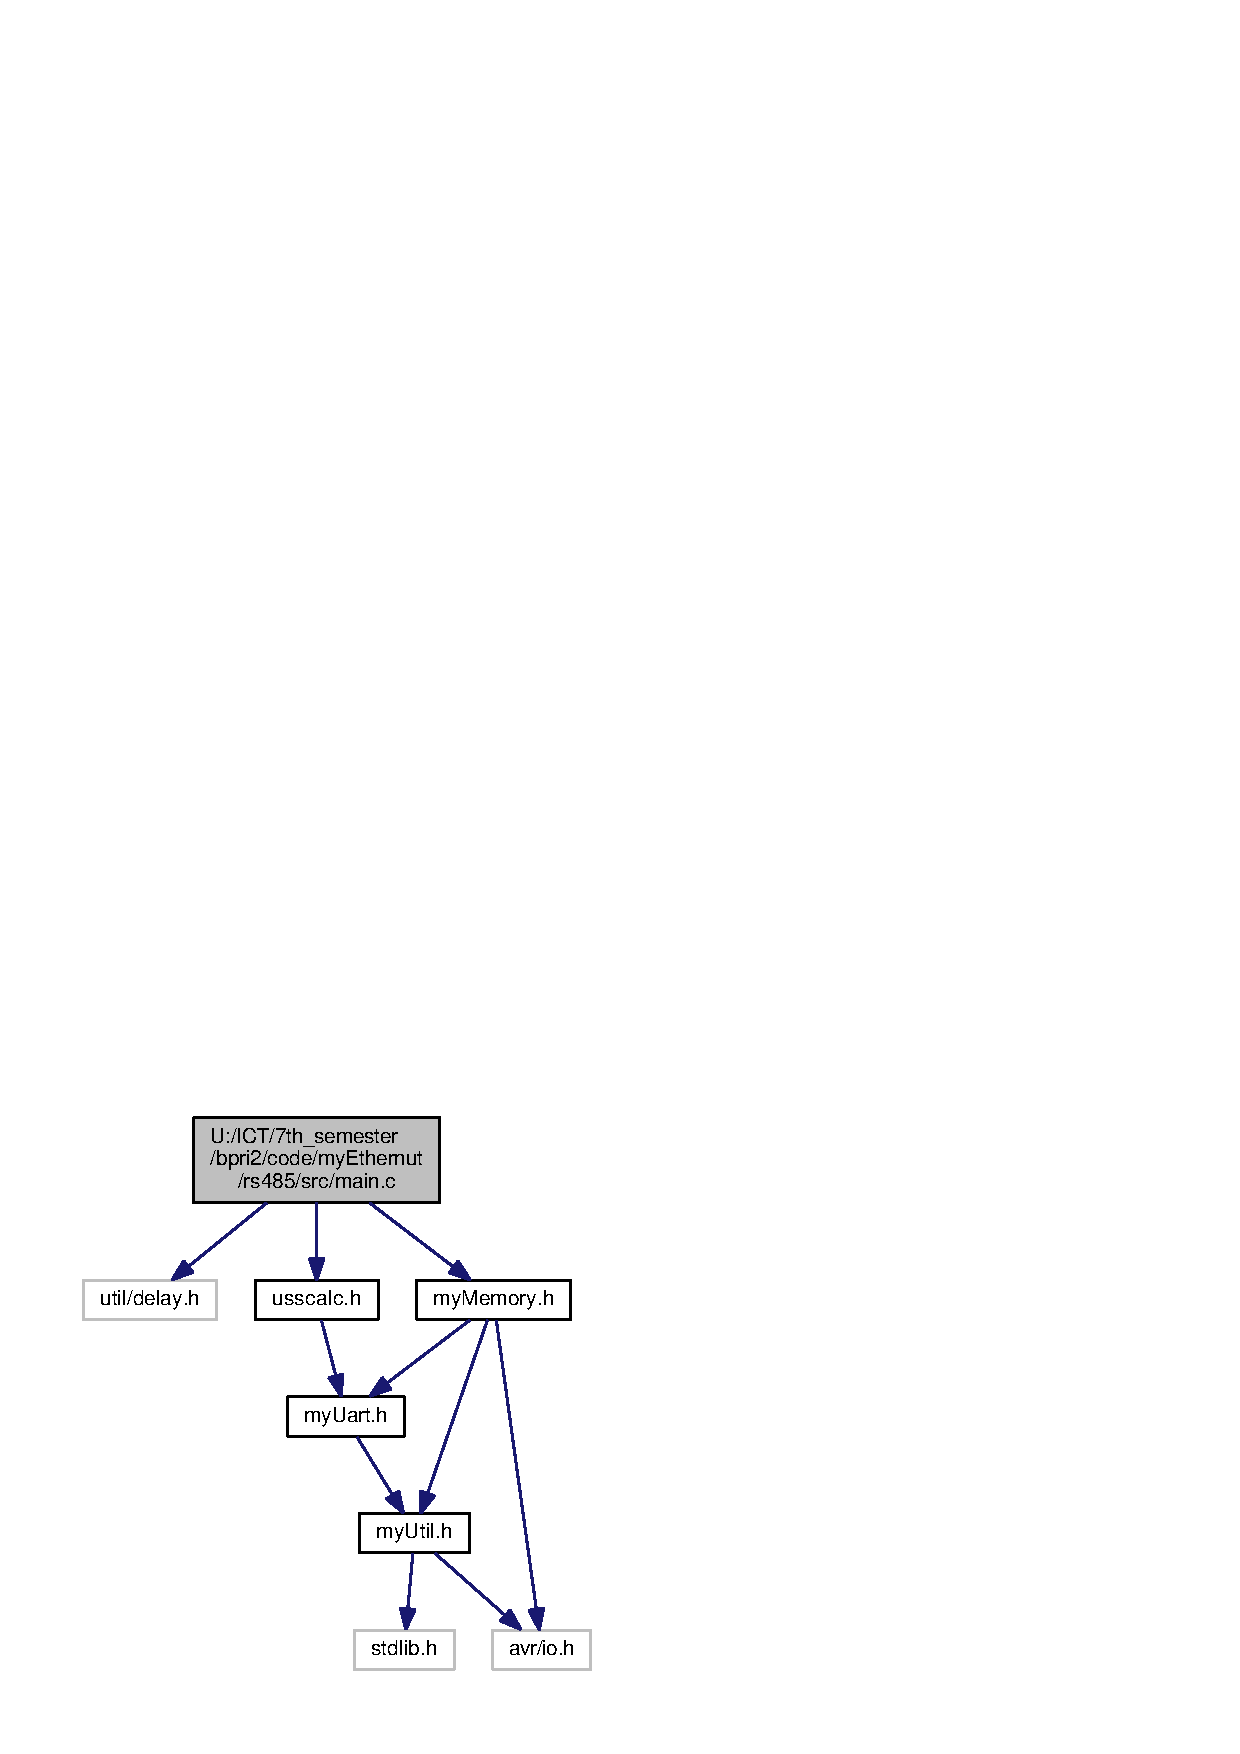
\includegraphics[width=350pt]{main_8c__incl}
\end{center}
\end{figure}
\doxysubsection*{Data Structures}
\begin{DoxyCompactItemize}
\item 
struct \mbox{\hyperlink{structparameter__struct}{parameter\+\_\+struct}}
\item 
struct \mbox{\hyperlink{struct_s_e_m_a_p_h_o_r_e___p_a_r_a_m_e_t_e_r_s}{S\+E\+M\+A\+P\+H\+O\+R\+E\+\_\+\+P\+A\+R\+A\+M\+E\+T\+E\+RS}}
\end{DoxyCompactItemize}
\doxysubsection*{Typedefs}
\begin{DoxyCompactItemize}
\item 
typedef struct \mbox{\hyperlink{structparameter__struct}{parameter\+\_\+struct}} \mbox{\hyperlink{main_8c_a4f866bc389d610b9af1569828c5cb796}{parameter\+\_\+struct\+\_\+t}}
\item 
typedef struct \mbox{\hyperlink{struct_s_e_m_a_p_h_o_r_e___p_a_r_a_m_e_t_e_r_s}{S\+E\+M\+A\+P\+H\+O\+R\+E\+\_\+\+P\+A\+R\+A\+M\+E\+T\+E\+RS}} \mbox{\hyperlink{main_8c_a8fa66a9bec224102af9be786a011d0ad}{x\+Semaphore\+Parameters\+\_\+t}}
\end{DoxyCompactItemize}
\doxysubsection*{Functions}
\begin{DoxyCompactItemize}
\item 
void \mbox{\hyperlink{main_8c_a0631242f9ef4df98c0aa08fc3477016b}{My\+L\+E\+Ds\+Toggling}} (uint8\+\_\+t tyle\+Razy)
\item 
void \mbox{\hyperlink{main_8c_a73549cfa09efe760d01971a22fd6b473}{My\+Error\+Handler}} (\mbox{\hyperlink{_generated_2_f_r_e_e_r_t_o_s_2task_8h_ae95f44d4cfeb4a599c6cc258d241cb6b}{Task\+Handle\+\_\+t}} x\+U\+A\+R\+T\+Handle)
\item 
void \mbox{\hyperlink{main_8c_a6a82a5f642a3795d49ee2a181494f472}{v\+Application\+Stack\+Overflow\+Hook}} (\mbox{\hyperlink{_model_2_a_p_p_s_2_f_r_e_e_r_t_o_s_2v4__1__2_2_templates_2_free_r_t_o_s_8h_af7cd8f53b62f0c497b442b504c30f2ec}{x\+Task\+Handle}} $\ast$px\+Task, signed char $\ast$pc\+Task\+Name)
\item 
void \mbox{\hyperlink{main_8c_a73f6aa45470ada02a5d6f3a522d8f13c}{v\+Application\+Malloc\+Failed\+Hook}} ()
\item 
void \mbox{\hyperlink{main_8c_afa643a0090e2cb938031a8ce2c46033c}{my\+Timer\+Callback}} (\mbox{\hyperlink{_model_2_a_p_p_s_2_f_r_e_e_r_t_o_s_2v4__1__2_2_templates_2_free_r_t_o_s_8h_a9fa57c444af781c3b6286f5cc9e4982d}{x\+Timer\+Handle}} px\+Timer)
\item 
int \mbox{\hyperlink{main_8c_a840291bc02cba5474a4cb46a9b9566fe}{main}} (void)
\end{DoxyCompactItemize}
\doxysubsection*{Variables}
\begin{DoxyCompactItemize}
\item 
\mbox{\hyperlink{_generated_2_f_r_e_e_r_t_o_s_2queue_8h_aaf19d499892a4ce1409326ece00f5264}{Queue\+Handle\+\_\+t}} \mbox{\hyperlink{main_8c_aa78b6121b7586233293fb6cba5e19206}{x\+Queue}} = N\+U\+LL
\item 
\mbox{\hyperlink{_model_2_a_p_p_s_2_f_r_e_e_r_t_o_s_2v4__1__2_2_templates_2_free_r_t_o_s_8h_a2b4ea2af4cc24db3cbd458722e96fa2f}{x\+Queue\+Handle}} \mbox{\hyperlink{main_8c_a1f474f190f107b23b637c1ec19339180}{Queue\+\_\+id}}
\item 
\mbox{\hyperlink{_model_2_a_p_p_s_2_f_r_e_e_r_t_o_s_2v4__1__2_2_templates_2_free_r_t_o_s_8h_a520d8cf032327581ece00e5bd8e03a75}{x\+Semaphore\+Handle}} \mbox{\hyperlink{main_8c_a518b536ed9bf3aae03f23de3ca80d69a}{notification\+\_\+semaphore}}
\item 
\mbox{\hyperlink{_model_2_a_p_p_s_2_f_r_e_e_r_t_o_s_2v4__1__2_2_templates_2_free_r_t_o_s_8h_a9fa57c444af781c3b6286f5cc9e4982d}{x\+Timer\+Handle}} \mbox{\hyperlink{main_8c_a02eac32cb5e7d9181d0197f353680c36}{Timer\+\_\+handle}}
\item 
\mbox{\hyperlink{_model_2_a_p_p_s_2_f_r_e_e_r_t_o_s_2v4__1__2_2_templates_2_free_r_t_o_s_8h_af7cd8f53b62f0c497b442b504c30f2ec}{x\+Task\+Handle}} \mbox{\hyperlink{main_8c_af9594ea483e4b18a36cc64c770a0b2a6}{U\+A\+R\+T\+Handle}} = N\+U\+LL
\item 
\mbox{\hyperlink{_model_2_a_p_p_s_2_f_r_e_e_r_t_o_s_2v4__1__2_2_templates_2_free_r_t_o_s_8h_af7cd8f53b62f0c497b442b504c30f2ec}{x\+Task\+Handle}} \mbox{\hyperlink{main_8c_aeb8570170354bebca19705854397cc75}{S\+P\+I\+Handle}} = N\+U\+LL
\item 
\mbox{\hyperlink{_model_2_a_p_p_s_2_f_r_e_e_r_t_o_s_2v4__1__2_2_templates_2_free_r_t_o_s_8h_af7cd8f53b62f0c497b442b504c30f2ec}{x\+Task\+Handle}} \mbox{\hyperlink{main_8c_a0322c8c10fc32d9da88dbb42525d11cd}{worker1\+\_\+id}}
\item 
\mbox{\hyperlink{_model_2_a_p_p_s_2_f_r_e_e_r_t_o_s_2v4__1__2_2_templates_2_free_r_t_o_s_8h_af7cd8f53b62f0c497b442b504c30f2ec}{x\+Task\+Handle}} \mbox{\hyperlink{main_8c_ae10999ad4b9b69ce410922e0a977066e}{worker2\+\_\+id}}
\end{DoxyCompactItemize}


\doxysubsection{Typedef Documentation}
\mbox{\Hypertarget{main_8c_a4f866bc389d610b9af1569828c5cb796}\label{main_8c_a4f866bc389d610b9af1569828c5cb796}} 
\index{main.c@{main.c}!parameter\_struct\_t@{parameter\_struct\_t}}
\index{parameter\_struct\_t@{parameter\_struct\_t}!main.c@{main.c}}
\doxysubsubsection{\texorpdfstring{parameter\_struct\_t}{parameter\_struct\_t}}
{\footnotesize\ttfamily typedef struct \mbox{\hyperlink{structparameter__struct}{parameter\+\_\+struct}} \mbox{\hyperlink{main_8c_a4f866bc389d610b9af1569828c5cb796}{parameter\+\_\+struct\+\_\+t}}}

\mbox{\Hypertarget{main_8c_a8fa66a9bec224102af9be786a011d0ad}\label{main_8c_a8fa66a9bec224102af9be786a011d0ad}} 
\index{main.c@{main.c}!xSemaphoreParameters\_t@{xSemaphoreParameters\_t}}
\index{xSemaphoreParameters\_t@{xSemaphoreParameters\_t}!main.c@{main.c}}
\doxysubsubsection{\texorpdfstring{xSemaphoreParameters\_t}{xSemaphoreParameters\_t}}
{\footnotesize\ttfamily typedef struct \mbox{\hyperlink{struct_s_e_m_a_p_h_o_r_e___p_a_r_a_m_e_t_e_r_s}{S\+E\+M\+A\+P\+H\+O\+R\+E\+\_\+\+P\+A\+R\+A\+M\+E\+T\+E\+RS}} \mbox{\hyperlink{main_8c_a8fa66a9bec224102af9be786a011d0ad}{x\+Semaphore\+Parameters\+\_\+t}}}



\doxysubsection{Function Documentation}
\mbox{\Hypertarget{main_8c_a840291bc02cba5474a4cb46a9b9566fe}\label{main_8c_a840291bc02cba5474a4cb46a9b9566fe}} 
\index{main.c@{main.c}!main@{main}}
\index{main@{main}!main.c@{main.c}}
\doxysubsubsection{\texorpdfstring{main()}{main()}}
{\footnotesize\ttfamily int main (\begin{DoxyParamCaption}\item[{void}]{ }\end{DoxyParamCaption})}



Definition at line 77 of file main.\+c.



References config\+M\+I\+N\+I\+M\+A\+L\+\_\+\+S\+T\+A\+C\+K\+\_\+\+S\+I\+ZE, D\+A\+V\+E\+\_\+\+Init(), D\+A\+V\+E\+\_\+\+S\+T\+A\+T\+U\+S\+\_\+\+S\+U\+C\+C\+E\+SS, Manager\+\_\+\+Task(), my\+Timer\+Callback(), pd\+T\+R\+UE, pv\+Port\+Malloc(), Queue\+\_\+id, Timer\+\_\+handle, tsk\+I\+D\+L\+E\+\_\+\+P\+R\+I\+O\+R\+I\+TY, v\+Task\+Start\+Scheduler(), worker1\+\_\+id, worker1\+\_\+task(), worker2\+\_\+id, worker2\+\_\+task(), X\+M\+C\+\_\+\+D\+E\+B\+UG, x\+Queue, x\+Timer\+Create(), and x\+Timer\+Start.

Here is the call graph for this function\+:
\nopagebreak
\begin{figure}[H]
\begin{center}
\leavevmode
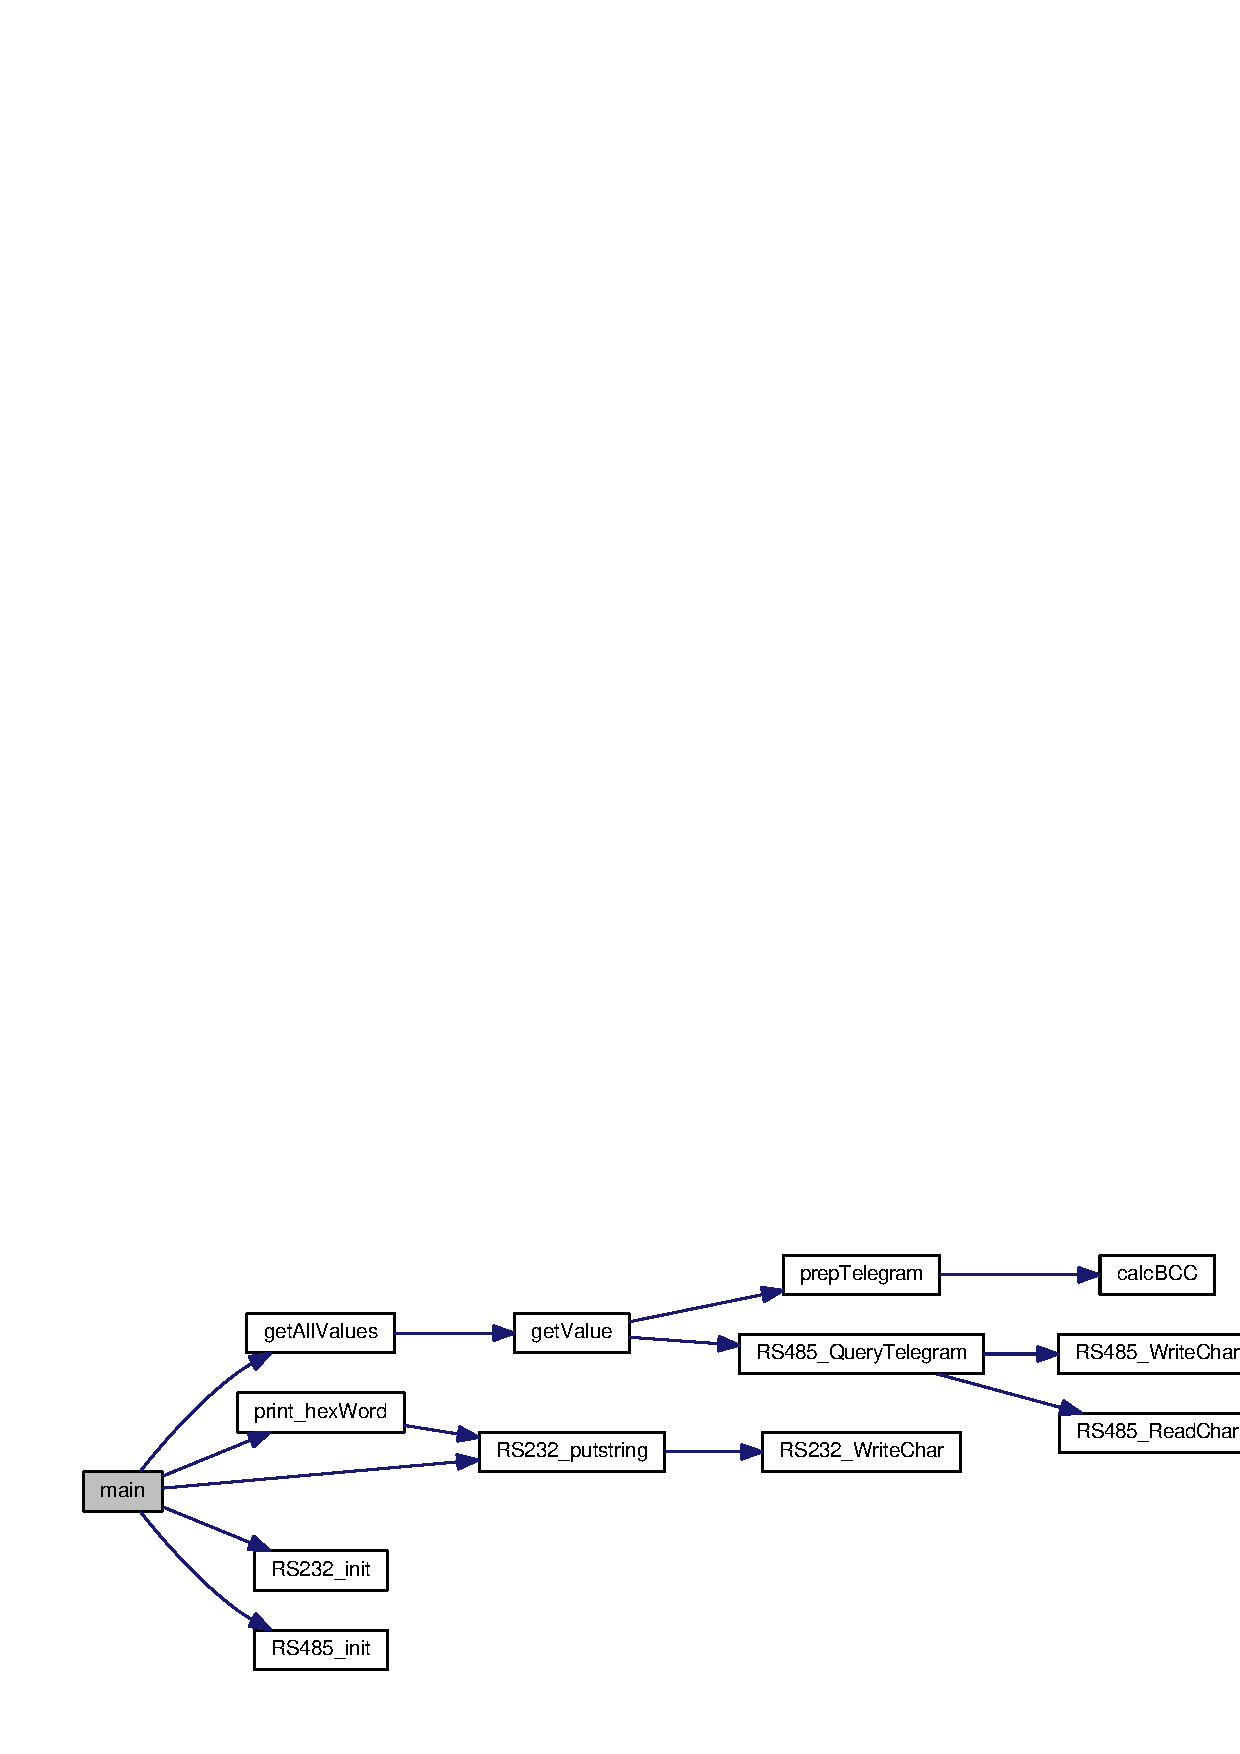
\includegraphics[width=350pt]{main_8c_a840291bc02cba5474a4cb46a9b9566fe_cgraph}
\end{center}
\end{figure}
\mbox{\Hypertarget{main_8c_a73549cfa09efe760d01971a22fd6b473}\label{main_8c_a73549cfa09efe760d01971a22fd6b473}} 
\index{main.c@{main.c}!MyErrorHandler@{MyErrorHandler}}
\index{MyErrorHandler@{MyErrorHandler}!main.c@{main.c}}
\doxysubsubsection{\texorpdfstring{MyErrorHandler()}{MyErrorHandler()}}
{\footnotesize\ttfamily void My\+Error\+Handler (\begin{DoxyParamCaption}\item[{\mbox{\hyperlink{_generated_2_f_r_e_e_r_t_o_s_2task_8h_ae95f44d4cfeb4a599c6cc258d241cb6b}{Task\+Handle\+\_\+t}}}]{x\+U\+A\+R\+T\+Handle }\end{DoxyParamCaption})}



Definition at line 42 of file main.\+c.



References My\+L\+E\+Ds\+Toggling(), pd\+M\+S\+\_\+\+T\+O\+\_\+\+T\+I\+C\+KS, v\+Task\+Delay(), and v\+Task\+Delete().

Here is the call graph for this function\+:
\nopagebreak
\begin{figure}[H]
\begin{center}
\leavevmode
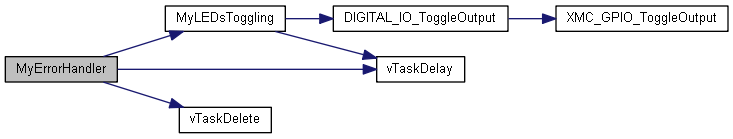
\includegraphics[width=350pt]{main_8c_a73549cfa09efe760d01971a22fd6b473_cgraph}
\end{center}
\end{figure}
\mbox{\Hypertarget{main_8c_a0631242f9ef4df98c0aa08fc3477016b}\label{main_8c_a0631242f9ef4df98c0aa08fc3477016b}} 
\index{main.c@{main.c}!MyLEDsToggling@{MyLEDsToggling}}
\index{MyLEDsToggling@{MyLEDsToggling}!main.c@{main.c}}
\doxysubsubsection{\texorpdfstring{MyLEDsToggling()}{MyLEDsToggling()}}
{\footnotesize\ttfamily void My\+L\+E\+Ds\+Toggling (\begin{DoxyParamCaption}\item[{uint8\+\_\+t}]{tyle\+Razy }\end{DoxyParamCaption})}



Definition at line 34 of file main.\+c.



References D\+I\+G\+I\+T\+A\+L\+\_\+\+I\+O\+\_\+\+Toggle\+Output(), L\+E\+D0, L\+E\+D1, and v\+Task\+Delay().



Referenced by My\+Error\+Handler(), v\+Application\+Malloc\+Failed\+Hook(), and v\+Application\+Stack\+Overflow\+Hook().

Here is the call graph for this function\+:
\nopagebreak
\begin{figure}[H]
\begin{center}
\leavevmode
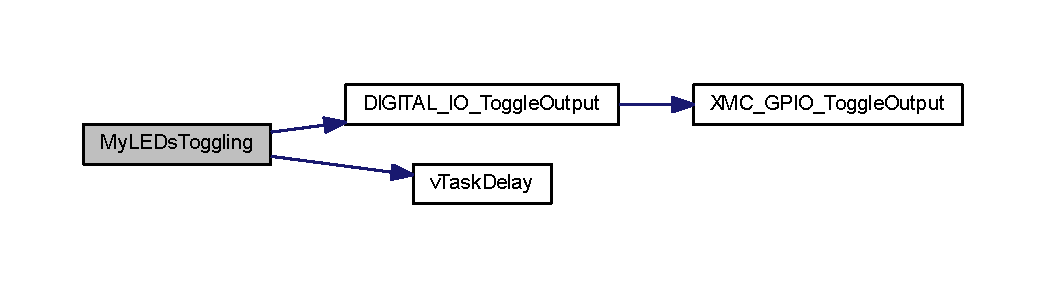
\includegraphics[width=350pt]{main_8c_a0631242f9ef4df98c0aa08fc3477016b_cgraph}
\end{center}
\end{figure}
\mbox{\Hypertarget{main_8c_afa643a0090e2cb938031a8ce2c46033c}\label{main_8c_afa643a0090e2cb938031a8ce2c46033c}} 
\index{main.c@{main.c}!myTimerCallback@{myTimerCallback}}
\index{myTimerCallback@{myTimerCallback}!main.c@{main.c}}
\doxysubsubsection{\texorpdfstring{myTimerCallback()}{myTimerCallback()}}
{\footnotesize\ttfamily void my\+Timer\+Callback (\begin{DoxyParamCaption}\item[{\mbox{\hyperlink{_model_2_a_p_p_s_2_f_r_e_e_r_t_o_s_2v4__1__2_2_templates_2_free_r_t_o_s_8h_a9fa57c444af781c3b6286f5cc9e4982d}{x\+Timer\+Handle}}}]{px\+Timer }\end{DoxyParamCaption})}



Definition at line 70 of file main.\+c.



References notification\+\_\+semaphore, and x\+Semaphore\+Give.



Referenced by main().

\mbox{\Hypertarget{main_8c_a73f6aa45470ada02a5d6f3a522d8f13c}\label{main_8c_a73f6aa45470ada02a5d6f3a522d8f13c}} 
\index{main.c@{main.c}!vApplicationMallocFailedHook@{vApplicationMallocFailedHook}}
\index{vApplicationMallocFailedHook@{vApplicationMallocFailedHook}!main.c@{main.c}}
\doxysubsubsection{\texorpdfstring{vApplicationMallocFailedHook()}{vApplicationMallocFailedHook()}}
{\footnotesize\ttfamily void v\+Application\+Malloc\+Failed\+Hook (\begin{DoxyParamCaption}{ }\end{DoxyParamCaption})}



Definition at line 63 of file main.\+c.



References My\+L\+E\+Ds\+Toggling(), pd\+M\+S\+\_\+\+T\+O\+\_\+\+T\+I\+C\+KS, and v\+Task\+Delay().



Referenced by pv\+Port\+Malloc().

Here is the call graph for this function\+:
\nopagebreak
\begin{figure}[H]
\begin{center}
\leavevmode
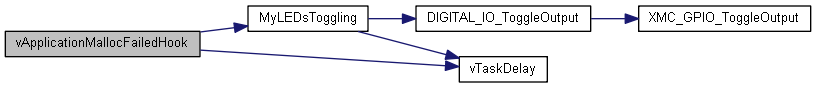
\includegraphics[width=350pt]{main_8c_a73f6aa45470ada02a5d6f3a522d8f13c_cgraph}
\end{center}
\end{figure}
\mbox{\Hypertarget{main_8c_a6a82a5f642a3795d49ee2a181494f472}\label{main_8c_a6a82a5f642a3795d49ee2a181494f472}} 
\index{main.c@{main.c}!vApplicationStackOverflowHook@{vApplicationStackOverflowHook}}
\index{vApplicationStackOverflowHook@{vApplicationStackOverflowHook}!main.c@{main.c}}
\doxysubsubsection{\texorpdfstring{vApplicationStackOverflowHook()}{vApplicationStackOverflowHook()}}
{\footnotesize\ttfamily void v\+Application\+Stack\+Overflow\+Hook (\begin{DoxyParamCaption}\item[{\mbox{\hyperlink{_model_2_a_p_p_s_2_f_r_e_e_r_t_o_s_2v4__1__2_2_templates_2_free_r_t_o_s_8h_af7cd8f53b62f0c497b442b504c30f2ec}{x\+Task\+Handle}} $\ast$}]{px\+Task,  }\item[{signed char $\ast$}]{pc\+Task\+Name }\end{DoxyParamCaption})}



Definition at line 53 of file main.\+c.



References My\+L\+E\+Ds\+Toggling(), pd\+M\+S\+\_\+\+T\+O\+\_\+\+T\+I\+C\+KS, and v\+Task\+Delay().

Here is the call graph for this function\+:
\nopagebreak
\begin{figure}[H]
\begin{center}
\leavevmode
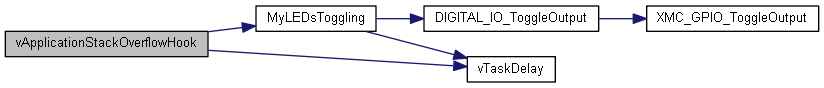
\includegraphics[width=350pt]{main_8c_a6a82a5f642a3795d49ee2a181494f472_cgraph}
\end{center}
\end{figure}


\doxysubsection{Variable Documentation}
\mbox{\Hypertarget{main_8c_a518b536ed9bf3aae03f23de3ca80d69a}\label{main_8c_a518b536ed9bf3aae03f23de3ca80d69a}} 
\index{main.c@{main.c}!notification\_semaphore@{notification\_semaphore}}
\index{notification\_semaphore@{notification\_semaphore}!main.c@{main.c}}
\doxysubsubsection{\texorpdfstring{notification\_semaphore}{notification\_semaphore}}
{\footnotesize\ttfamily \mbox{\hyperlink{_model_2_a_p_p_s_2_f_r_e_e_r_t_o_s_2v4__1__2_2_templates_2_free_r_t_o_s_8h_a520d8cf032327581ece00e5bd8e03a75}{x\+Semaphore\+Handle}} notification\+\_\+semaphore}



Definition at line 15 of file main.\+c.



Referenced by Manager\+\_\+\+Task(), and my\+Timer\+Callback().

\mbox{\Hypertarget{main_8c_a1f474f190f107b23b637c1ec19339180}\label{main_8c_a1f474f190f107b23b637c1ec19339180}} 
\index{main.c@{main.c}!Queue\_id@{Queue\_id}}
\index{Queue\_id@{Queue\_id}!main.c@{main.c}}
\doxysubsubsection{\texorpdfstring{Queue\_id}{Queue\_id}}
{\footnotesize\ttfamily \mbox{\hyperlink{_model_2_a_p_p_s_2_f_r_e_e_r_t_o_s_2v4__1__2_2_templates_2_free_r_t_o_s_8h_a2b4ea2af4cc24db3cbd458722e96fa2f}{x\+Queue\+Handle}} Queue\+\_\+id}



Definition at line 14 of file main.\+c.



Referenced by main(), Manager\+\_\+\+Task(), worker1\+\_\+task(), and worker2\+\_\+task().

\mbox{\Hypertarget{main_8c_aeb8570170354bebca19705854397cc75}\label{main_8c_aeb8570170354bebca19705854397cc75}} 
\index{main.c@{main.c}!SPIHandle@{SPIHandle}}
\index{SPIHandle@{SPIHandle}!main.c@{main.c}}
\doxysubsubsection{\texorpdfstring{SPIHandle}{SPIHandle}}
{\footnotesize\ttfamily \mbox{\hyperlink{_model_2_a_p_p_s_2_f_r_e_e_r_t_o_s_2v4__1__2_2_templates_2_free_r_t_o_s_8h_af7cd8f53b62f0c497b442b504c30f2ec}{x\+Task\+Handle}} S\+P\+I\+Handle = N\+U\+LL}



Definition at line 18 of file main.\+c.

\mbox{\Hypertarget{main_8c_a02eac32cb5e7d9181d0197f353680c36}\label{main_8c_a02eac32cb5e7d9181d0197f353680c36}} 
\index{main.c@{main.c}!Timer\_handle@{Timer\_handle}}
\index{Timer\_handle@{Timer\_handle}!main.c@{main.c}}
\doxysubsubsection{\texorpdfstring{Timer\_handle}{Timer\_handle}}
{\footnotesize\ttfamily \mbox{\hyperlink{_model_2_a_p_p_s_2_f_r_e_e_r_t_o_s_2v4__1__2_2_templates_2_free_r_t_o_s_8h_a9fa57c444af781c3b6286f5cc9e4982d}{x\+Timer\+Handle}} Timer\+\_\+handle}



Definition at line 16 of file main.\+c.



Referenced by main().

\mbox{\Hypertarget{main_8c_af9594ea483e4b18a36cc64c770a0b2a6}\label{main_8c_af9594ea483e4b18a36cc64c770a0b2a6}} 
\index{main.c@{main.c}!UARTHandle@{UARTHandle}}
\index{UARTHandle@{UARTHandle}!main.c@{main.c}}
\doxysubsubsection{\texorpdfstring{UARTHandle}{UARTHandle}}
{\footnotesize\ttfamily \mbox{\hyperlink{_model_2_a_p_p_s_2_f_r_e_e_r_t_o_s_2v4__1__2_2_templates_2_free_r_t_o_s_8h_af7cd8f53b62f0c497b442b504c30f2ec}{x\+Task\+Handle}} U\+A\+R\+T\+Handle = N\+U\+LL}



Definition at line 17 of file main.\+c.

\mbox{\Hypertarget{main_8c_a0322c8c10fc32d9da88dbb42525d11cd}\label{main_8c_a0322c8c10fc32d9da88dbb42525d11cd}} 
\index{main.c@{main.c}!worker1\_id@{worker1\_id}}
\index{worker1\_id@{worker1\_id}!main.c@{main.c}}
\doxysubsubsection{\texorpdfstring{worker1\_id}{worker1\_id}}
{\footnotesize\ttfamily \mbox{\hyperlink{_model_2_a_p_p_s_2_f_r_e_e_r_t_o_s_2v4__1__2_2_templates_2_free_r_t_o_s_8h_af7cd8f53b62f0c497b442b504c30f2ec}{x\+Task\+Handle}} worker1\+\_\+id}



Definition at line 19 of file main.\+c.



Referenced by main(), Manager\+\_\+\+Task(), and worker1\+\_\+task().

\mbox{\Hypertarget{main_8c_ae10999ad4b9b69ce410922e0a977066e}\label{main_8c_ae10999ad4b9b69ce410922e0a977066e}} 
\index{main.c@{main.c}!worker2\_id@{worker2\_id}}
\index{worker2\_id@{worker2\_id}!main.c@{main.c}}
\doxysubsubsection{\texorpdfstring{worker2\_id}{worker2\_id}}
{\footnotesize\ttfamily \mbox{\hyperlink{_model_2_a_p_p_s_2_f_r_e_e_r_t_o_s_2v4__1__2_2_templates_2_free_r_t_o_s_8h_af7cd8f53b62f0c497b442b504c30f2ec}{x\+Task\+Handle}} worker2\+\_\+id}



Definition at line 20 of file main.\+c.



Referenced by main(), Manager\+\_\+\+Task(), and worker2\+\_\+task().

\mbox{\Hypertarget{main_8c_aa78b6121b7586233293fb6cba5e19206}\label{main_8c_aa78b6121b7586233293fb6cba5e19206}} 
\index{main.c@{main.c}!xQueue@{xQueue}}
\index{xQueue@{xQueue}!main.c@{main.c}}
\doxysubsubsection{\texorpdfstring{xQueue}{xQueue}}
{\footnotesize\ttfamily \mbox{\hyperlink{_generated_2_f_r_e_e_r_t_o_s_2queue_8h_aaf19d499892a4ce1409326ece00f5264}{Queue\+Handle\+\_\+t}} x\+Queue = N\+U\+LL}



Definition at line 13 of file main.\+c.



Referenced by main(), pc\+Queue\+Get\+Name(), S\+P\+I\+\_\+\+Slave\+\_\+\+Task(), U\+A\+R\+T\+\_\+\+Task(), uc\+Queue\+Get\+Queue\+Type(), ux\+Queue\+Get\+Queue\+Number(), ux\+Queue\+Messages\+Waiting(), ux\+Queue\+Messages\+Waiting\+From\+I\+S\+R(), ux\+Queue\+Spaces\+Available(), v\+Queue\+Add\+To\+Registry(), v\+Queue\+Delete(), v\+Queue\+Set\+Queue\+Number(), v\+Queue\+Unregister\+Queue(), v\+Queue\+Wait\+For\+Message\+Restricted(), x\+Queue\+Generic\+Reset(), x\+Queue\+Generic\+Send(), x\+Queue\+Generic\+Send\+From\+I\+S\+R(), x\+Queue\+Give\+From\+I\+S\+R(), x\+Queue\+Is\+Queue\+Empty\+From\+I\+S\+R(), x\+Queue\+Is\+Queue\+Full\+From\+I\+S\+R(), x\+Queue\+Peek(), x\+Queue\+Peek\+From\+I\+S\+R(), x\+Queue\+Receive(), x\+Queue\+Receive\+From\+I\+S\+R(), and x\+Queue\+Semaphore\+Take().


\section{U\+:/\+I\+C\+T/7th\+\_\+semester/bpri2/code/my\+Ethernut/rs485/src/my\+Memory.c File Reference}
\label{my_memory_8c}\index{U\+:/\+I\+C\+T/7th\+\_\+semester/bpri2/code/my\+Ethernut/rs485/src/my\+Memory.\+c@{U\+:/\+I\+C\+T/7th\+\_\+semester/bpri2/code/my\+Ethernut/rs485/src/my\+Memory.\+c}}
{\ttfamily \#include \char`\"{}my\+Memory.\+h\char`\"{}}\\*
Include dependency graph for my\+Memory.\+c\+:\nopagebreak
\begin{figure}[H]
\begin{center}
\leavevmode
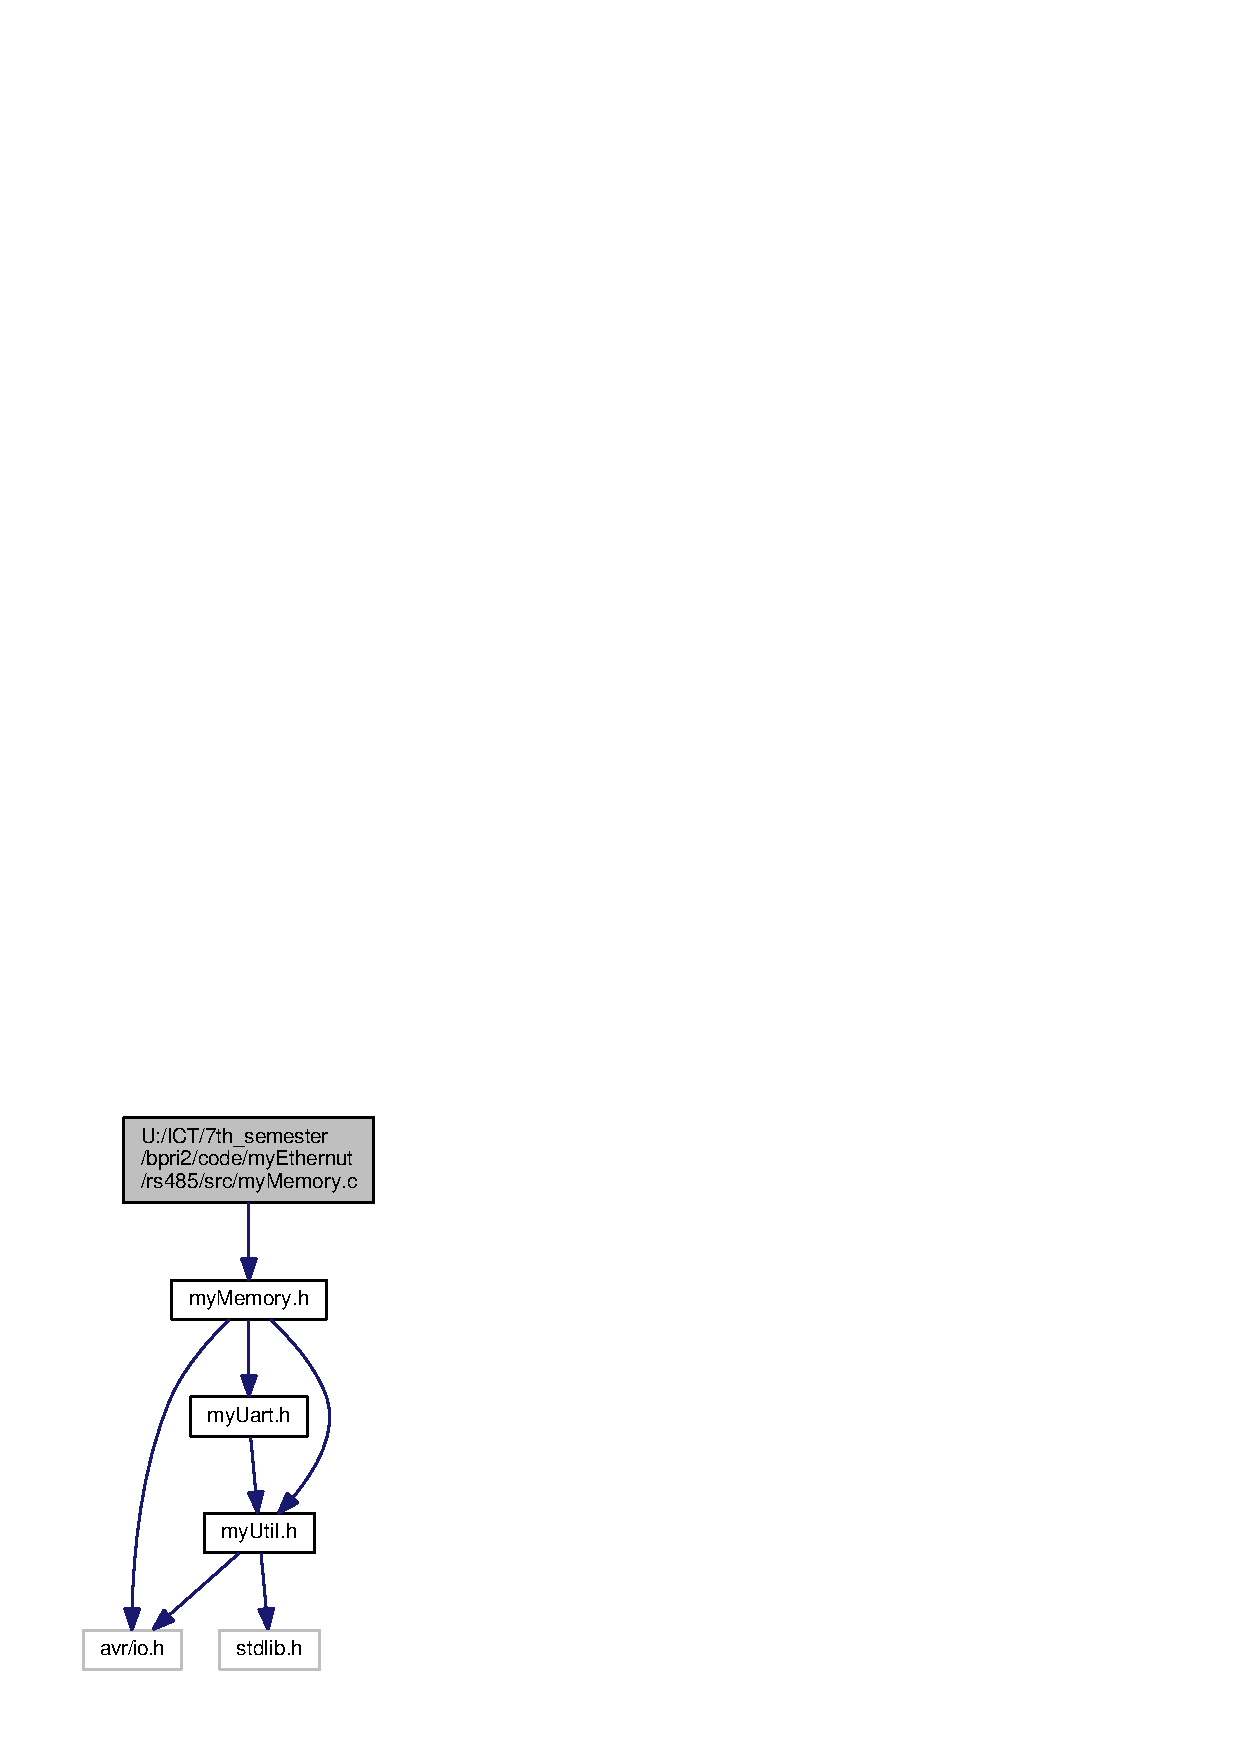
\includegraphics[width=184pt]{my_memory_8c__incl}
\end{center}
\end{figure}
\subsection*{Functions}
\begin{DoxyCompactItemize}
\item 
void {\bf test\+Memory} ()
\item 
void {\bf read\+R\+T\+L\+Memory} ()
\item 
void {\bf X\+M\+E\+M\+\_\+init} (void)
\end{DoxyCompactItemize}


\subsection{Function Documentation}
\index{my\+Memory.\+c@{my\+Memory.\+c}!read\+R\+T\+L\+Memory@{read\+R\+T\+L\+Memory}}
\index{read\+R\+T\+L\+Memory@{read\+R\+T\+L\+Memory}!my\+Memory.\+c@{my\+Memory.\+c}}
\subsubsection[{read\+R\+T\+L\+Memory()}]{\setlength{\rightskip}{0pt plus 5cm}void read\+R\+T\+L\+Memory (
\begin{DoxyParamCaption}
{}
\end{DoxyParamCaption}
)}\label{my_memory_8c_aee405b5e49f9825c385778bbbdb4f36b}


Definition at line 57 of file my\+Memory.\+c.



References print\+\_\+hex\+Address(), print\+\_\+hex\+Word(), and R\+S232\+\_\+putstring().



Here is the call graph for this function\+:\nopagebreak
\begin{figure}[H]
\begin{center}
\leavevmode
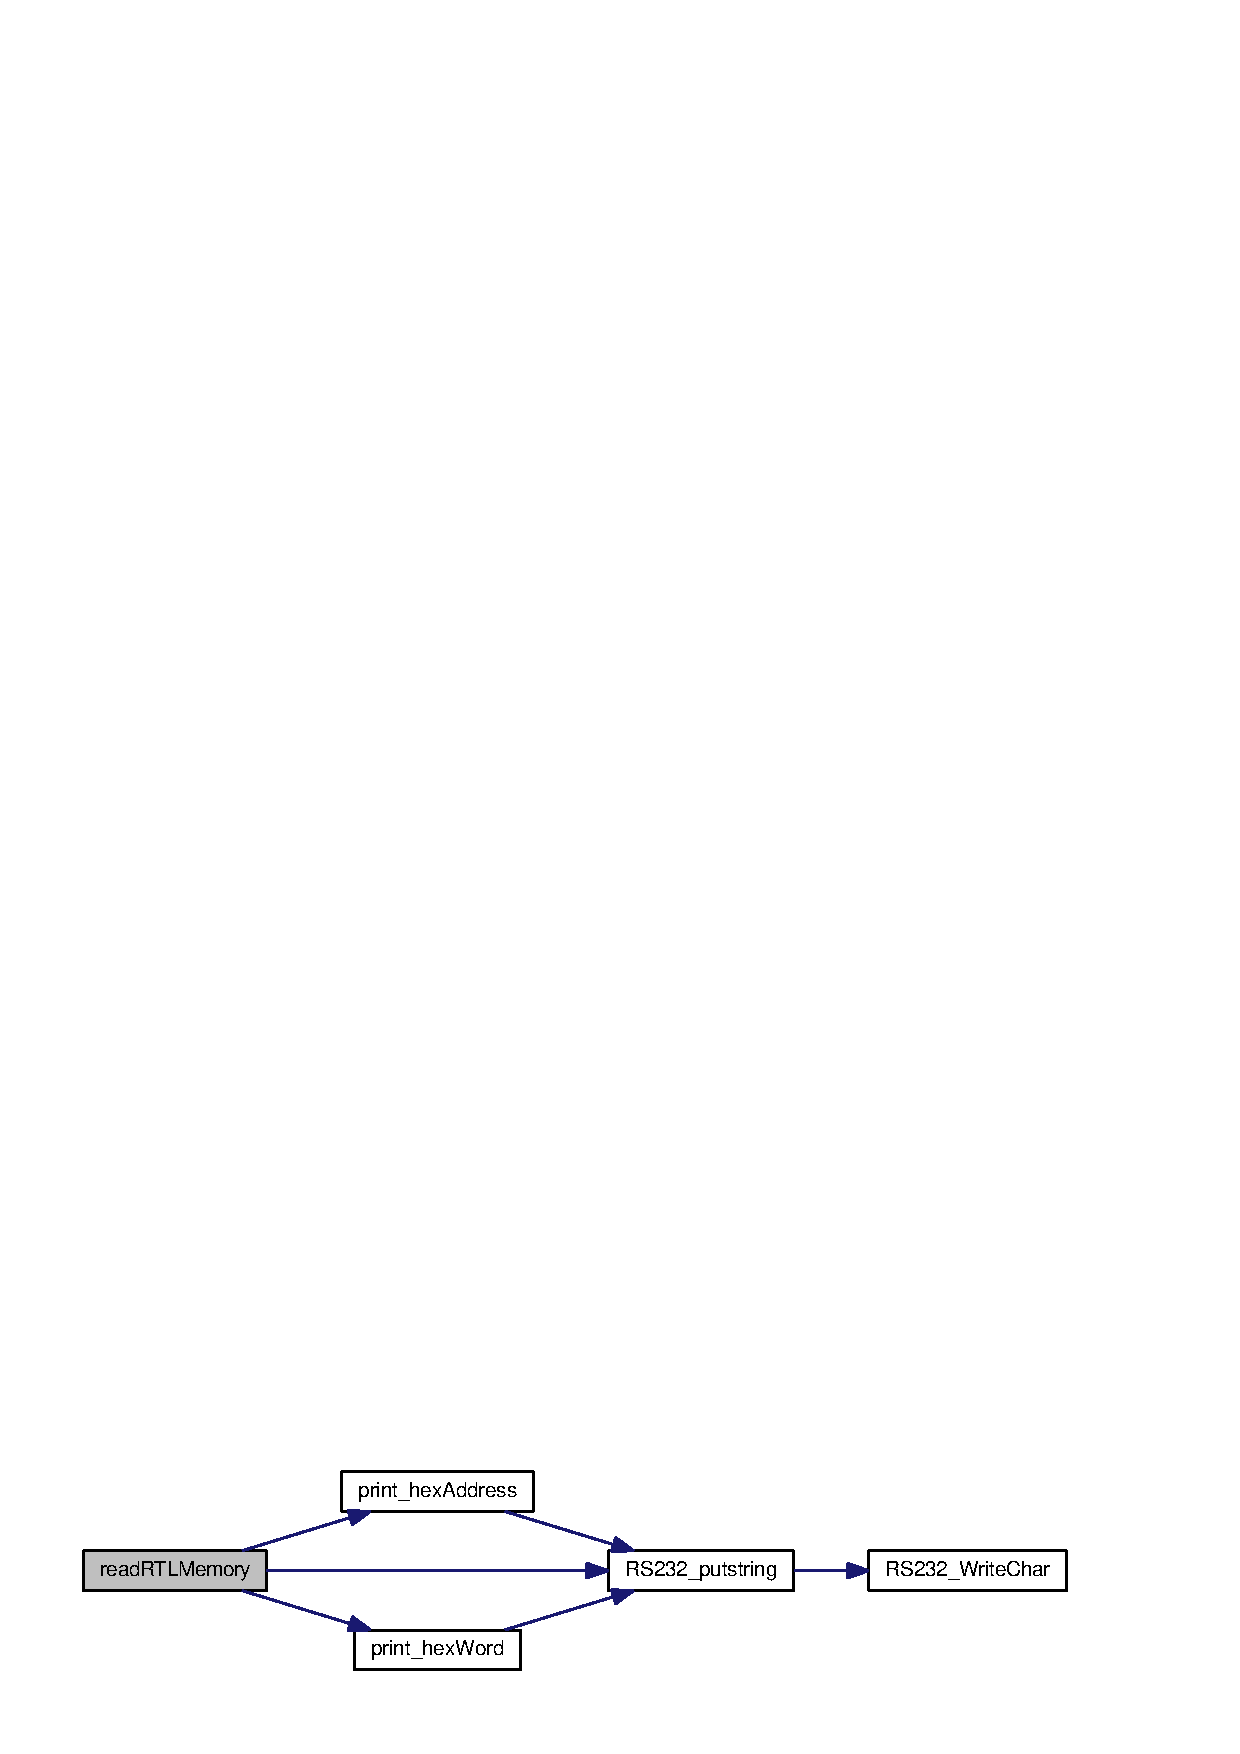
\includegraphics[width=350pt]{my_memory_8c_aee405b5e49f9825c385778bbbdb4f36b_cgraph}
\end{center}
\end{figure}


\index{my\+Memory.\+c@{my\+Memory.\+c}!test\+Memory@{test\+Memory}}
\index{test\+Memory@{test\+Memory}!my\+Memory.\+c@{my\+Memory.\+c}}
\subsubsection[{test\+Memory()}]{\setlength{\rightskip}{0pt plus 5cm}void test\+Memory (
\begin{DoxyParamCaption}
{}
\end{DoxyParamCaption}
)}\label{my_memory_8c_ae811c849e7999d4868458fffe1f87f8e}


Definition at line 4 of file my\+Memory.\+c.



References print\+\_\+hex\+Address(), print\+\_\+hex\+Word(), and R\+S232\+\_\+putstring().



Here is the call graph for this function\+:\nopagebreak
\begin{figure}[H]
\begin{center}
\leavevmode
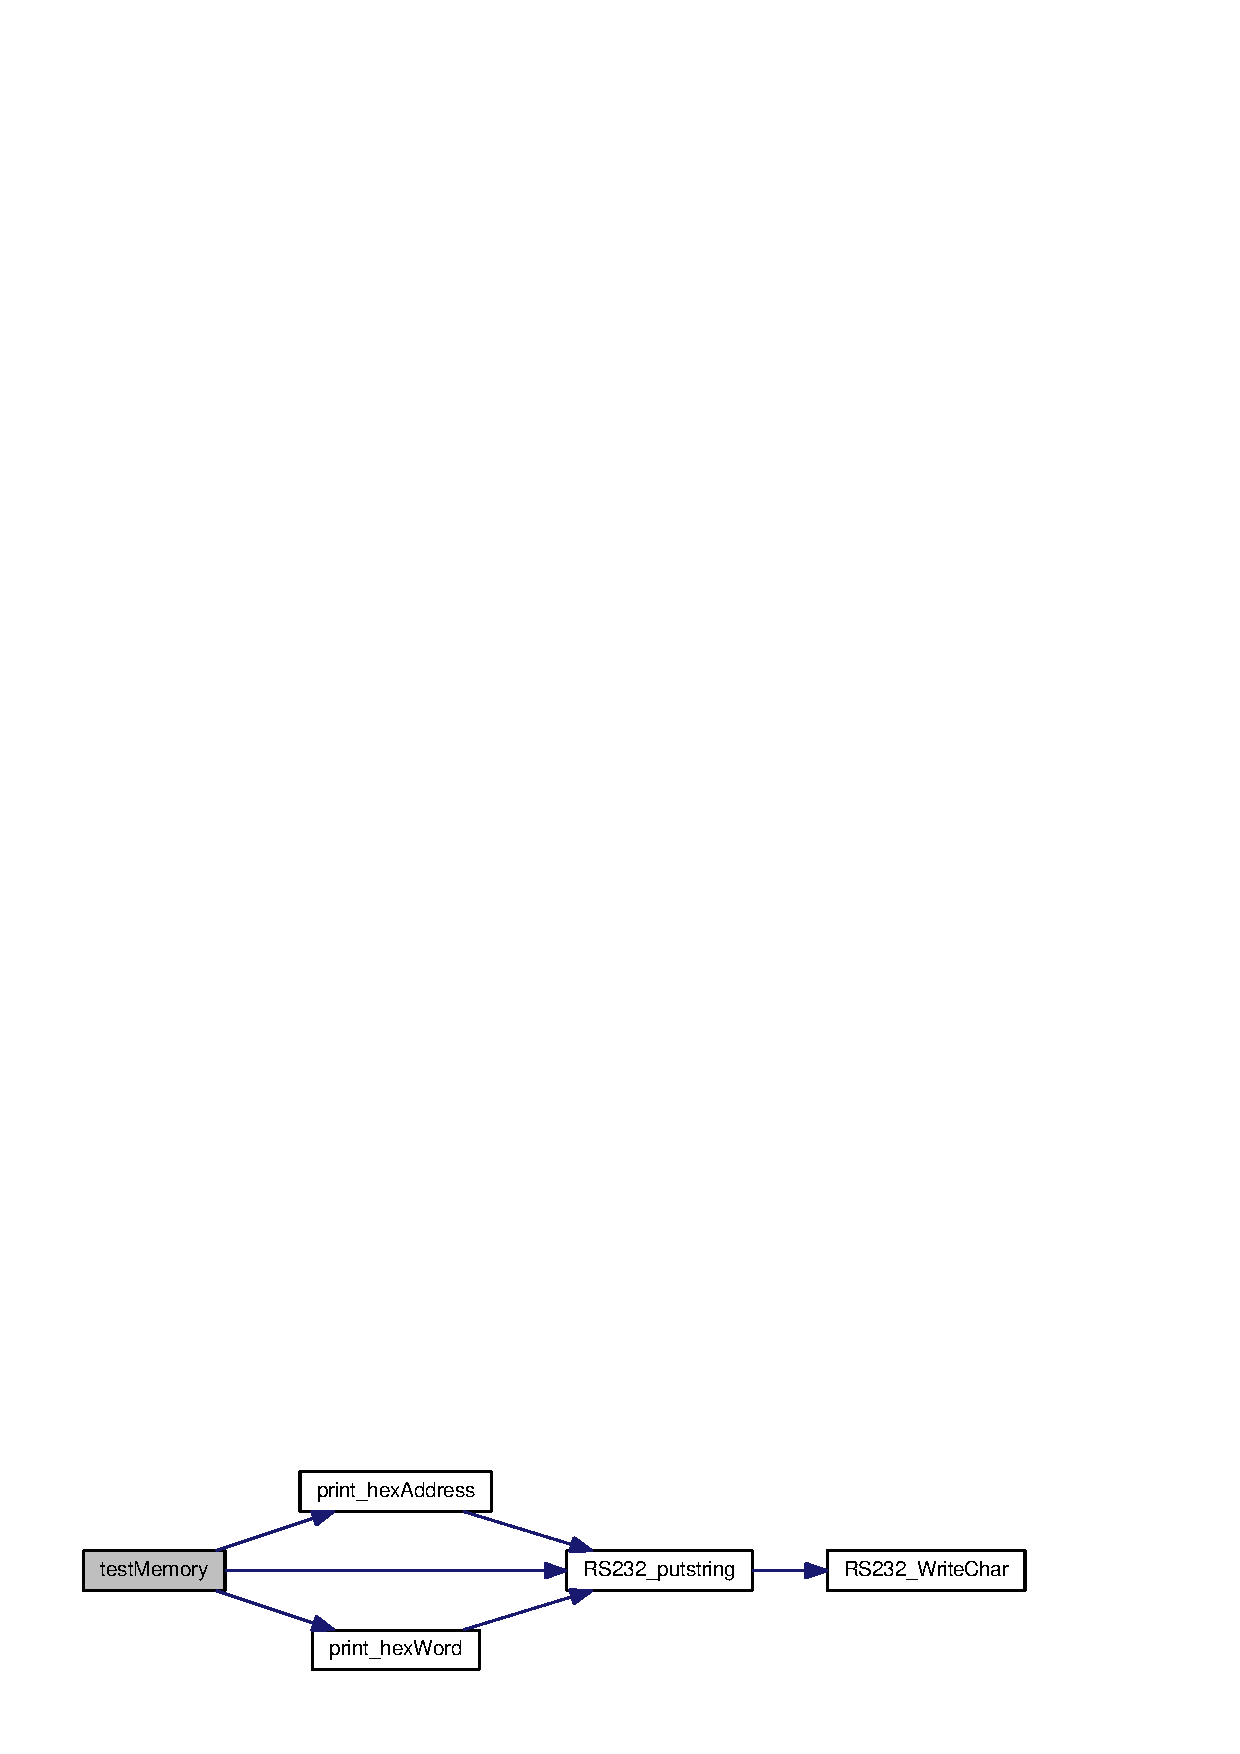
\includegraphics[width=350pt]{my_memory_8c_ae811c849e7999d4868458fffe1f87f8e_cgraph}
\end{center}
\end{figure}


\index{my\+Memory.\+c@{my\+Memory.\+c}!X\+M\+E\+M\+\_\+init@{X\+M\+E\+M\+\_\+init}}
\index{X\+M\+E\+M\+\_\+init@{X\+M\+E\+M\+\_\+init}!my\+Memory.\+c@{my\+Memory.\+c}}
\subsubsection[{X\+M\+E\+M\+\_\+init(void)}]{\setlength{\rightskip}{0pt plus 5cm}void X\+M\+E\+M\+\_\+init (
\begin{DoxyParamCaption}
\item[{void}]{}
\end{DoxyParamCaption}
)}\label{my_memory_8c_aa40171b2238355469afb6141d6f9d612}


Definition at line 113 of file my\+Memory.\+c.


\section{U\+:/\+I\+C\+T/7th\+\_\+semester/bpri2/code/my\+Ethernut/rs485/src/my\+Memory.h File Reference}
\label{my_memory_8h}\index{U\+:/\+I\+C\+T/7th\+\_\+semester/bpri2/code/my\+Ethernut/rs485/src/my\+Memory.\+h@{U\+:/\+I\+C\+T/7th\+\_\+semester/bpri2/code/my\+Ethernut/rs485/src/my\+Memory.\+h}}
{\ttfamily \#include $<$avr/io.\+h$>$}\\*
{\ttfamily \#include \char`\"{}my\+Uart.\+h\char`\"{}}\\*
{\ttfamily \#include \char`\"{}my\+Util.\+h\char`\"{}}\\*
Include dependency graph for my\+Memory.\+h\+:\nopagebreak
\begin{figure}[H]
\begin{center}
\leavevmode
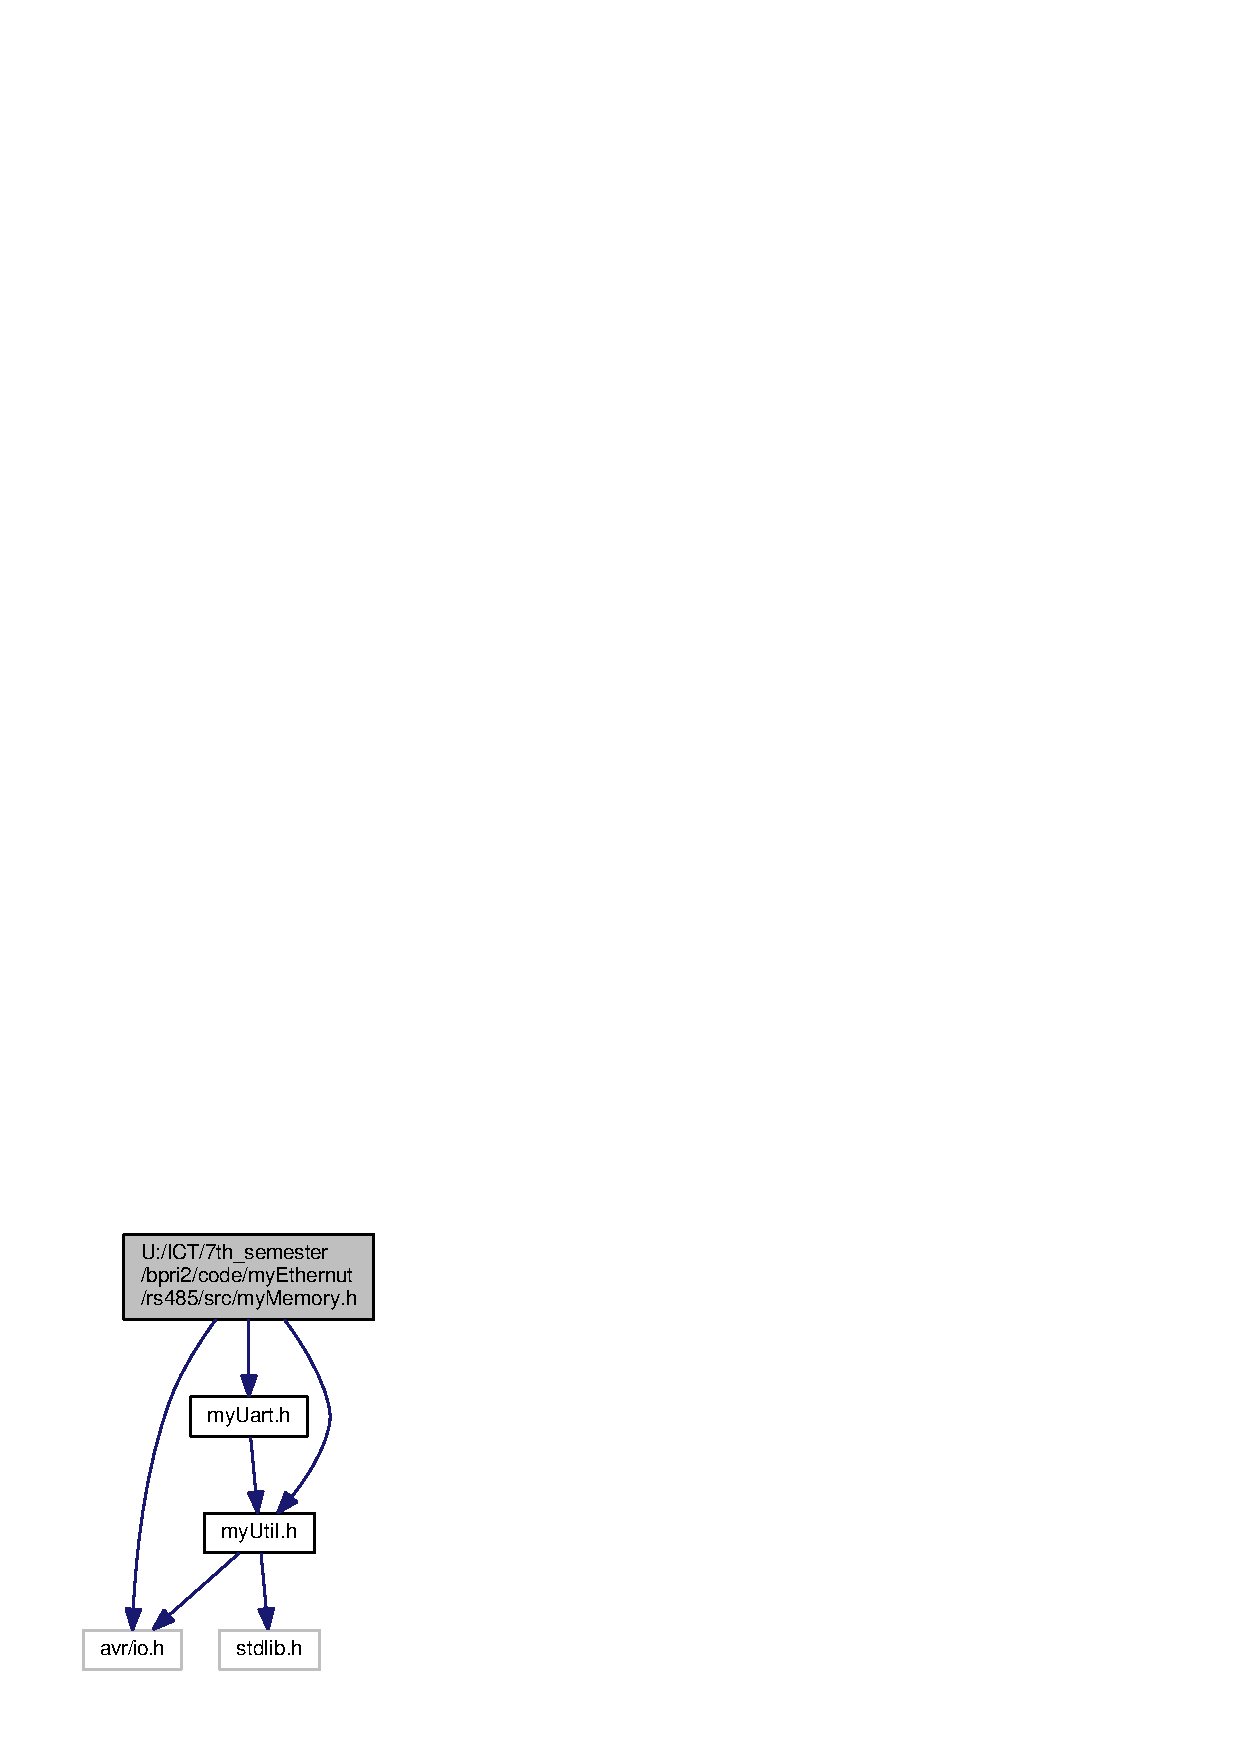
\includegraphics[width=184pt]{my_memory_8h__incl}
\end{center}
\end{figure}
This graph shows which files directly or indirectly include this file\+:\nopagebreak
\begin{figure}[H]
\begin{center}
\leavevmode
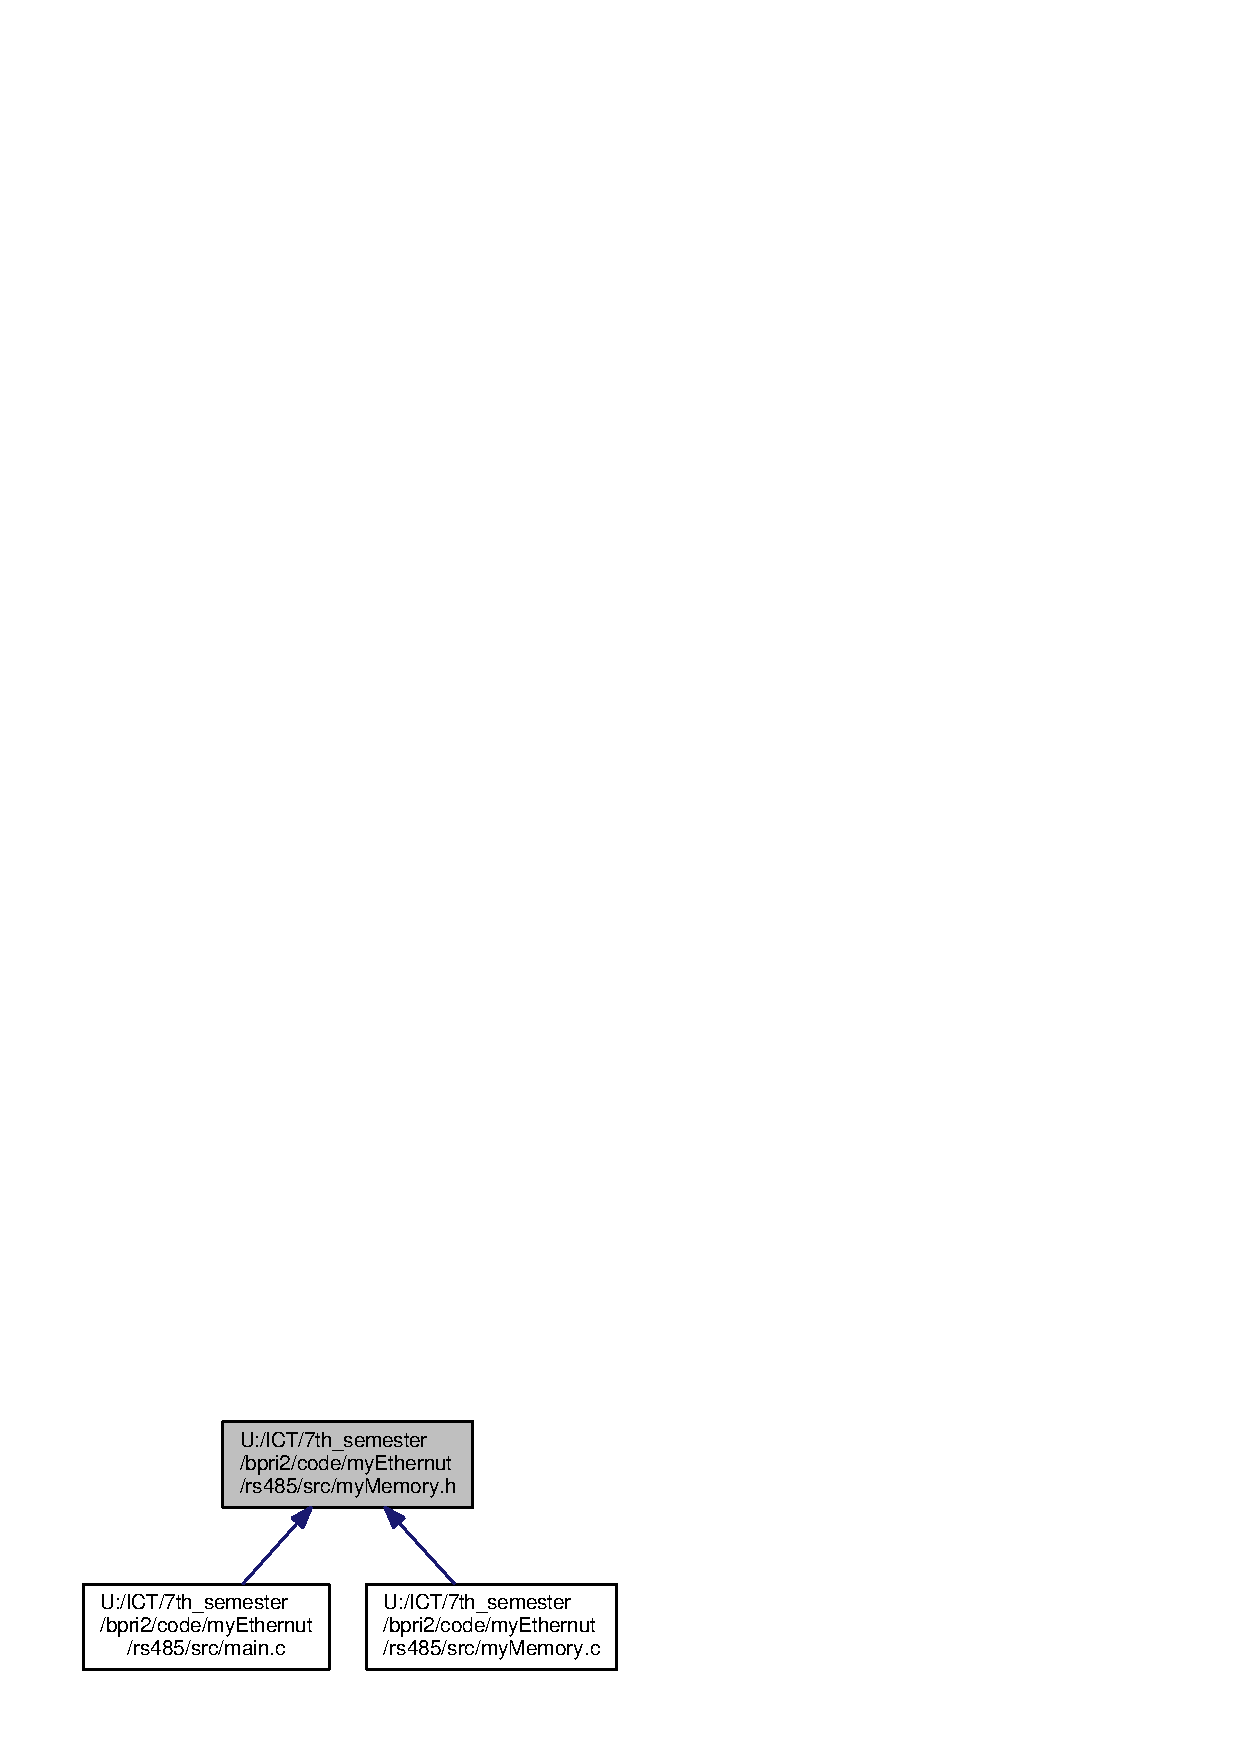
\includegraphics[width=300pt]{my_memory_8h__dep__incl}
\end{center}
\end{figure}
\subsection*{Functions}
\begin{DoxyCompactItemize}
\item 
void {\bf test\+Memory} ()
\item 
void {\bf read\+R\+T\+L\+Memory} ()
\item 
void {\bf X\+M\+E\+M\+\_\+init} (void)
\end{DoxyCompactItemize}


\subsection{Function Documentation}
\index{my\+Memory.\+h@{my\+Memory.\+h}!read\+R\+T\+L\+Memory@{read\+R\+T\+L\+Memory}}
\index{read\+R\+T\+L\+Memory@{read\+R\+T\+L\+Memory}!my\+Memory.\+h@{my\+Memory.\+h}}
\subsubsection[{read\+R\+T\+L\+Memory()}]{\setlength{\rightskip}{0pt plus 5cm}void read\+R\+T\+L\+Memory (
\begin{DoxyParamCaption}
{}
\end{DoxyParamCaption}
)}\label{my_memory_8h_aee405b5e49f9825c385778bbbdb4f36b}


Definition at line 57 of file my\+Memory.\+c.



References print\+\_\+hex\+Address(), print\+\_\+hex\+Word(), and R\+S232\+\_\+putstring().



Here is the call graph for this function\+:\nopagebreak
\begin{figure}[H]
\begin{center}
\leavevmode
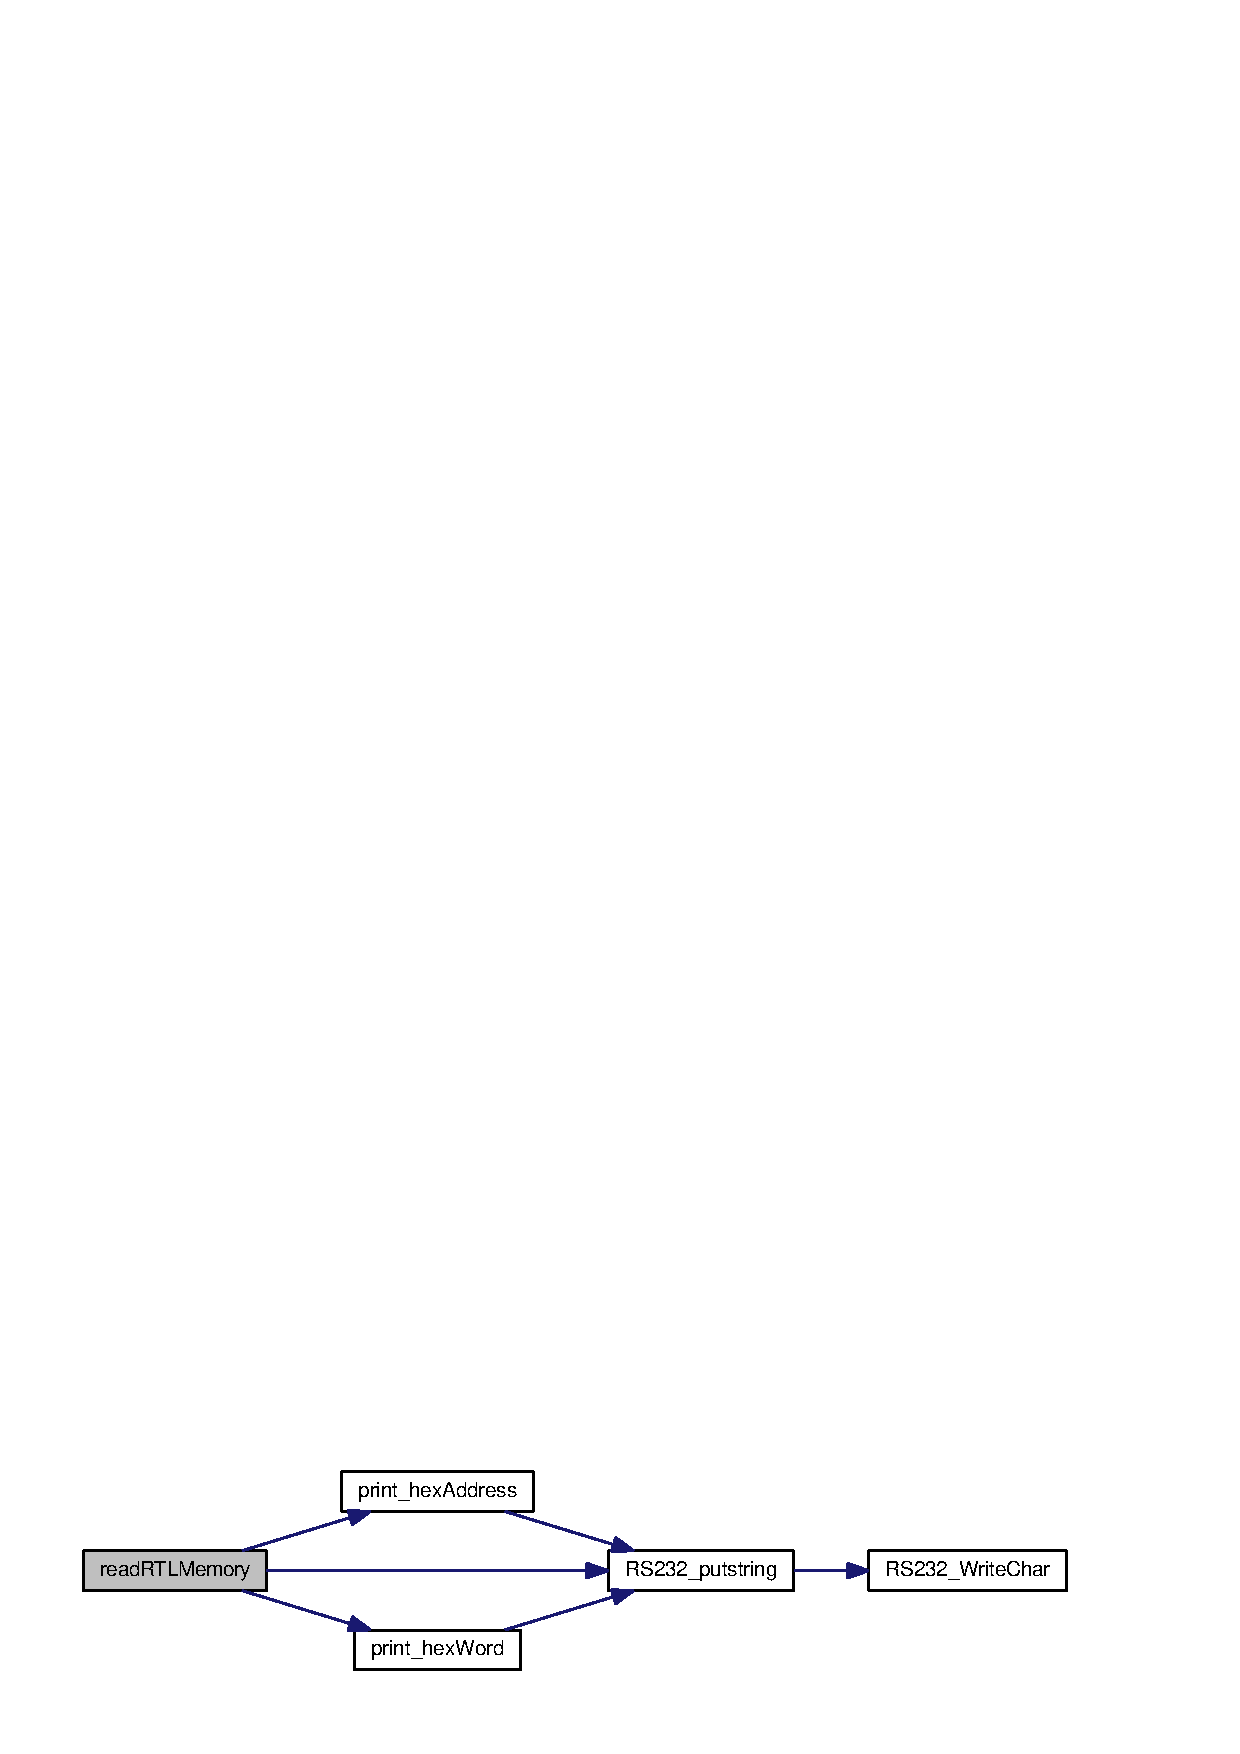
\includegraphics[width=350pt]{my_memory_8h_aee405b5e49f9825c385778bbbdb4f36b_cgraph}
\end{center}
\end{figure}


\index{my\+Memory.\+h@{my\+Memory.\+h}!test\+Memory@{test\+Memory}}
\index{test\+Memory@{test\+Memory}!my\+Memory.\+h@{my\+Memory.\+h}}
\subsubsection[{test\+Memory()}]{\setlength{\rightskip}{0pt plus 5cm}void test\+Memory (
\begin{DoxyParamCaption}
{}
\end{DoxyParamCaption}
)}\label{my_memory_8h_ae811c849e7999d4868458fffe1f87f8e}


Definition at line 4 of file my\+Memory.\+c.



References print\+\_\+hex\+Address(), print\+\_\+hex\+Word(), and R\+S232\+\_\+putstring().



Here is the call graph for this function\+:\nopagebreak
\begin{figure}[H]
\begin{center}
\leavevmode
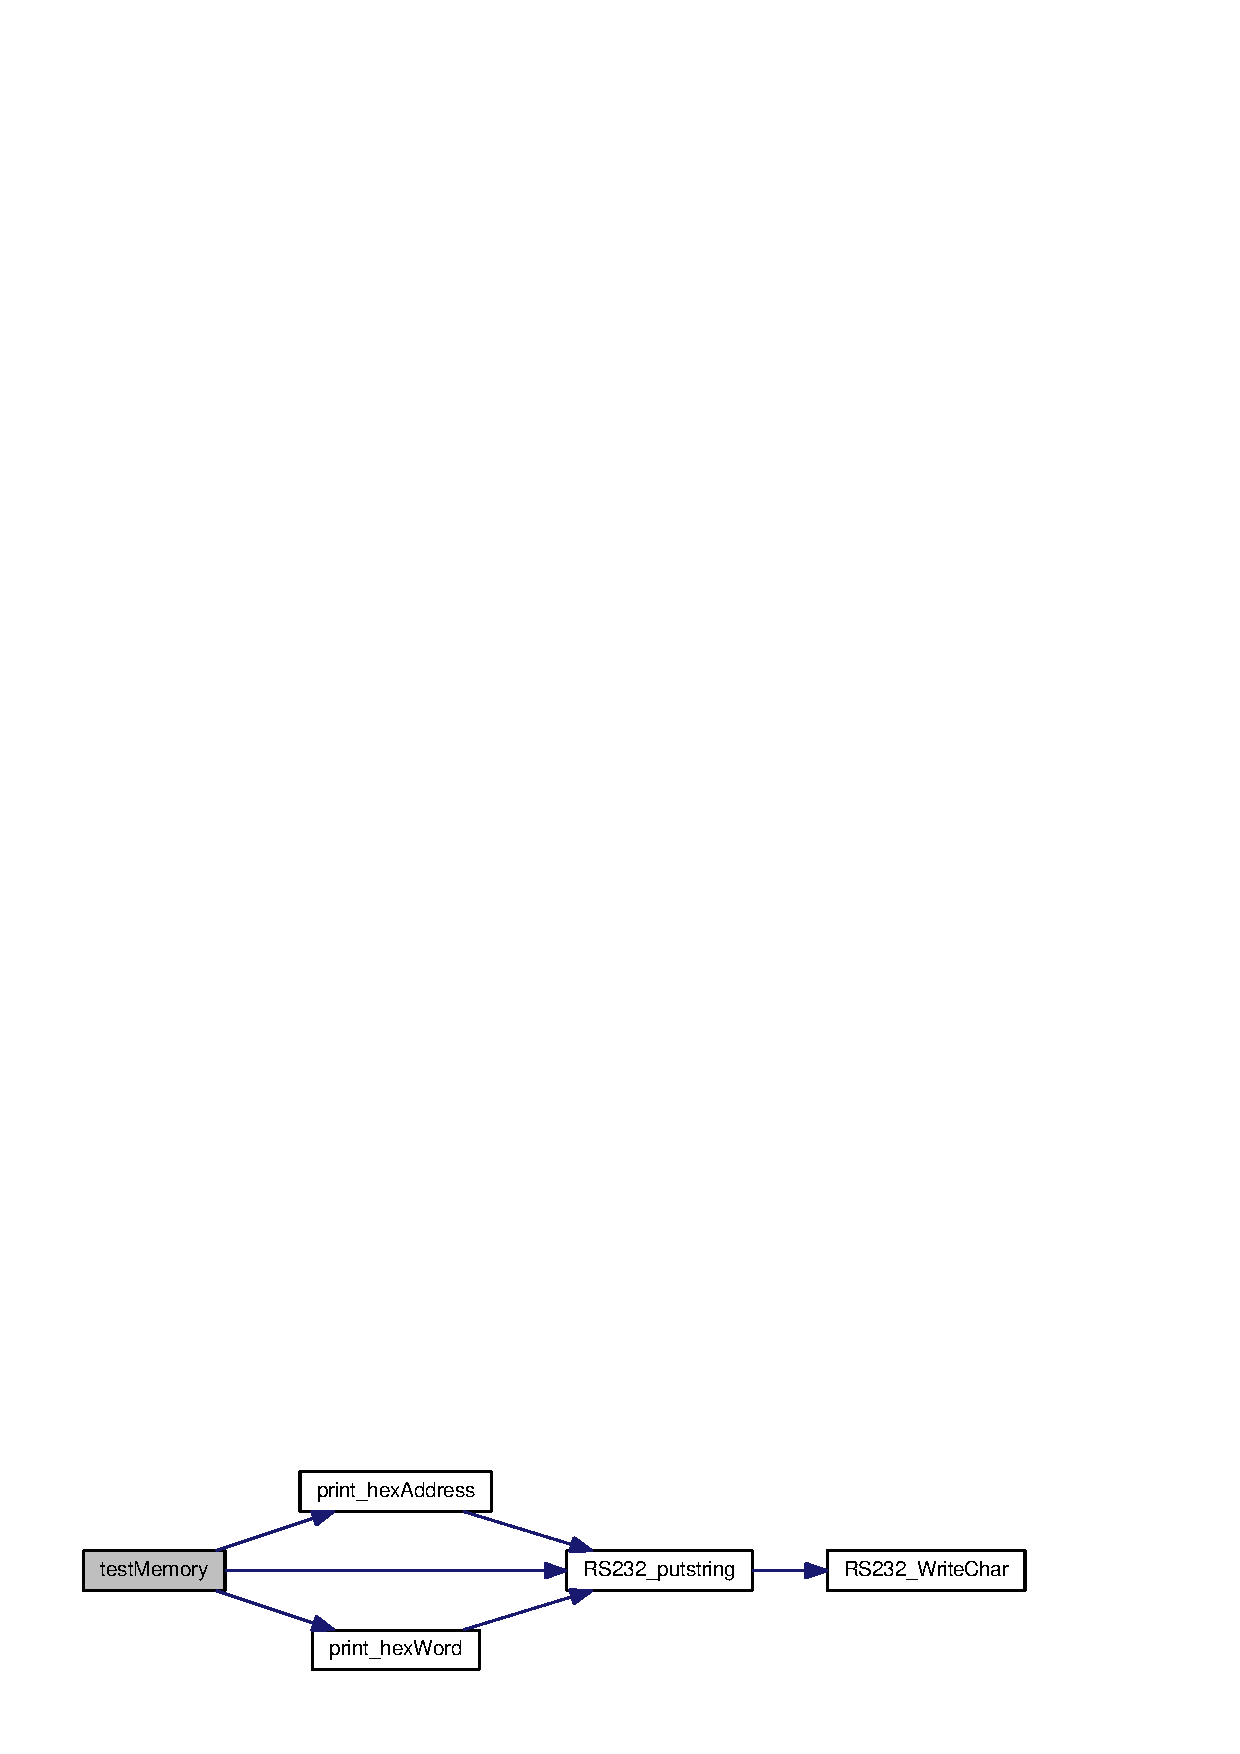
\includegraphics[width=350pt]{my_memory_8h_ae811c849e7999d4868458fffe1f87f8e_cgraph}
\end{center}
\end{figure}


\index{my\+Memory.\+h@{my\+Memory.\+h}!X\+M\+E\+M\+\_\+init@{X\+M\+E\+M\+\_\+init}}
\index{X\+M\+E\+M\+\_\+init@{X\+M\+E\+M\+\_\+init}!my\+Memory.\+h@{my\+Memory.\+h}}
\subsubsection[{X\+M\+E\+M\+\_\+init(void)}]{\setlength{\rightskip}{0pt plus 5cm}void X\+M\+E\+M\+\_\+init (
\begin{DoxyParamCaption}
\item[{void}]{}
\end{DoxyParamCaption}
)}\label{my_memory_8h_aa40171b2238355469afb6141d6f9d612}


Definition at line 113 of file my\+Memory.\+c.


\section{U\+:/\+I\+C\+T/7th\+\_\+semester/bpri2/code/my\+Ethernut/rs485/src/my\+R\+T\+L.c File Reference}
\label{my_r_t_l_8c}\index{U\+:/\+I\+C\+T/7th\+\_\+semester/bpri2/code/my\+Ethernut/rs485/src/my\+R\+T\+L.\+c@{U\+:/\+I\+C\+T/7th\+\_\+semester/bpri2/code/my\+Ethernut/rs485/src/my\+R\+T\+L.\+c}}
{\ttfamily \#include \char`\"{}my\+R\+T\+L.\+h\char`\"{}}\\*
Include dependency graph for my\+R\+T\+L.\+c\+:\nopagebreak
\begin{figure}[H]
\begin{center}
\leavevmode
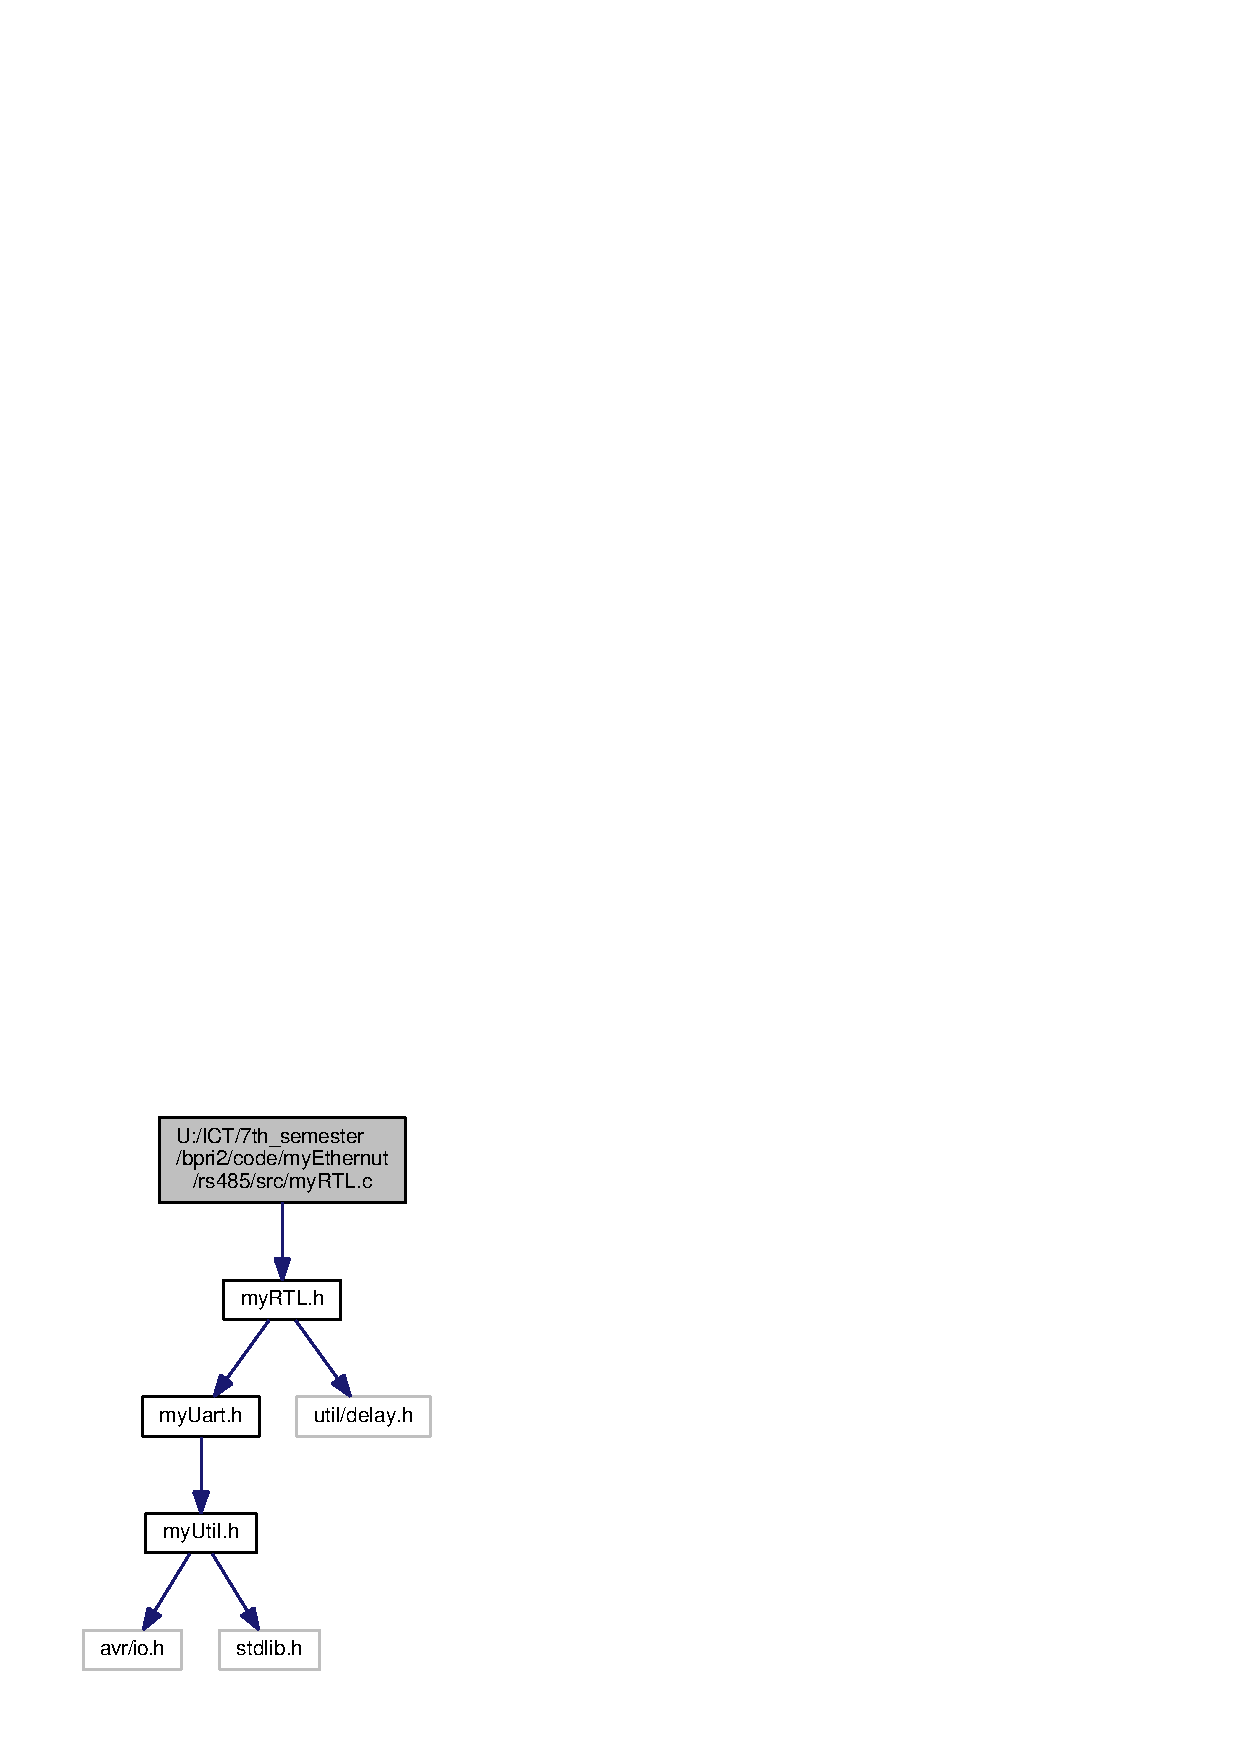
\includegraphics[width=211pt]{my_r_t_l_8c__incl}
\end{center}
\end{figure}
\subsection*{Functions}
\begin{DoxyCompactItemize}
\item 
void {\bf Test\+Realtek} (void)
\item 
{\bf u\+\_\+short} {\bf Test\+External\+Ram} ({\bf u\+\_\+short} first, {\bf u\+\_\+short} last)
\end{DoxyCompactItemize}


\subsection{Function Documentation}
\index{my\+R\+T\+L.\+c@{my\+R\+T\+L.\+c}!Test\+External\+Ram@{Test\+External\+Ram}}
\index{Test\+External\+Ram@{Test\+External\+Ram}!my\+R\+T\+L.\+c@{my\+R\+T\+L.\+c}}
\subsubsection[{Test\+External\+Ram(u\+\_\+short first, u\+\_\+short last)}]{\setlength{\rightskip}{0pt plus 5cm}{\bf u\+\_\+short} Test\+External\+Ram (
\begin{DoxyParamCaption}
\item[{{\bf u\+\_\+short}}]{first, }
\item[{{\bf u\+\_\+short}}]{last}
\end{DoxyParamCaption}
)}\label{my_r_t_l_8c_aae574c84382f7e74ca5d13ddadc8f3db}


Definition at line 78 of file my\+R\+T\+L.\+c.



References print\+\_\+hex\+Byte(), and R\+S232\+\_\+putstring().



Here is the call graph for this function\+:\nopagebreak
\begin{figure}[H]
\begin{center}
\leavevmode
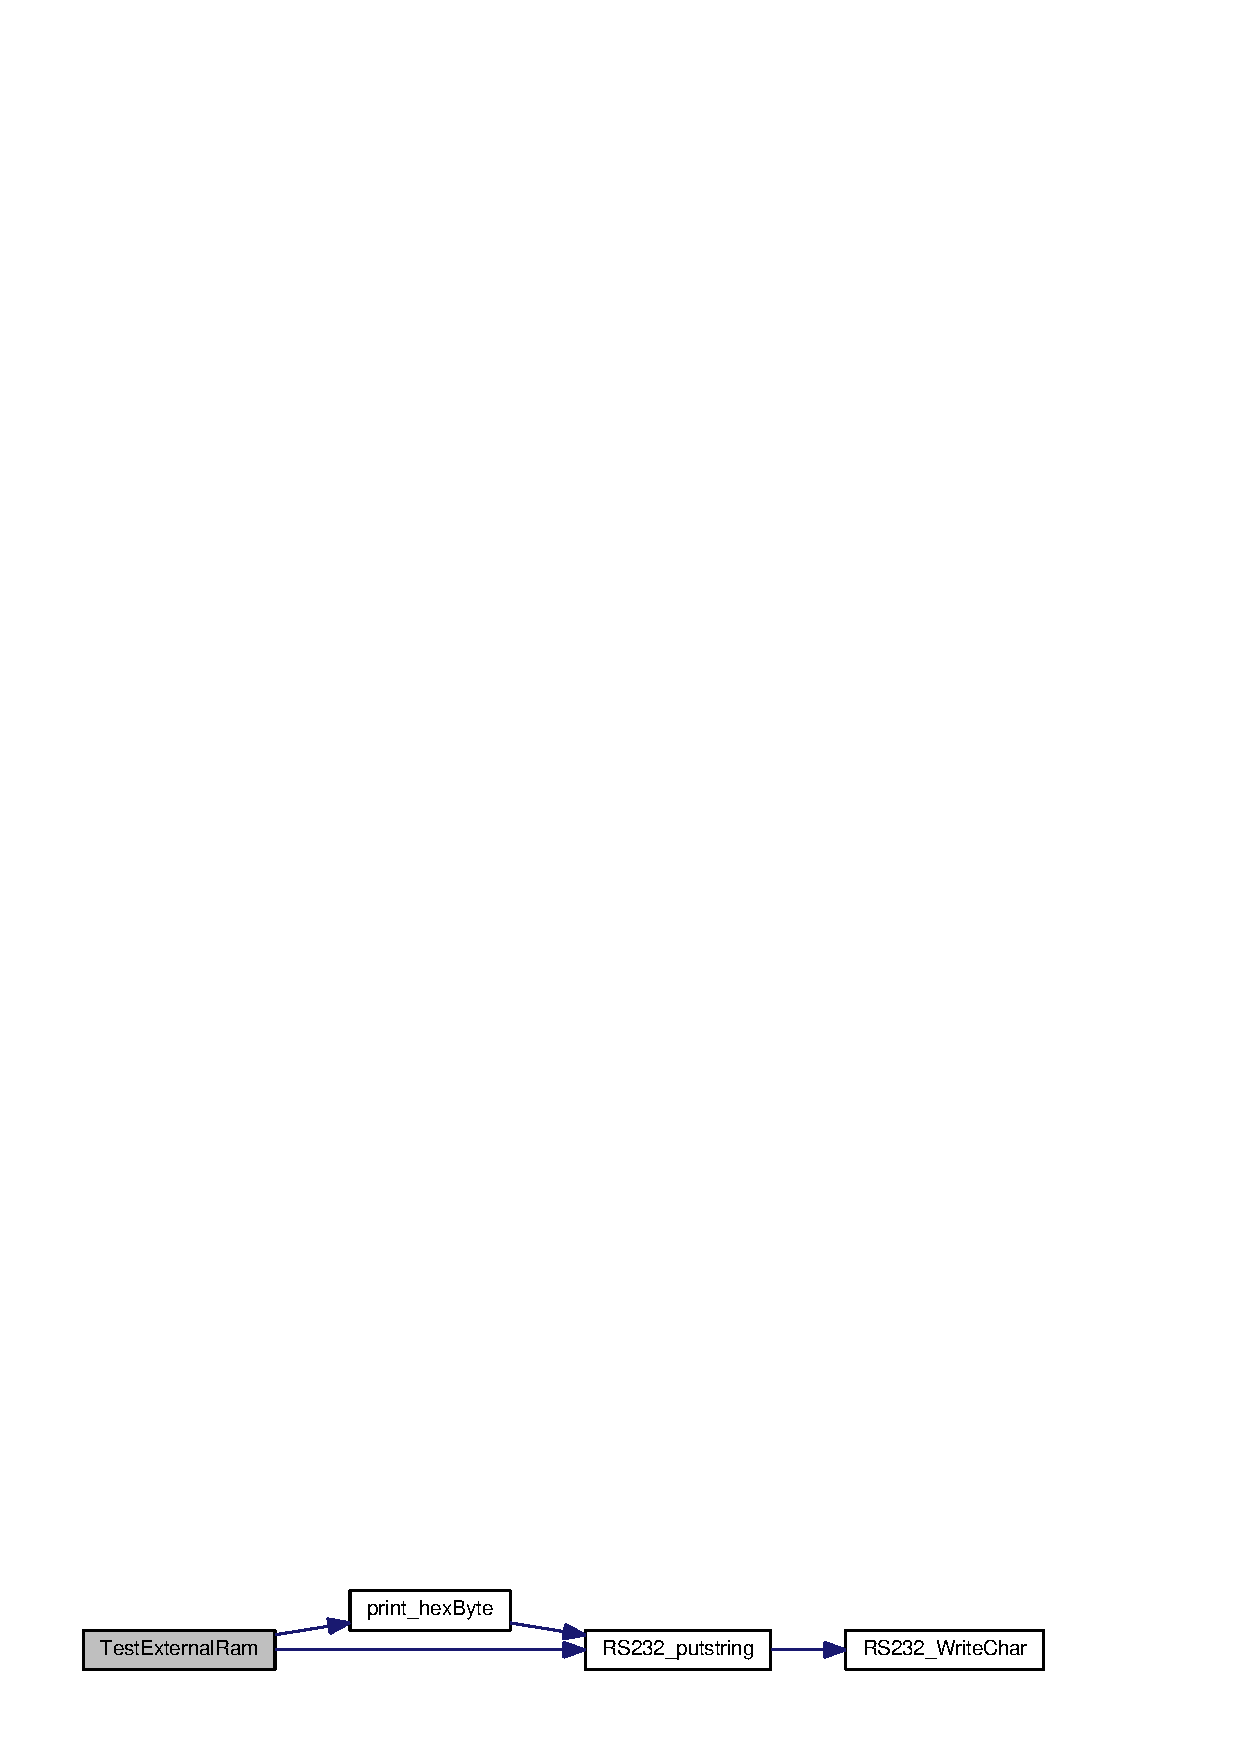
\includegraphics[width=350pt]{my_r_t_l_8c_aae574c84382f7e74ca5d13ddadc8f3db_cgraph}
\end{center}
\end{figure}


\index{my\+R\+T\+L.\+c@{my\+R\+T\+L.\+c}!Test\+Realtek@{Test\+Realtek}}
\index{Test\+Realtek@{Test\+Realtek}!my\+R\+T\+L.\+c@{my\+R\+T\+L.\+c}}
\subsubsection[{Test\+Realtek(void)}]{\setlength{\rightskip}{0pt plus 5cm}void Test\+Realtek (
\begin{DoxyParamCaption}
\item[{void}]{}
\end{DoxyParamCaption}
)}\label{my_r_t_l_8c_a769ab791b25df68a642ef98332c4732f}


Definition at line 5 of file my\+R\+T\+L.\+c.



References print\+\_\+hex\+Word(), and R\+S232\+\_\+putstring().



Here is the call graph for this function\+:\nopagebreak
\begin{figure}[H]
\begin{center}
\leavevmode
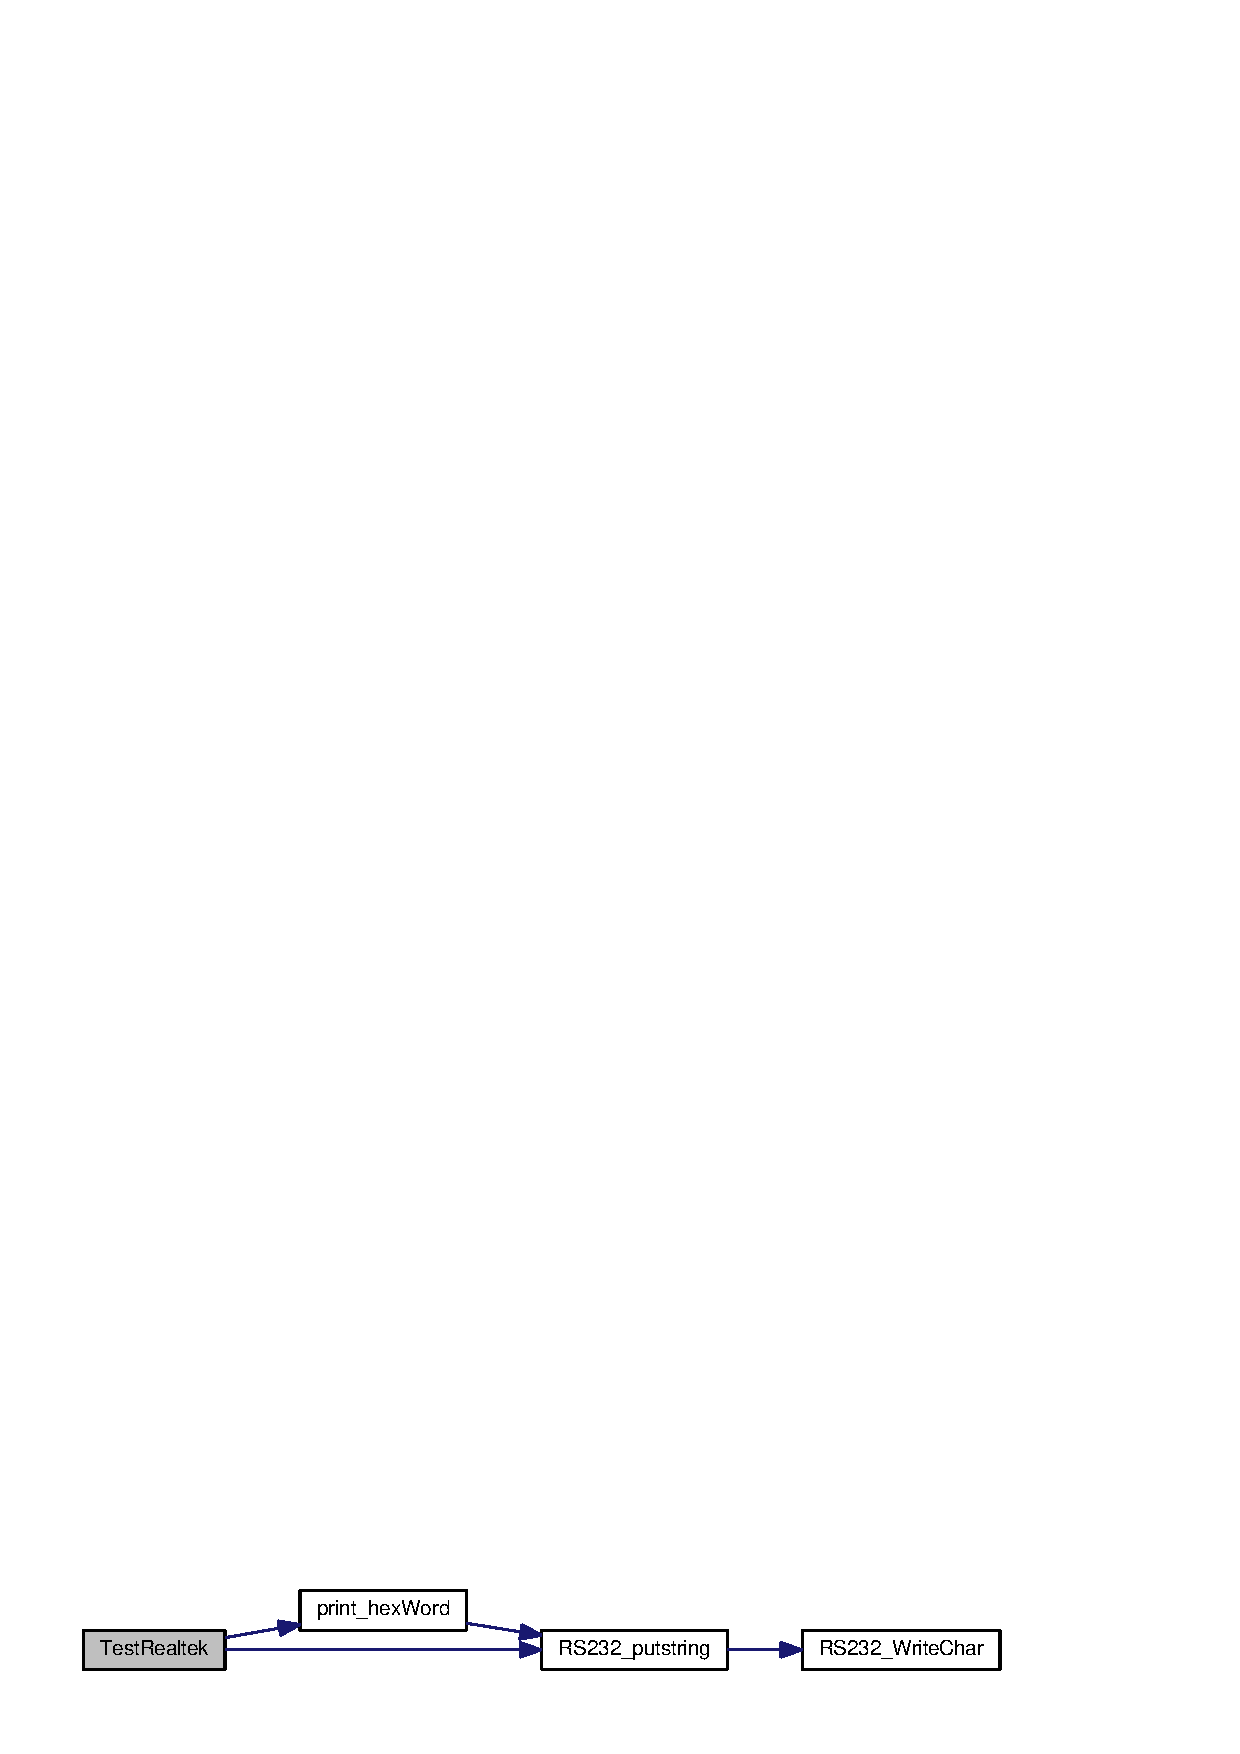
\includegraphics[width=350pt]{my_r_t_l_8c_a769ab791b25df68a642ef98332c4732f_cgraph}
\end{center}
\end{figure}



\section{U\+:/\+I\+C\+T/7th\+\_\+semester/bpri2/code/my\+Ethernut/rs485/src/my\+R\+T\+L.h File Reference}
\label{my_r_t_l_8h}\index{U\+:/\+I\+C\+T/7th\+\_\+semester/bpri2/code/my\+Ethernut/rs485/src/my\+R\+T\+L.\+h@{U\+:/\+I\+C\+T/7th\+\_\+semester/bpri2/code/my\+Ethernut/rs485/src/my\+R\+T\+L.\+h}}
{\ttfamily \#include \char`\"{}my\+Uart.\+h\char`\"{}}\\*
{\ttfamily \#include $<$util/delay.\+h$>$}\\*
Include dependency graph for my\+R\+T\+L.\+h\+:\nopagebreak
\begin{figure}[H]
\begin{center}
\leavevmode
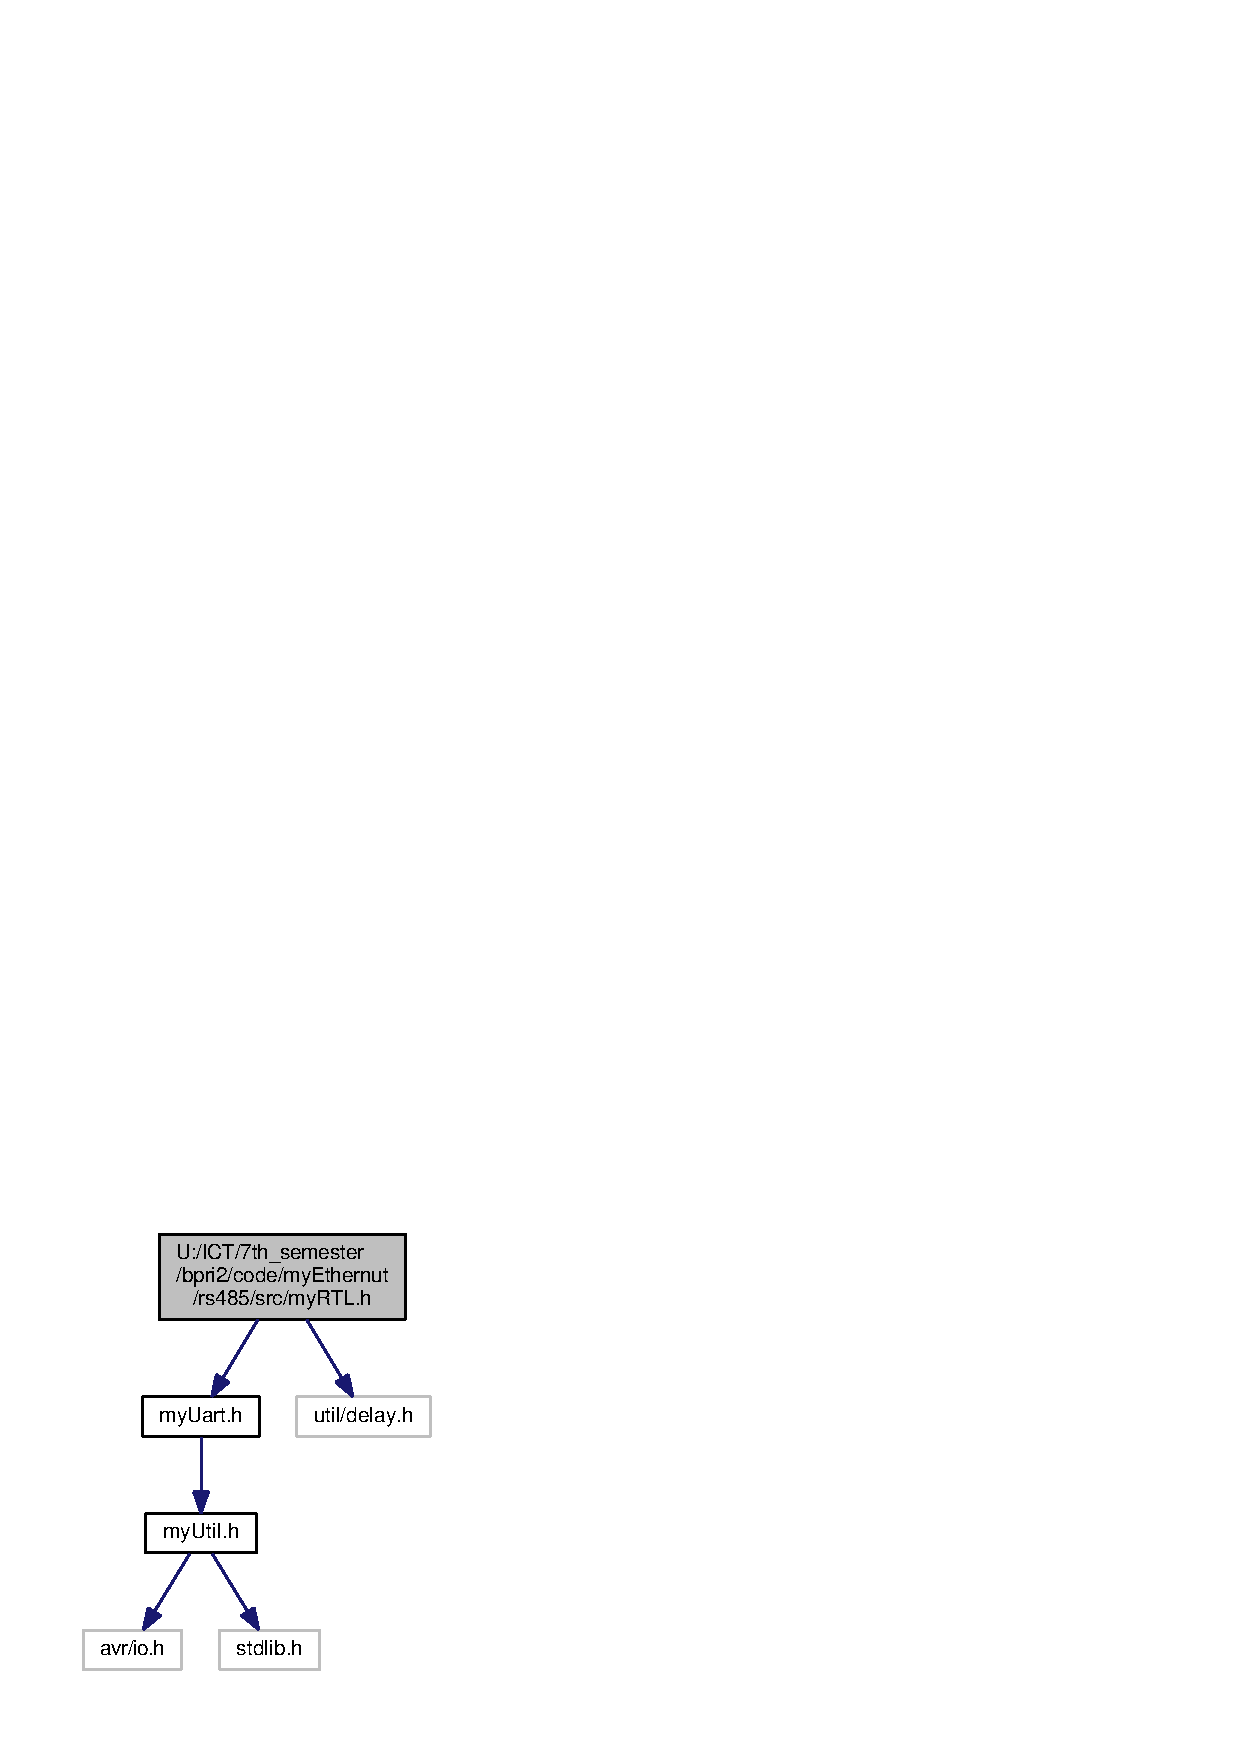
\includegraphics[width=211pt]{my_r_t_l_8h__incl}
\end{center}
\end{figure}
This graph shows which files directly or indirectly include this file\+:\nopagebreak
\begin{figure}[H]
\begin{center}
\leavevmode
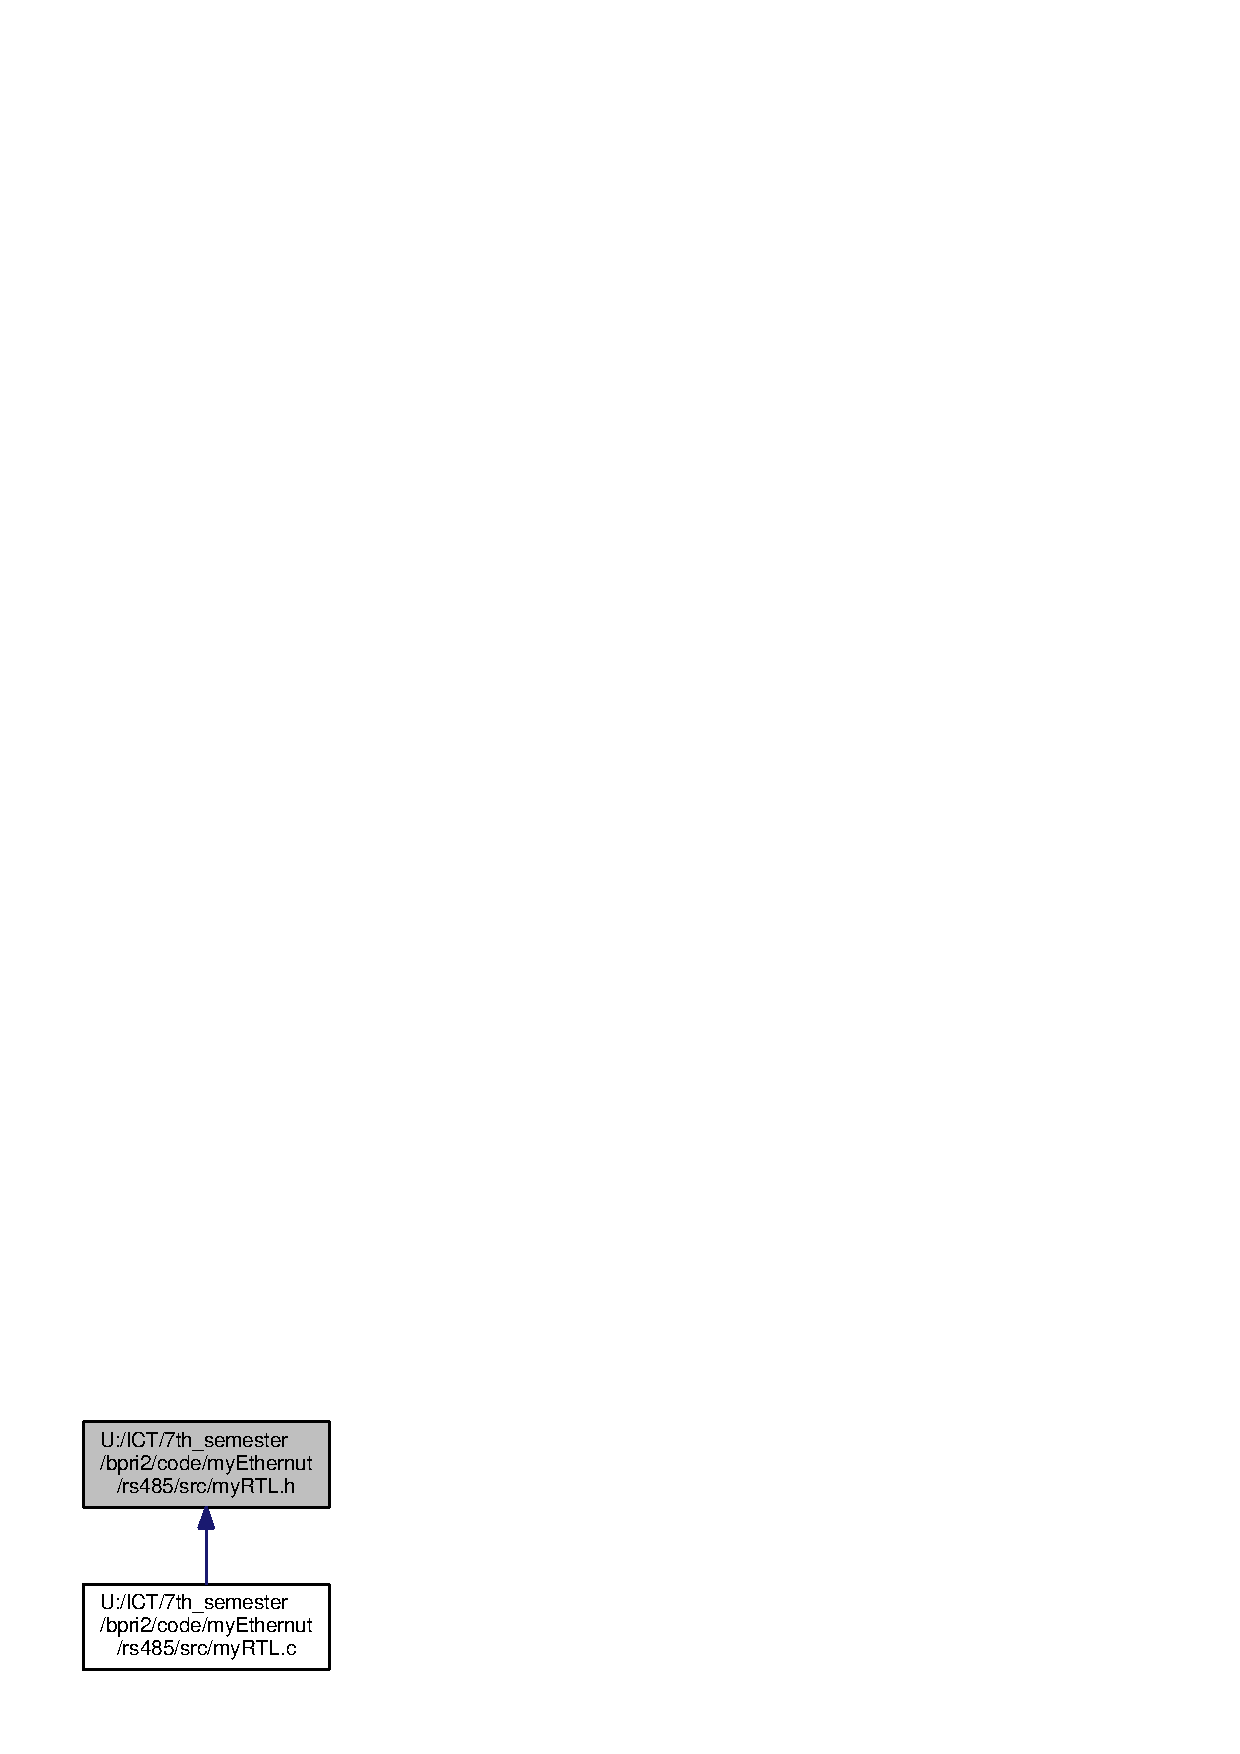
\includegraphics[width=162pt]{my_r_t_l_8h__dep__incl}
\end{center}
\end{figure}
\subsection*{Typedefs}
\begin{DoxyCompactItemize}
\item 
typedef unsigned char {\bf u\+\_\+char}
\item 
typedef unsigned short {\bf u\+\_\+short}
\end{DoxyCompactItemize}
\subsection*{Functions}
\begin{DoxyCompactItemize}
\item 
void {\bf Test\+Realtek} (void)
\item 
{\bf u\+\_\+short} {\bf Test\+External\+Ram} ({\bf u\+\_\+short} first, {\bf u\+\_\+short} last)
\end{DoxyCompactItemize}


\subsection{Typedef Documentation}
\index{my\+R\+T\+L.\+h@{my\+R\+T\+L.\+h}!u\+\_\+char@{u\+\_\+char}}
\index{u\+\_\+char@{u\+\_\+char}!my\+R\+T\+L.\+h@{my\+R\+T\+L.\+h}}
\subsubsection[{u\+\_\+char}]{\setlength{\rightskip}{0pt plus 5cm}typedef unsigned char {\bf u\+\_\+char}}\label{my_r_t_l_8h_ae2b02ed168fc99cff3851603910b1fb6}


Definition at line 10 of file my\+R\+T\+L.\+h.

\index{my\+R\+T\+L.\+h@{my\+R\+T\+L.\+h}!u\+\_\+short@{u\+\_\+short}}
\index{u\+\_\+short@{u\+\_\+short}!my\+R\+T\+L.\+h@{my\+R\+T\+L.\+h}}
\subsubsection[{u\+\_\+short}]{\setlength{\rightskip}{0pt plus 5cm}typedef unsigned short {\bf u\+\_\+short}}\label{my_r_t_l_8h_aa1a19deefc008737e6397f44d983cfd4}


Definition at line 11 of file my\+R\+T\+L.\+h.



\subsection{Function Documentation}
\index{my\+R\+T\+L.\+h@{my\+R\+T\+L.\+h}!Test\+External\+Ram@{Test\+External\+Ram}}
\index{Test\+External\+Ram@{Test\+External\+Ram}!my\+R\+T\+L.\+h@{my\+R\+T\+L.\+h}}
\subsubsection[{Test\+External\+Ram(u\+\_\+short first, u\+\_\+short last)}]{\setlength{\rightskip}{0pt plus 5cm}{\bf u\+\_\+short} Test\+External\+Ram (
\begin{DoxyParamCaption}
\item[{{\bf u\+\_\+short}}]{first, }
\item[{{\bf u\+\_\+short}}]{last}
\end{DoxyParamCaption}
)}\label{my_r_t_l_8h_aae574c84382f7e74ca5d13ddadc8f3db}


Definition at line 78 of file my\+R\+T\+L.\+c.



References print\+\_\+hex\+Byte(), and R\+S232\+\_\+putstring().



Here is the call graph for this function\+:\nopagebreak
\begin{figure}[H]
\begin{center}
\leavevmode
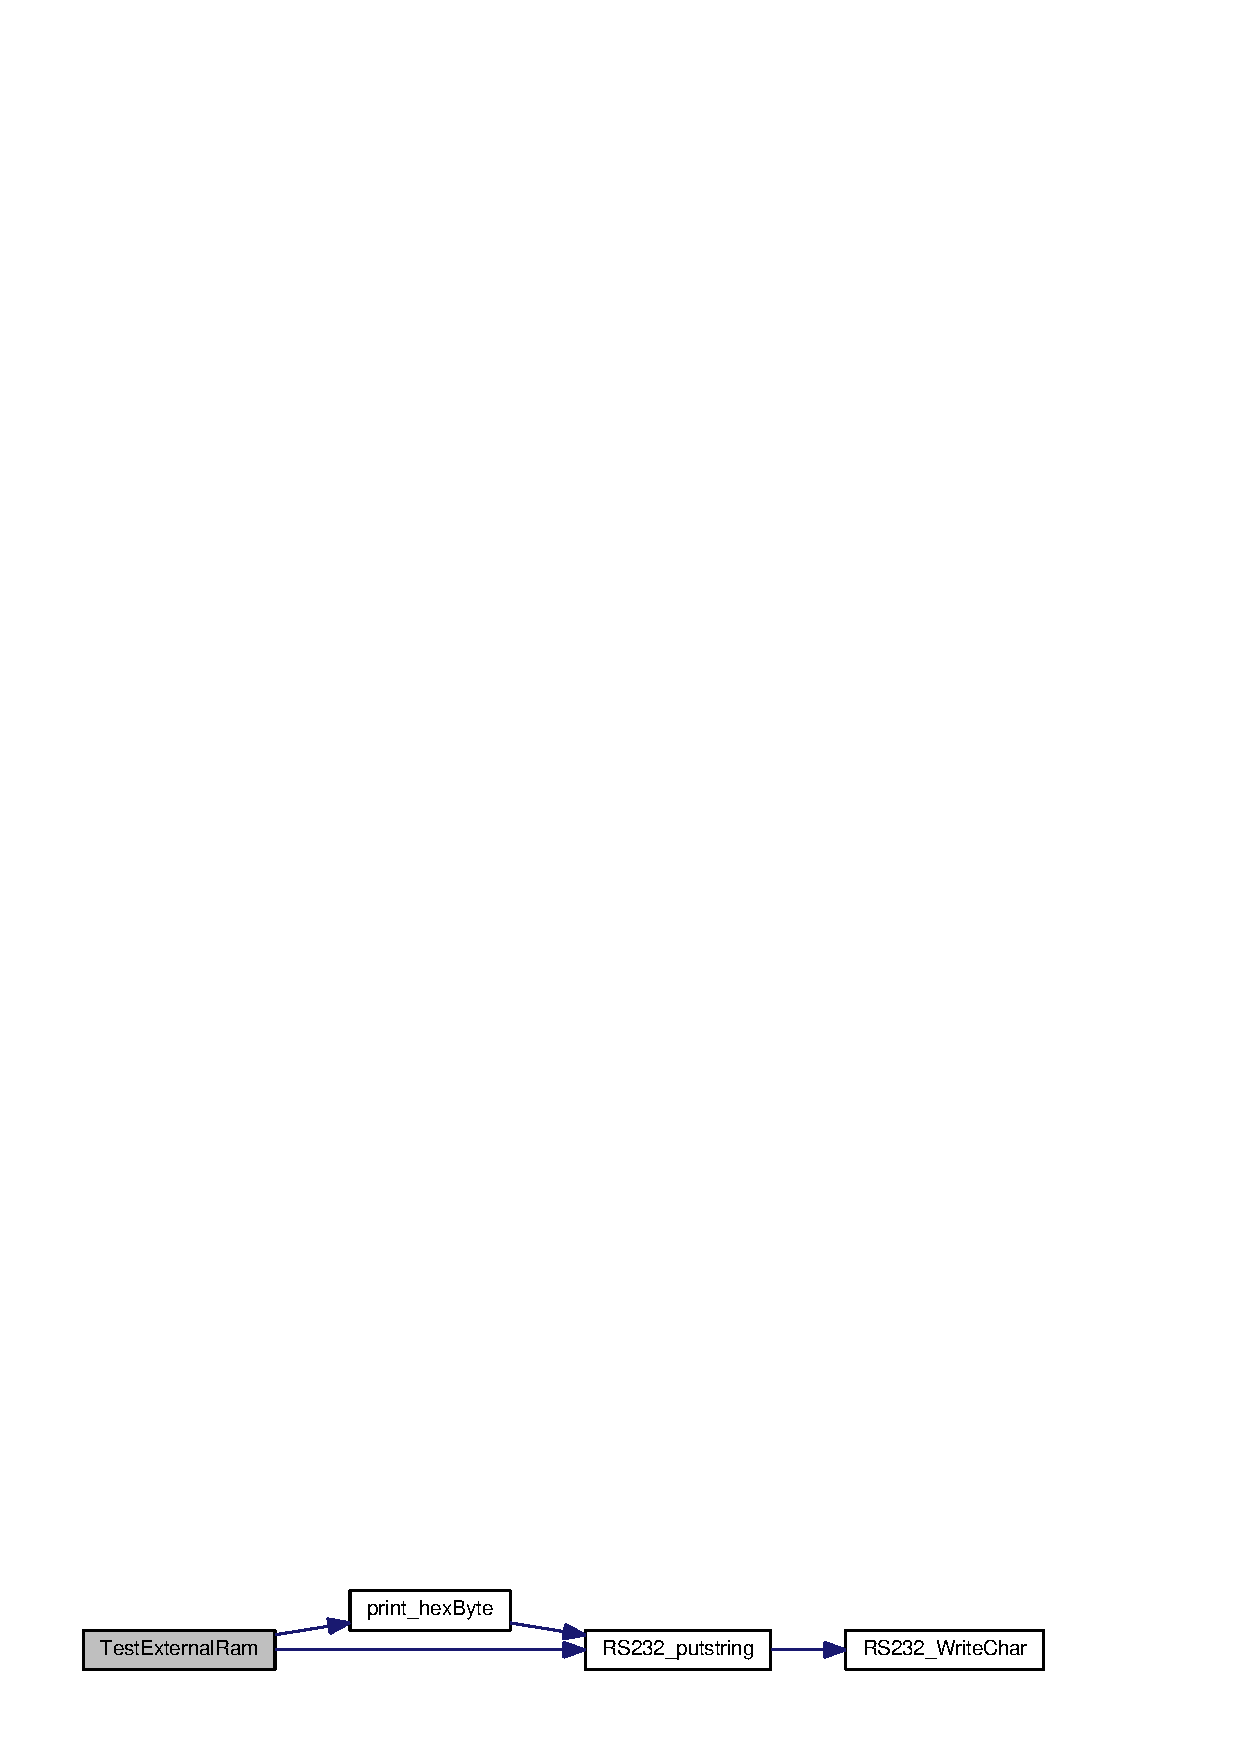
\includegraphics[width=350pt]{my_r_t_l_8h_aae574c84382f7e74ca5d13ddadc8f3db_cgraph}
\end{center}
\end{figure}


\index{my\+R\+T\+L.\+h@{my\+R\+T\+L.\+h}!Test\+Realtek@{Test\+Realtek}}
\index{Test\+Realtek@{Test\+Realtek}!my\+R\+T\+L.\+h@{my\+R\+T\+L.\+h}}
\subsubsection[{Test\+Realtek(void)}]{\setlength{\rightskip}{0pt plus 5cm}void Test\+Realtek (
\begin{DoxyParamCaption}
\item[{void}]{}
\end{DoxyParamCaption}
)}\label{my_r_t_l_8h_a769ab791b25df68a642ef98332c4732f}


Definition at line 5 of file my\+R\+T\+L.\+c.



References print\+\_\+hex\+Word(), and R\+S232\+\_\+putstring().



Here is the call graph for this function\+:\nopagebreak
\begin{figure}[H]
\begin{center}
\leavevmode
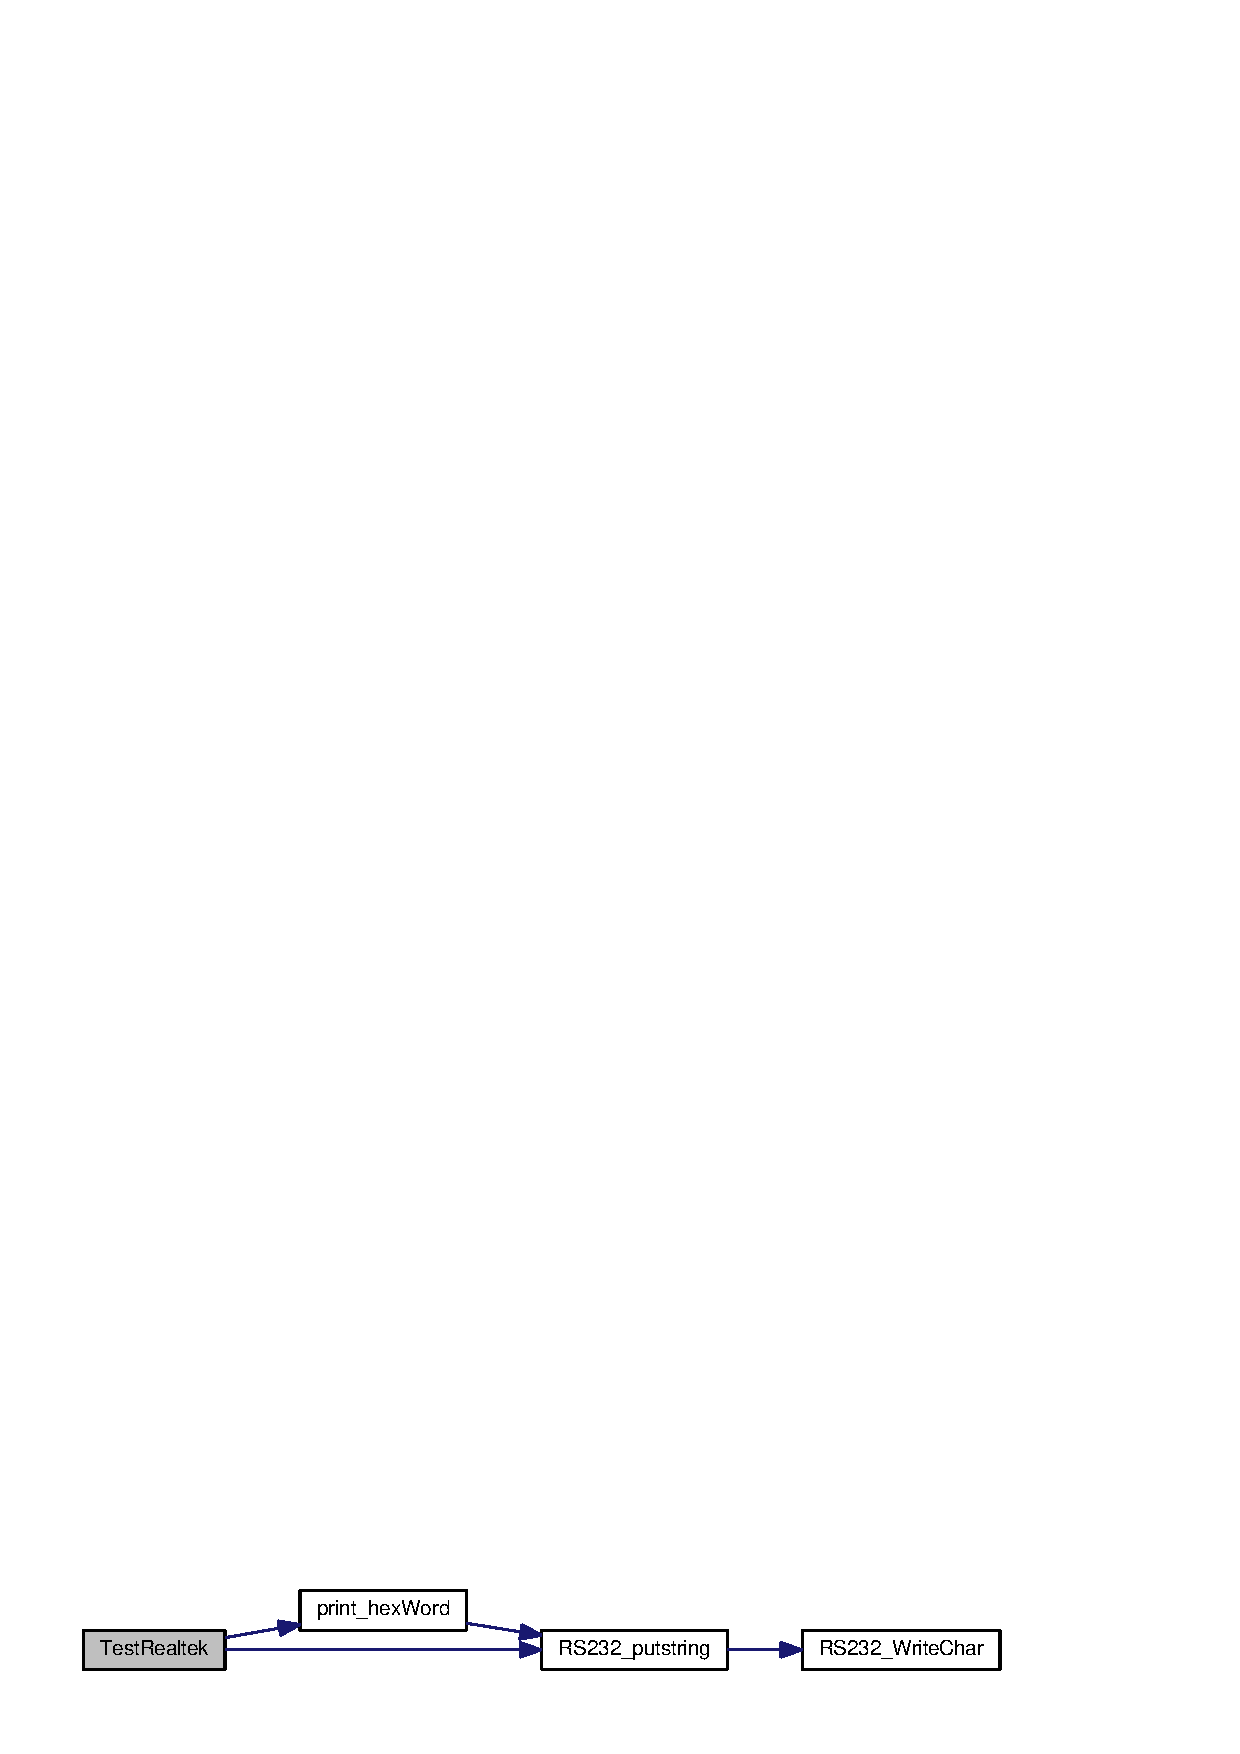
\includegraphics[width=350pt]{my_r_t_l_8h_a769ab791b25df68a642ef98332c4732f_cgraph}
\end{center}
\end{figure}



\section{U\+:/\+I\+C\+T/7th\+\_\+semester/bpri2/code/my\+Ethernut/rs485/src/my\+Trash.c File Reference}
\label{my_trash_8c}\index{U\+:/\+I\+C\+T/7th\+\_\+semester/bpri2/code/my\+Ethernut/rs485/src/my\+Trash.\+c@{U\+:/\+I\+C\+T/7th\+\_\+semester/bpri2/code/my\+Ethernut/rs485/src/my\+Trash.\+c}}

\section{U\+:/\+I\+C\+T/7th\+\_\+semester/bpri2/code/my\+Ethernut/rs485/src/my\+Uart.c File Reference}
\label{my_uart_8c}\index{U\+:/\+I\+C\+T/7th\+\_\+semester/bpri2/code/my\+Ethernut/rs485/src/my\+Uart.\+c@{U\+:/\+I\+C\+T/7th\+\_\+semester/bpri2/code/my\+Ethernut/rs485/src/my\+Uart.\+c}}
{\ttfamily \#include \char`\"{}my\+Uart.\+h\char`\"{}}\\*
Include dependency graph for my\+Uart.\+c\+:\nopagebreak
\begin{figure}[H]
\begin{center}
\leavevmode
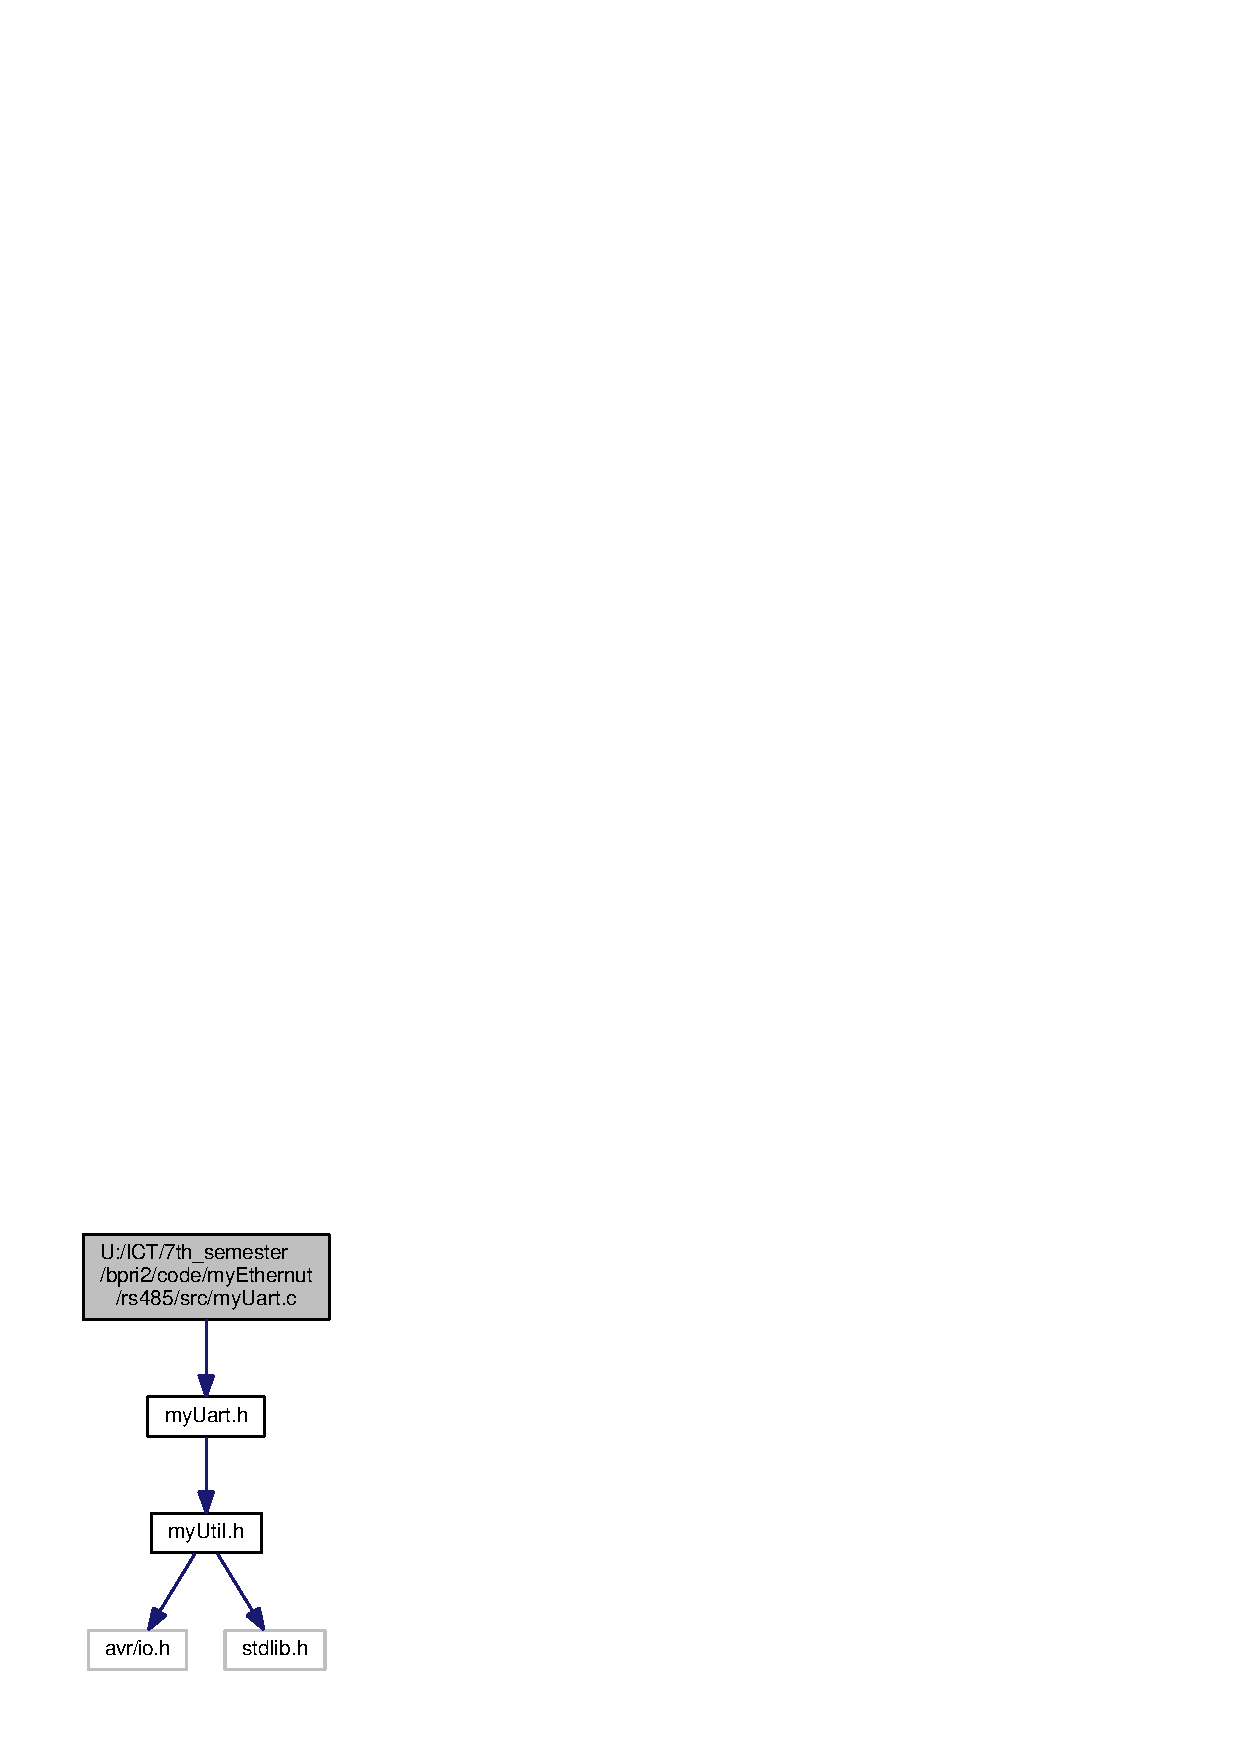
\includegraphics[width=162pt]{my_uart_8c__incl}
\end{center}
\end{figure}
\subsection*{Functions}
\begin{DoxyCompactItemize}
\item 
unsigned char {\bf R\+S232\+\_\+\+Read\+Char} (void)
\item 
unsigned char {\bf R\+S485\+\_\+\+Read\+Char} (void)
\item 
void {\bf R\+S232\+\_\+\+Write\+Char} (unsigned char data)
\item 
void {\bf R\+S485\+\_\+\+Write\+Char} (unsigned char data)
\item 
void {\bf display\+Telegram} (char $\ast$message, uint8\+\_\+t $\ast${\bf my\+Telegram})
\item 
uint8\+\_\+t $\ast$ {\bf R\+S485\+\_\+\+Query\+Telegram} (uint8\+\_\+t $\ast${\bf my\+Telegram})
\item 
void {\bf R\+S232\+\_\+putstring} (char $\ast$String\+Ptr)
\item 
void {\bf R\+S485\+\_\+putstring} (char $\ast$String\+Ptr)
\item 
void {\bf R\+S232\+\_\+init} (uint32\+\_\+t baudrate)
\item 
void {\bf R\+S485\+\_\+init} (uint32\+\_\+t baudrate)
\end{DoxyCompactItemize}


\subsection{Function Documentation}
\index{my\+Uart.\+c@{my\+Uart.\+c}!display\+Telegram@{display\+Telegram}}
\index{display\+Telegram@{display\+Telegram}!my\+Uart.\+c@{my\+Uart.\+c}}
\subsubsection[{display\+Telegram(char $\ast$message, uint8\+\_\+t $\ast$my\+Telegram)}]{\setlength{\rightskip}{0pt plus 5cm}void display\+Telegram (
\begin{DoxyParamCaption}
\item[{char $\ast$}]{message, }
\item[{uint8\+\_\+t $\ast$}]{my\+Telegram}
\end{DoxyParamCaption}
)}\label{my_uart_8c_abb3edba44fb4fb37ad1aa38cce413c3a}


Definition at line 39 of file my\+Uart.\+c.



References print\+\_\+hex\+Byte(), and R\+S232\+\_\+putstring().



Here is the call graph for this function\+:\nopagebreak
\begin{figure}[H]
\begin{center}
\leavevmode
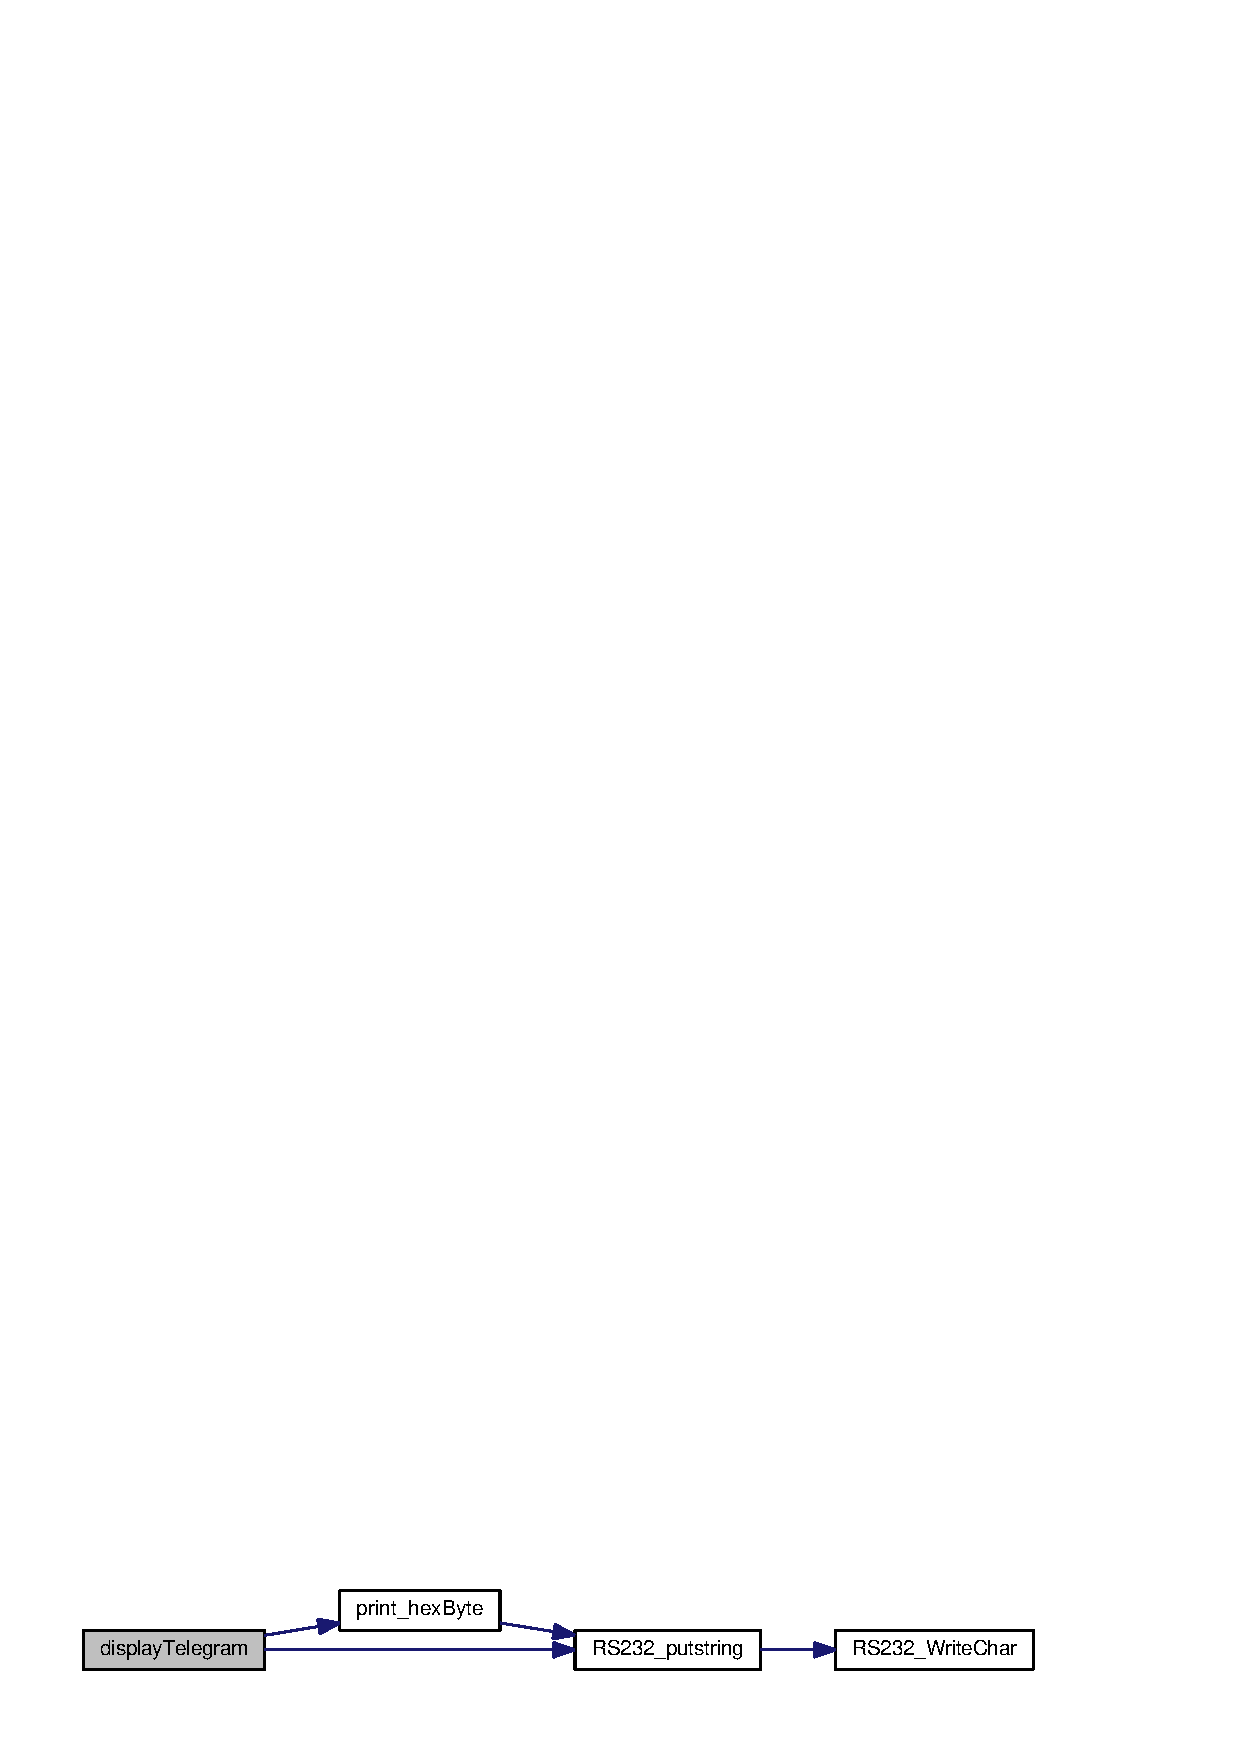
\includegraphics[width=350pt]{my_uart_8c_abb3edba44fb4fb37ad1aa38cce413c3a_cgraph}
\end{center}
\end{figure}


\index{my\+Uart.\+c@{my\+Uart.\+c}!R\+S232\+\_\+init@{R\+S232\+\_\+init}}
\index{R\+S232\+\_\+init@{R\+S232\+\_\+init}!my\+Uart.\+c@{my\+Uart.\+c}}
\subsubsection[{R\+S232\+\_\+init(uint32\+\_\+t baudrate)}]{\setlength{\rightskip}{0pt plus 5cm}void R\+S232\+\_\+init (
\begin{DoxyParamCaption}
\item[{uint32\+\_\+t}]{baudrate}
\end{DoxyParamCaption}
)}\label{my_uart_8c_a06c2a1060a933565013c7e5977139244}


Definition at line 92 of file my\+Uart.\+c.



References F\+\_\+\+C\+P\+U.



Referenced by main().

\index{my\+Uart.\+c@{my\+Uart.\+c}!R\+S232\+\_\+putstring@{R\+S232\+\_\+putstring}}
\index{R\+S232\+\_\+putstring@{R\+S232\+\_\+putstring}!my\+Uart.\+c@{my\+Uart.\+c}}
\subsubsection[{R\+S232\+\_\+putstring(char $\ast$\+String\+Ptr)}]{\setlength{\rightskip}{0pt plus 5cm}void R\+S232\+\_\+putstring (
\begin{DoxyParamCaption}
\item[{char $\ast$}]{String\+Ptr}
\end{DoxyParamCaption}
)}\label{my_uart_8c_a60eaeaa21312415e8b5c05f5376f3541}


Definition at line 77 of file my\+Uart.\+c.



References R\+S232\+\_\+\+Write\+Char().



Referenced by deb\+\_\+print(), display\+Telegram(), main(), print\+\_\+bin\+Byte(), print\+\_\+hex\+Address(), print\+\_\+hex\+Byte(), print\+\_\+hex\+Word(), read\+R\+T\+L\+Memory(), Test\+External\+Ram(), test\+Memory(), and Test\+Realtek().



Here is the call graph for this function\+:\nopagebreak
\begin{figure}[H]
\begin{center}
\leavevmode
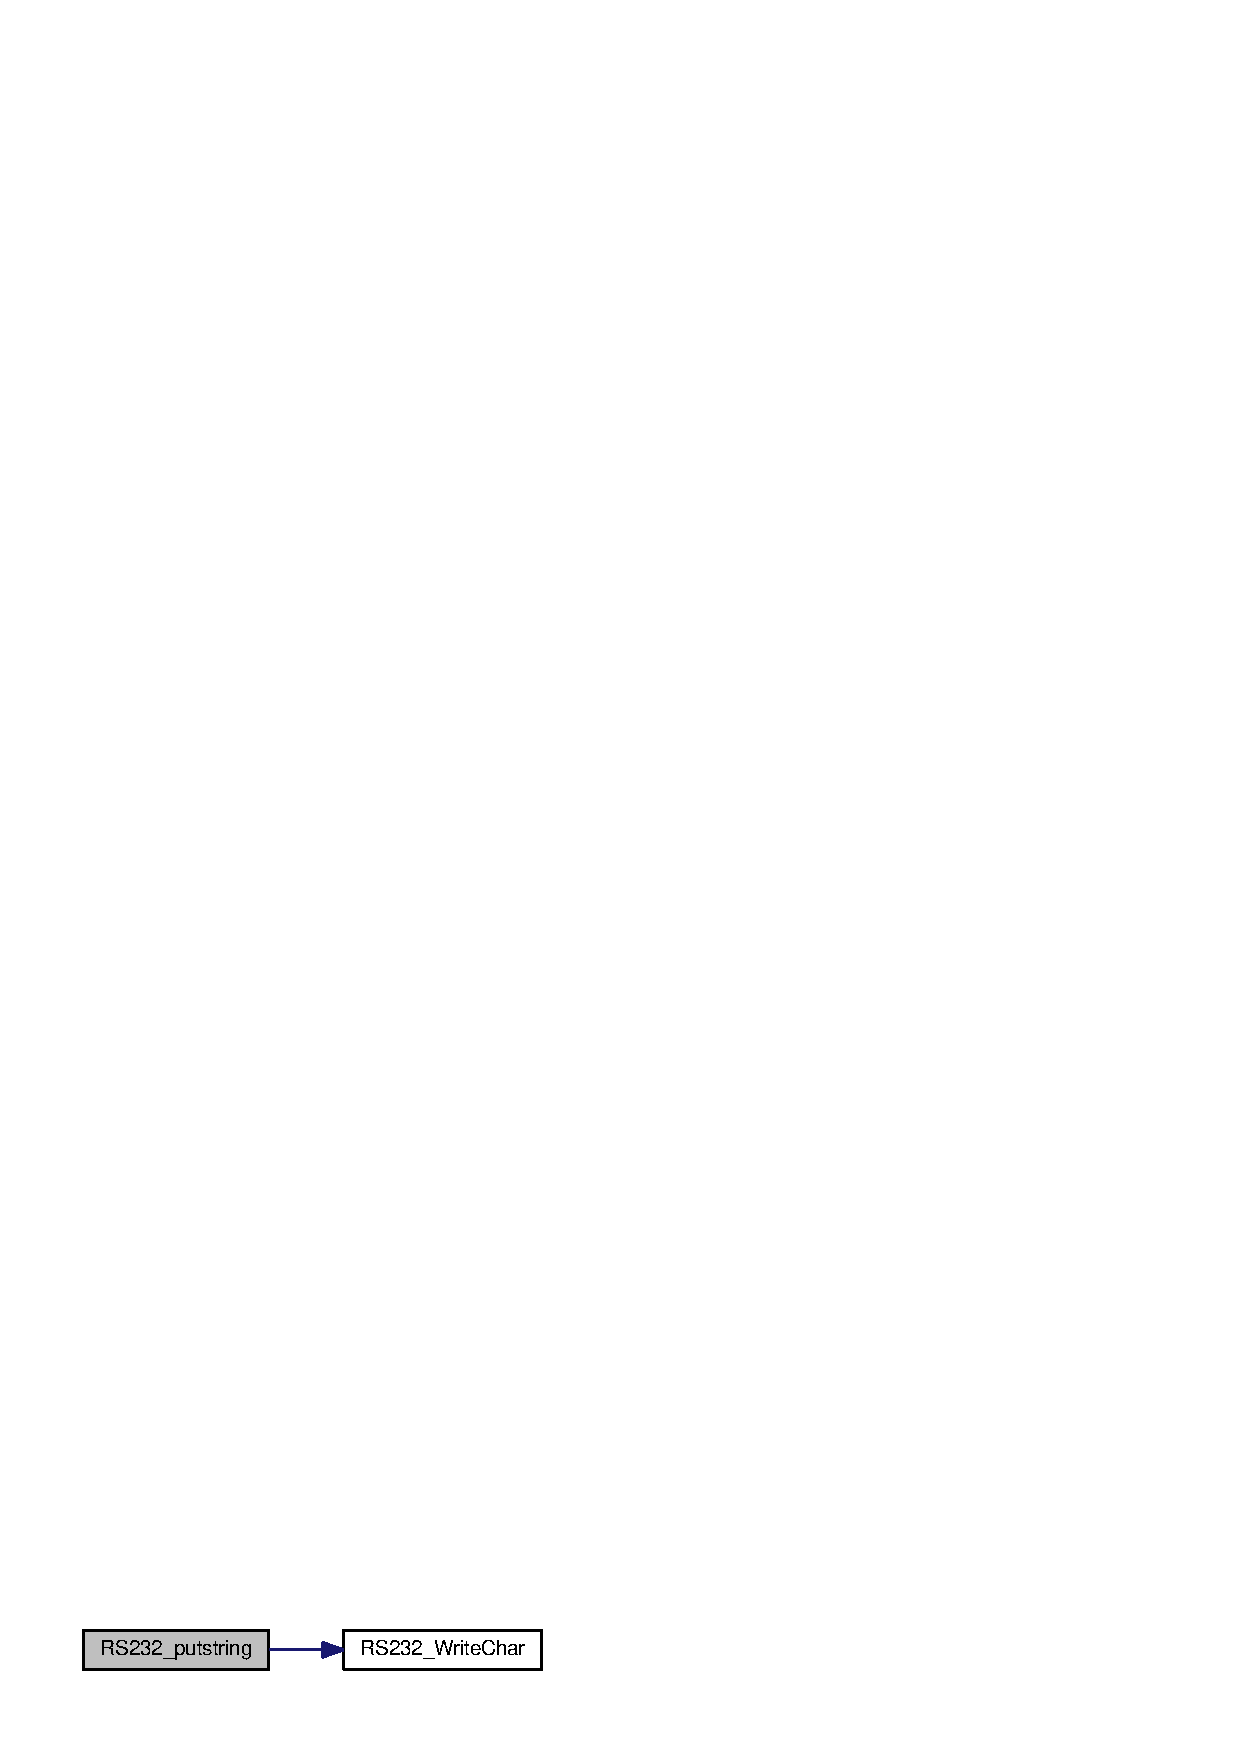
\includegraphics[width=264pt]{my_uart_8c_a60eaeaa21312415e8b5c05f5376f3541_cgraph}
\end{center}
\end{figure}


\index{my\+Uart.\+c@{my\+Uart.\+c}!R\+S232\+\_\+\+Read\+Char@{R\+S232\+\_\+\+Read\+Char}}
\index{R\+S232\+\_\+\+Read\+Char@{R\+S232\+\_\+\+Read\+Char}!my\+Uart.\+c@{my\+Uart.\+c}}
\subsubsection[{R\+S232\+\_\+\+Read\+Char(void)}]{\setlength{\rightskip}{0pt plus 5cm}unsigned char R\+S232\+\_\+\+Read\+Char (
\begin{DoxyParamCaption}
\item[{void}]{}
\end{DoxyParamCaption}
)}\label{my_uart_8c_a50356f8980826894751733073e37ec41}


Definition at line 6 of file my\+Uart.\+c.

\index{my\+Uart.\+c@{my\+Uart.\+c}!R\+S232\+\_\+\+Write\+Char@{R\+S232\+\_\+\+Write\+Char}}
\index{R\+S232\+\_\+\+Write\+Char@{R\+S232\+\_\+\+Write\+Char}!my\+Uart.\+c@{my\+Uart.\+c}}
\subsubsection[{R\+S232\+\_\+\+Write\+Char(unsigned char data)}]{\setlength{\rightskip}{0pt plus 5cm}void R\+S232\+\_\+\+Write\+Char (
\begin{DoxyParamCaption}
\item[{unsigned char}]{data}
\end{DoxyParamCaption}
)}\label{my_uart_8c_a1a99be79a25c05250ff2eca4cbbf9fc5}


Definition at line 24 of file my\+Uart.\+c.



Referenced by print\+\_\+bin\+Byte(), and R\+S232\+\_\+putstring().

\index{my\+Uart.\+c@{my\+Uart.\+c}!R\+S485\+\_\+init@{R\+S485\+\_\+init}}
\index{R\+S485\+\_\+init@{R\+S485\+\_\+init}!my\+Uart.\+c@{my\+Uart.\+c}}
\subsubsection[{R\+S485\+\_\+init(uint32\+\_\+t baudrate)}]{\setlength{\rightskip}{0pt plus 5cm}void R\+S485\+\_\+init (
\begin{DoxyParamCaption}
\item[{uint32\+\_\+t}]{baudrate}
\end{DoxyParamCaption}
)}\label{my_uart_8c_a27f5340823874f42a318aab1e8b4ed50}


Definition at line 103 of file my\+Uart.\+c.



References F\+\_\+\+C\+P\+U.



Referenced by main().

\index{my\+Uart.\+c@{my\+Uart.\+c}!R\+S485\+\_\+putstring@{R\+S485\+\_\+putstring}}
\index{R\+S485\+\_\+putstring@{R\+S485\+\_\+putstring}!my\+Uart.\+c@{my\+Uart.\+c}}
\subsubsection[{R\+S485\+\_\+putstring(char $\ast$\+String\+Ptr)}]{\setlength{\rightskip}{0pt plus 5cm}void R\+S485\+\_\+putstring (
\begin{DoxyParamCaption}
\item[{char $\ast$}]{String\+Ptr}
\end{DoxyParamCaption}
)}\label{my_uart_8c_accde78cd49a35a1dbb5100640334492b}


Definition at line 84 of file my\+Uart.\+c.



References R\+S485\+\_\+\+Write\+Char().



Here is the call graph for this function\+:\nopagebreak
\begin{figure}[H]
\begin{center}
\leavevmode
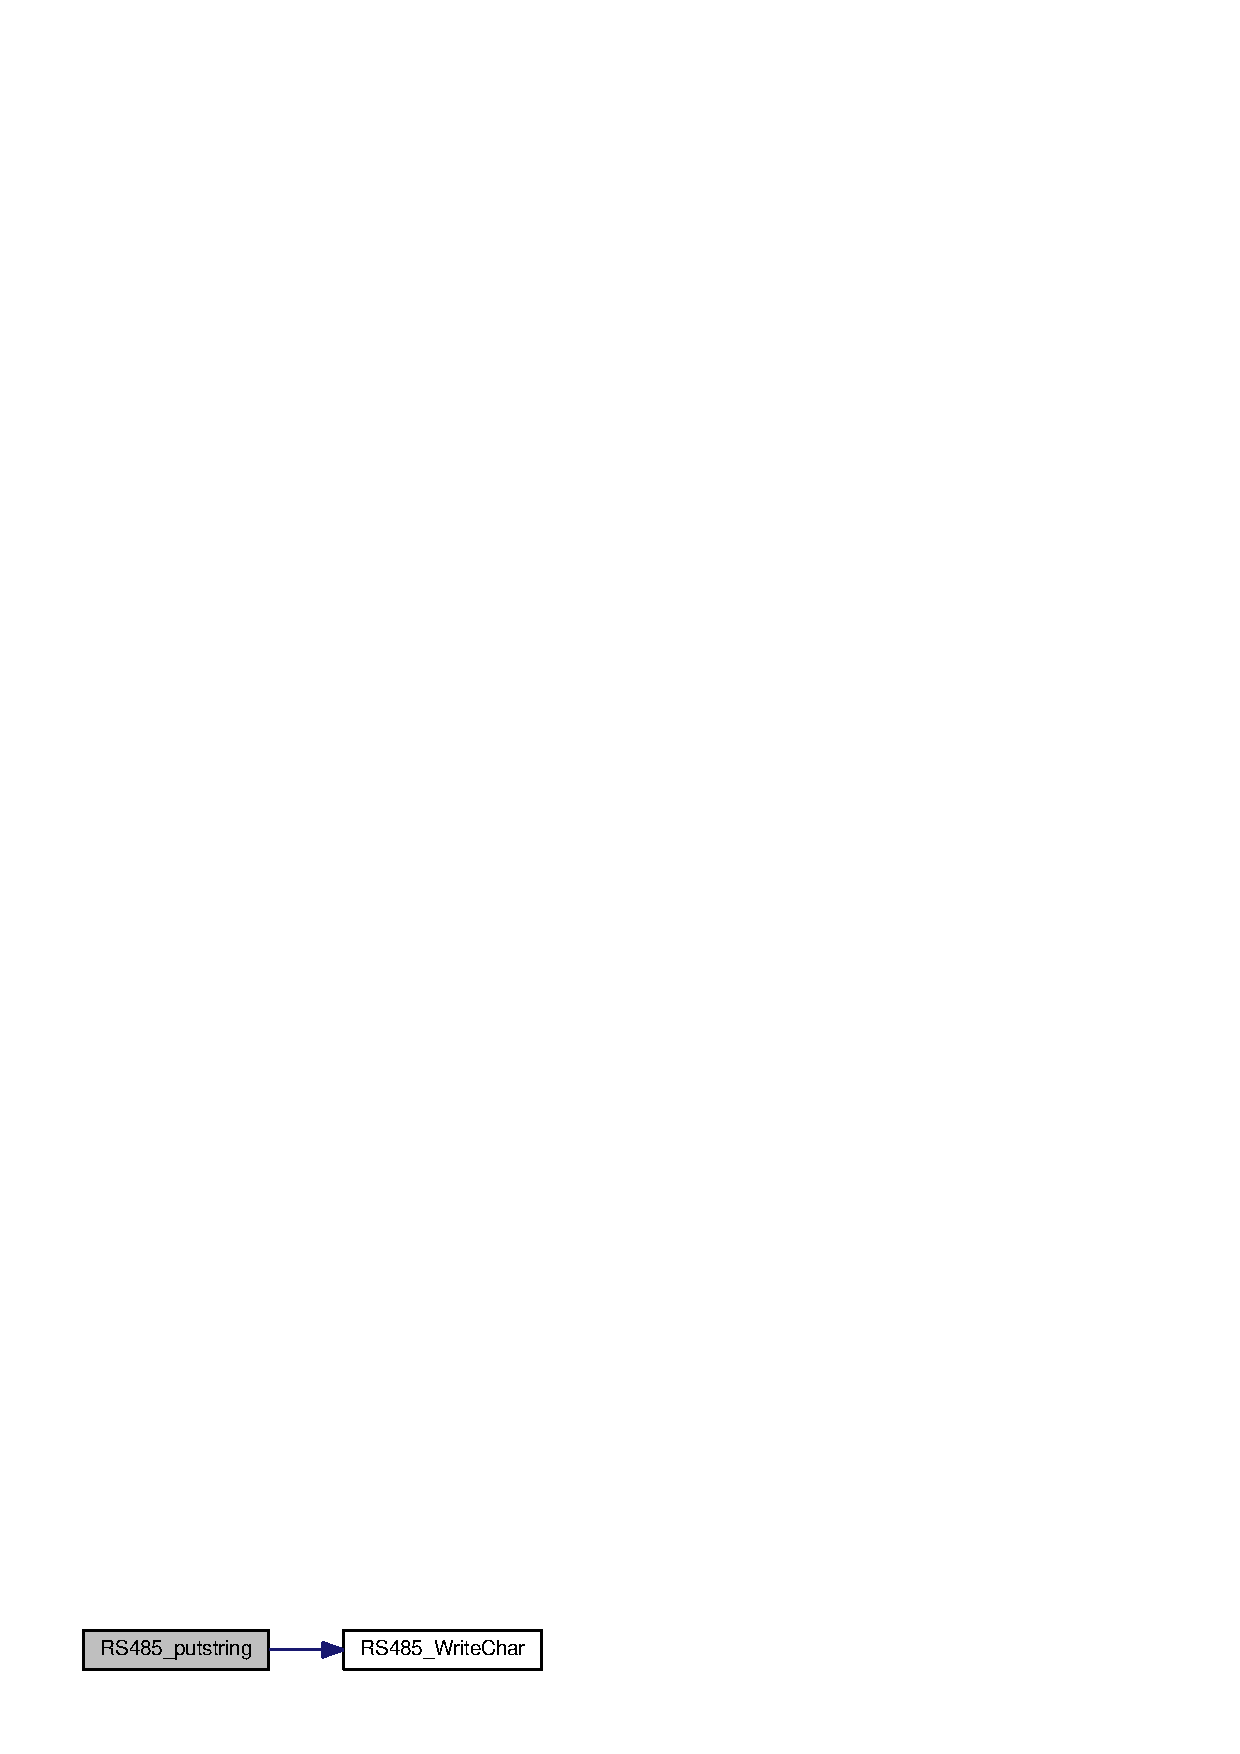
\includegraphics[width=264pt]{my_uart_8c_accde78cd49a35a1dbb5100640334492b_cgraph}
\end{center}
\end{figure}


\index{my\+Uart.\+c@{my\+Uart.\+c}!R\+S485\+\_\+\+Query\+Telegram@{R\+S485\+\_\+\+Query\+Telegram}}
\index{R\+S485\+\_\+\+Query\+Telegram@{R\+S485\+\_\+\+Query\+Telegram}!my\+Uart.\+c@{my\+Uart.\+c}}
\subsubsection[{R\+S485\+\_\+\+Query\+Telegram(uint8\+\_\+t $\ast$my\+Telegram)}]{\setlength{\rightskip}{0pt plus 5cm}uint8\+\_\+t$\ast$ R\+S485\+\_\+\+Query\+Telegram (
\begin{DoxyParamCaption}
\item[{uint8\+\_\+t $\ast$}]{my\+Telegram}
\end{DoxyParamCaption}
)}\label{my_uart_8c_a9b1299202b28a668b8039f538539efb1}


Definition at line 52 of file my\+Uart.\+c.



References my\+Telegram, R\+S485\+\_\+\+Read\+Char(), and R\+S485\+\_\+\+Write\+Char().



Referenced by get\+Value().



Here is the call graph for this function\+:\nopagebreak
\begin{figure}[H]
\begin{center}
\leavevmode
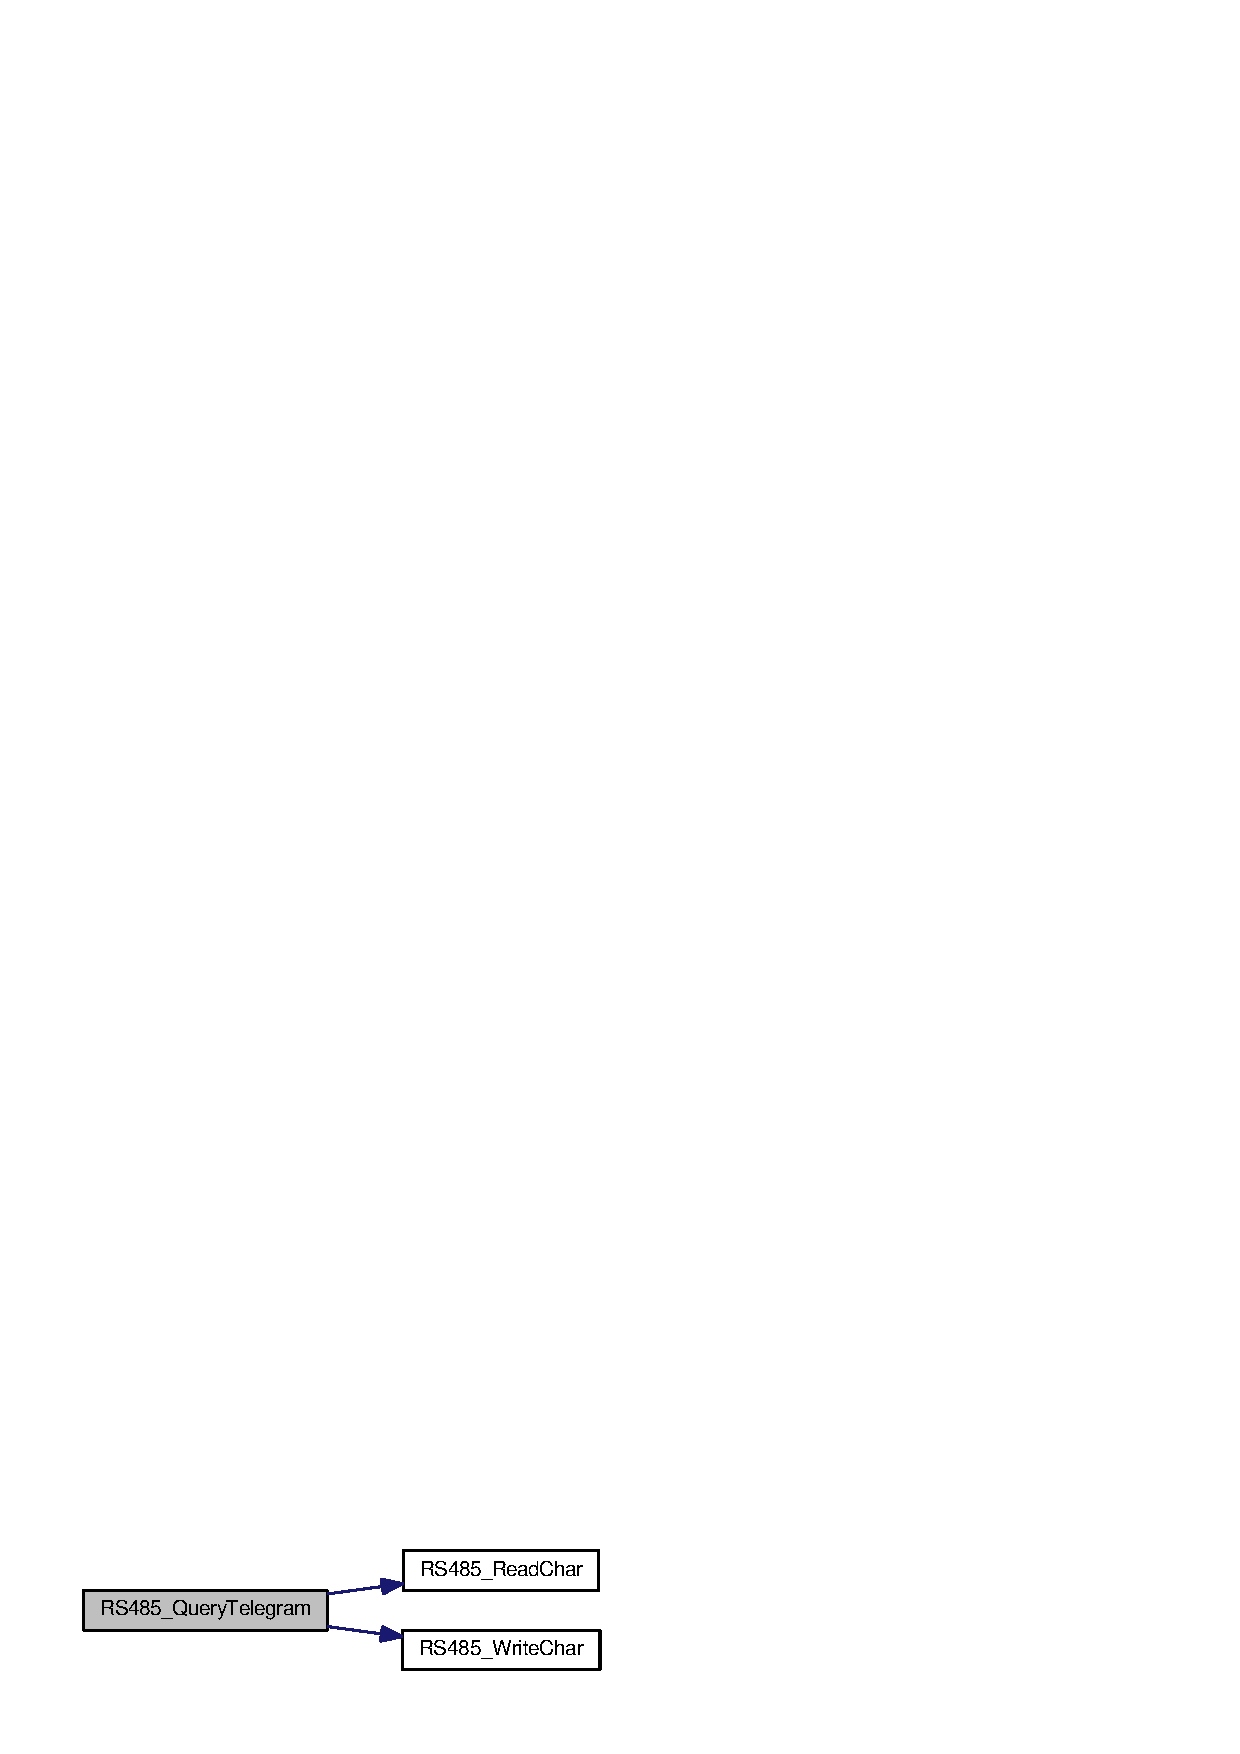
\includegraphics[width=292pt]{my_uart_8c_a9b1299202b28a668b8039f538539efb1_cgraph}
\end{center}
\end{figure}


\index{my\+Uart.\+c@{my\+Uart.\+c}!R\+S485\+\_\+\+Read\+Char@{R\+S485\+\_\+\+Read\+Char}}
\index{R\+S485\+\_\+\+Read\+Char@{R\+S485\+\_\+\+Read\+Char}!my\+Uart.\+c@{my\+Uart.\+c}}
\subsubsection[{R\+S485\+\_\+\+Read\+Char(void)}]{\setlength{\rightskip}{0pt plus 5cm}unsigned char R\+S485\+\_\+\+Read\+Char (
\begin{DoxyParamCaption}
\item[{void}]{}
\end{DoxyParamCaption}
)}\label{my_uart_8c_ab56f53b4e7d6fe7165cdef32270c7a39}


Definition at line 14 of file my\+Uart.\+c.



Referenced by R\+S485\+\_\+\+Query\+Telegram().

\index{my\+Uart.\+c@{my\+Uart.\+c}!R\+S485\+\_\+\+Write\+Char@{R\+S485\+\_\+\+Write\+Char}}
\index{R\+S485\+\_\+\+Write\+Char@{R\+S485\+\_\+\+Write\+Char}!my\+Uart.\+c@{my\+Uart.\+c}}
\subsubsection[{R\+S485\+\_\+\+Write\+Char(unsigned char data)}]{\setlength{\rightskip}{0pt plus 5cm}void R\+S485\+\_\+\+Write\+Char (
\begin{DoxyParamCaption}
\item[{unsigned char}]{data}
\end{DoxyParamCaption}
)}\label{my_uart_8c_aeb49100d16c0c1b323128896ed286558}


Definition at line 32 of file my\+Uart.\+c.



Referenced by R\+S485\+\_\+putstring(), and R\+S485\+\_\+\+Query\+Telegram().


\section{U\+:/\+I\+C\+T/7th\+\_\+semester/bpri2/code/my\+Ethernut/rs485/src/my\+Uart.h File Reference}
\label{my_uart_8h}\index{U\+:/\+I\+C\+T/7th\+\_\+semester/bpri2/code/my\+Ethernut/rs485/src/my\+Uart.\+h@{U\+:/\+I\+C\+T/7th\+\_\+semester/bpri2/code/my\+Ethernut/rs485/src/my\+Uart.\+h}}
{\ttfamily \#include \char`\"{}my\+Util.\+h\char`\"{}}\\*
Include dependency graph for my\+Uart.\+h\+:\nopagebreak
\begin{figure}[H]
\begin{center}
\leavevmode
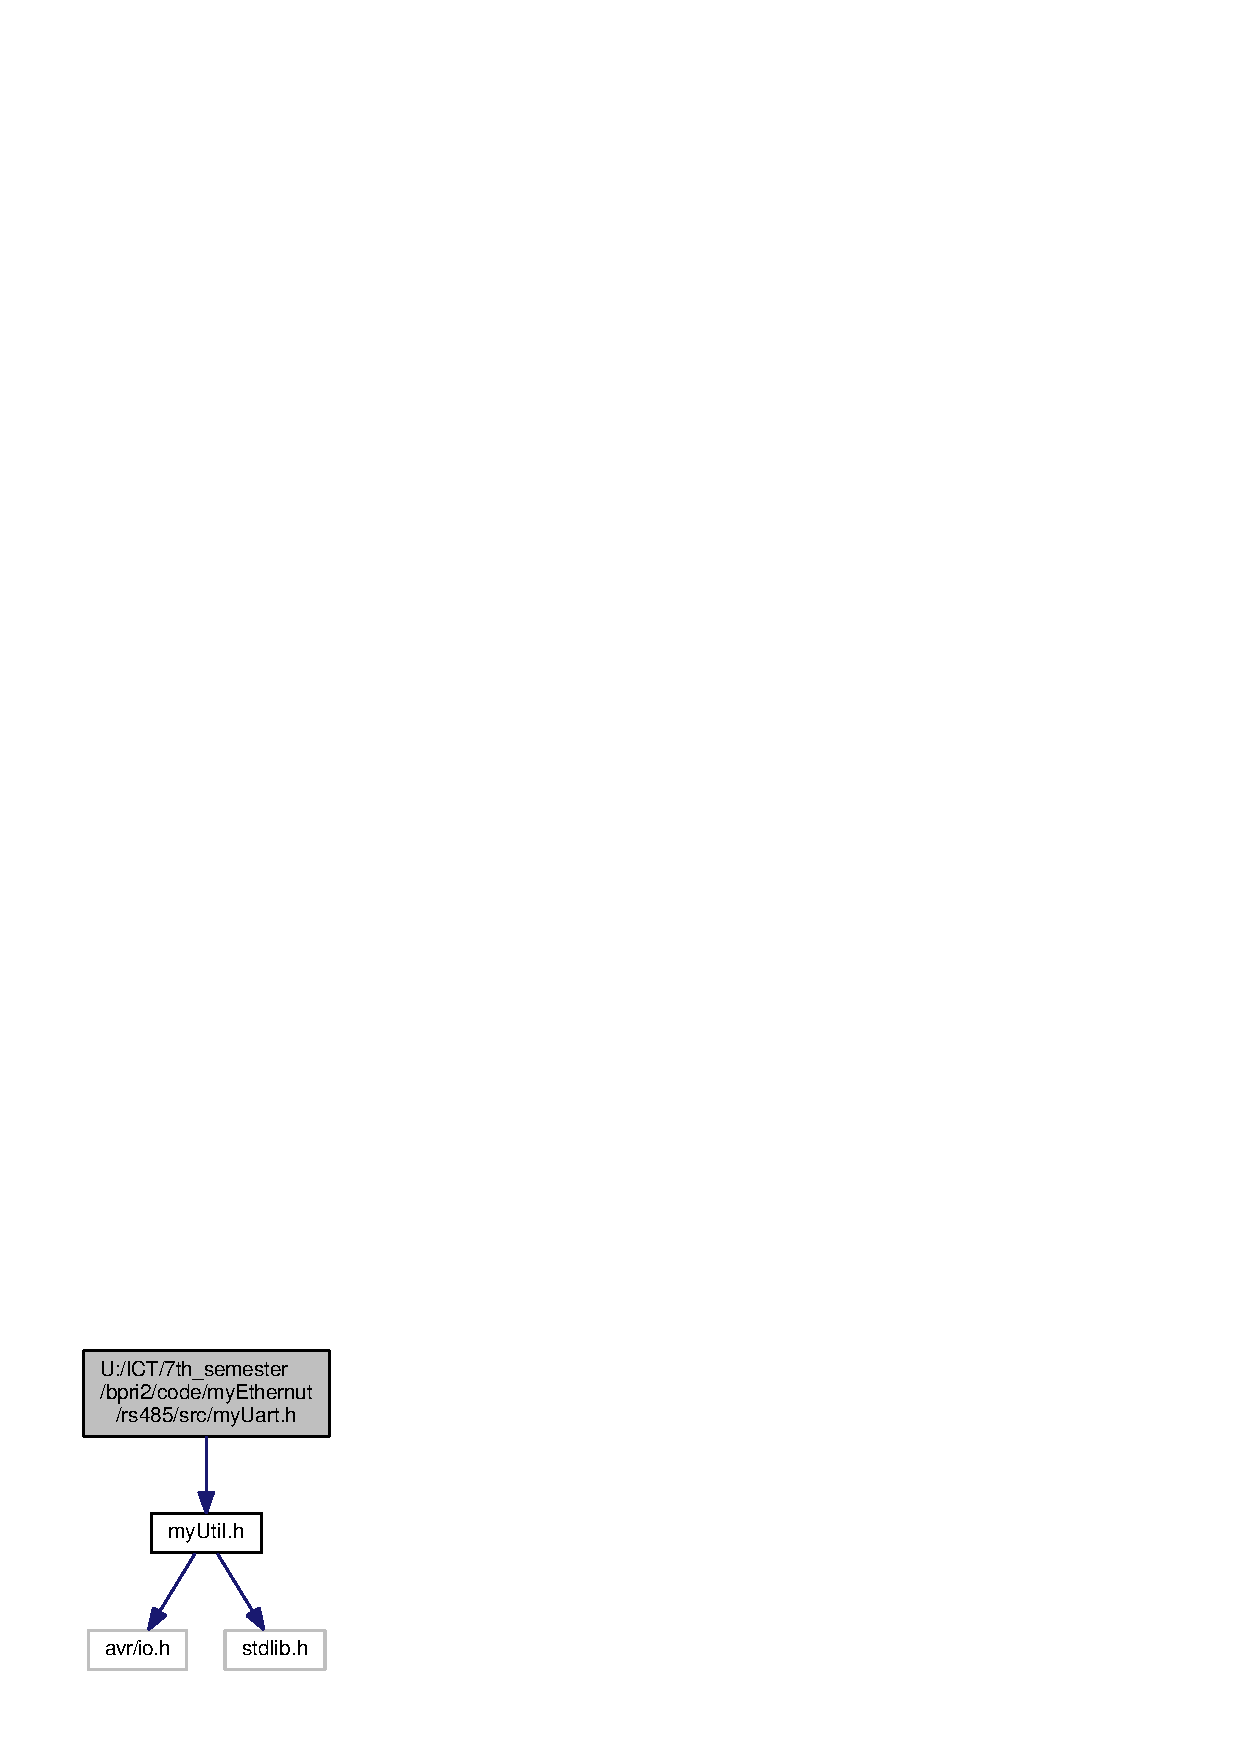
\includegraphics[width=162pt]{my_uart_8h__incl}
\end{center}
\end{figure}
This graph shows which files directly or indirectly include this file\+:\nopagebreak
\begin{figure}[H]
\begin{center}
\leavevmode
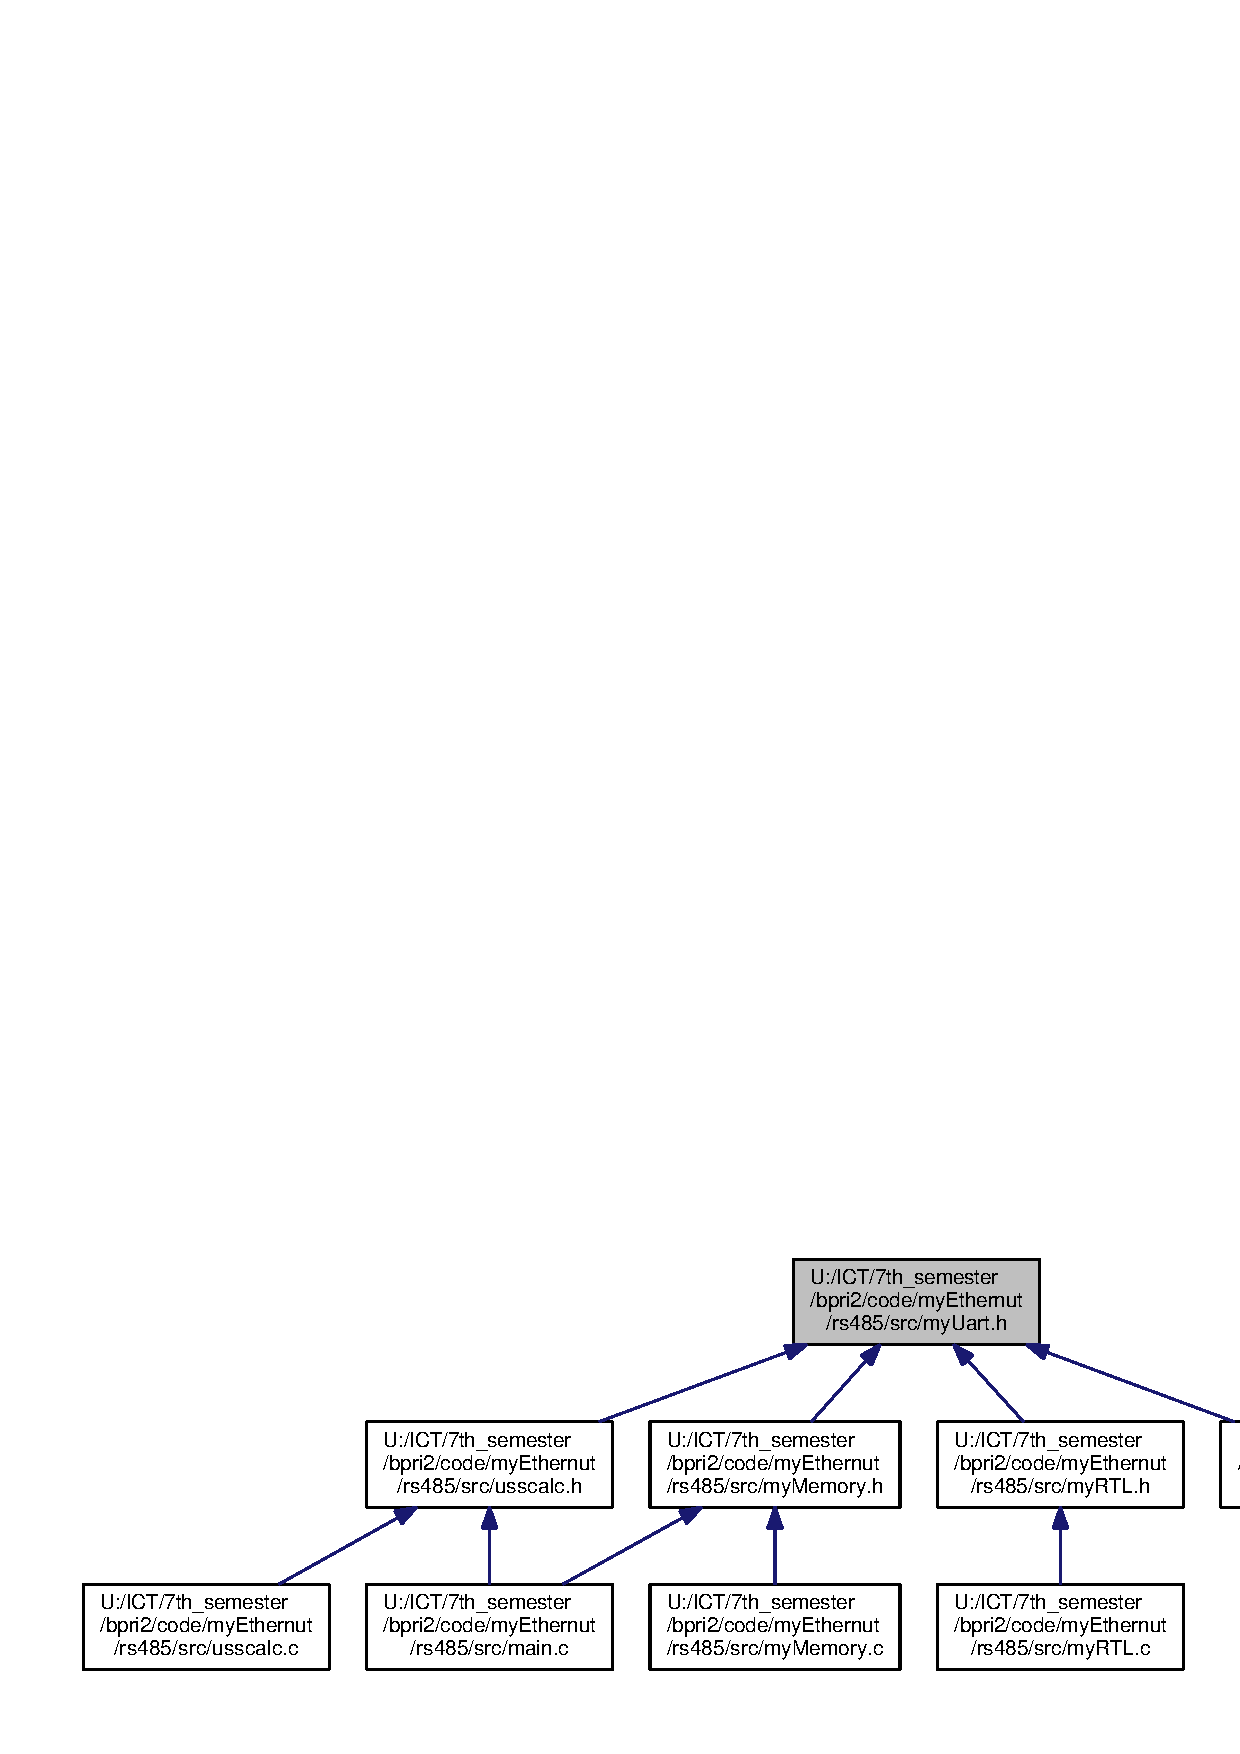
\includegraphics[width=350pt]{my_uart_8h__dep__incl}
\end{center}
\end{figure}
\subsection*{Macros}
\begin{DoxyCompactItemize}
\item 
\#define {\bf F\+\_\+\+C\+P\+U}~14745600\+U\+L
\item 
\#define {\bf B\+A\+U\+D\+R\+A\+T\+E}~115200
\item 
\#define {\bf B\+A\+U\+D\+\_\+\+P\+R\+E\+S\+C\+A\+L\+L\+E\+R}~((({\bf F\+\_\+\+C\+P\+U} / ({\bf B\+A\+U\+D\+R\+A\+T\+E} $\ast$ 16\+U\+L))) -\/ 1)
\end{DoxyCompactItemize}
\subsection*{Functions}
\begin{DoxyCompactItemize}
\item 
void {\bf R\+S232\+\_\+init} (uint32\+\_\+t baudrate)
\item 
void {\bf R\+S485\+\_\+init} (uint32\+\_\+t baudrate)
\item 
unsigned char {\bf R\+S232\+\_\+\+Read\+Char} (void)
\item 
unsigned char {\bf R\+S485\+\_\+\+Read\+Char} (void)
\item 
uint8\+\_\+t $\ast$ {\bf R\+S485\+\_\+\+Query\+Telegram} (uint8\+\_\+t $\ast${\bf my\+Telegram})
\item 
void {\bf R\+S232\+\_\+\+Write\+Char} (unsigned char data)
\item 
void {\bf R\+S485\+\_\+\+Write\+Char} (unsigned char data)
\item 
void {\bf R\+S232\+\_\+putstring} (char $\ast$String\+Ptr)
\item 
void {\bf R\+S485\+\_\+putstring} (char $\ast$String\+Ptr)
\end{DoxyCompactItemize}


\subsection{Macro Definition Documentation}
\index{my\+Uart.\+h@{my\+Uart.\+h}!B\+A\+U\+D\+\_\+\+P\+R\+E\+S\+C\+A\+L\+L\+E\+R@{B\+A\+U\+D\+\_\+\+P\+R\+E\+S\+C\+A\+L\+L\+E\+R}}
\index{B\+A\+U\+D\+\_\+\+P\+R\+E\+S\+C\+A\+L\+L\+E\+R@{B\+A\+U\+D\+\_\+\+P\+R\+E\+S\+C\+A\+L\+L\+E\+R}!my\+Uart.\+h@{my\+Uart.\+h}}
\subsubsection[{B\+A\+U\+D\+\_\+\+P\+R\+E\+S\+C\+A\+L\+L\+E\+R}]{\setlength{\rightskip}{0pt plus 5cm}\#define B\+A\+U\+D\+\_\+\+P\+R\+E\+S\+C\+A\+L\+L\+E\+R~((({\bf F\+\_\+\+C\+P\+U} / ({\bf B\+A\+U\+D\+R\+A\+T\+E} $\ast$ 16\+U\+L))) -\/ 1)}\label{my_uart_8h_a6cbe0c9e92826a80149f453e7788692e}


Definition at line 8 of file my\+Uart.\+h.

\index{my\+Uart.\+h@{my\+Uart.\+h}!B\+A\+U\+D\+R\+A\+T\+E@{B\+A\+U\+D\+R\+A\+T\+E}}
\index{B\+A\+U\+D\+R\+A\+T\+E@{B\+A\+U\+D\+R\+A\+T\+E}!my\+Uart.\+h@{my\+Uart.\+h}}
\subsubsection[{B\+A\+U\+D\+R\+A\+T\+E}]{\setlength{\rightskip}{0pt plus 5cm}\#define B\+A\+U\+D\+R\+A\+T\+E~115200}\label{my_uart_8h_a734bbab06e1a9fd2e5522db0221ff6e3}


Definition at line 7 of file my\+Uart.\+h.

\index{my\+Uart.\+h@{my\+Uart.\+h}!F\+\_\+\+C\+P\+U@{F\+\_\+\+C\+P\+U}}
\index{F\+\_\+\+C\+P\+U@{F\+\_\+\+C\+P\+U}!my\+Uart.\+h@{my\+Uart.\+h}}
\subsubsection[{F\+\_\+\+C\+P\+U}]{\setlength{\rightskip}{0pt plus 5cm}\#define F\+\_\+\+C\+P\+U~14745600\+U\+L}\label{my_uart_8h_a43bafb28b29491ec7f871319b5a3b2f8}


Definition at line 6 of file my\+Uart.\+h.



Referenced by R\+S232\+\_\+init(), and R\+S485\+\_\+init().



\subsection{Function Documentation}
\index{my\+Uart.\+h@{my\+Uart.\+h}!R\+S232\+\_\+init@{R\+S232\+\_\+init}}
\index{R\+S232\+\_\+init@{R\+S232\+\_\+init}!my\+Uart.\+h@{my\+Uart.\+h}}
\subsubsection[{R\+S232\+\_\+init(uint32\+\_\+t baudrate)}]{\setlength{\rightskip}{0pt plus 5cm}void R\+S232\+\_\+init (
\begin{DoxyParamCaption}
\item[{uint32\+\_\+t}]{baudrate}
\end{DoxyParamCaption}
)}\label{my_uart_8h_a06c2a1060a933565013c7e5977139244}


Definition at line 92 of file my\+Uart.\+c.



References F\+\_\+\+C\+P\+U.



Referenced by main().

\index{my\+Uart.\+h@{my\+Uart.\+h}!R\+S232\+\_\+putstring@{R\+S232\+\_\+putstring}}
\index{R\+S232\+\_\+putstring@{R\+S232\+\_\+putstring}!my\+Uart.\+h@{my\+Uart.\+h}}
\subsubsection[{R\+S232\+\_\+putstring(char $\ast$\+String\+Ptr)}]{\setlength{\rightskip}{0pt plus 5cm}void R\+S232\+\_\+putstring (
\begin{DoxyParamCaption}
\item[{char $\ast$}]{String\+Ptr}
\end{DoxyParamCaption}
)}\label{my_uart_8h_a60eaeaa21312415e8b5c05f5376f3541}


Definition at line 77 of file my\+Uart.\+c.



References R\+S232\+\_\+\+Write\+Char().



Referenced by deb\+\_\+print(), display\+Telegram(), main(), print\+\_\+bin\+Byte(), print\+\_\+hex\+Address(), print\+\_\+hex\+Byte(), print\+\_\+hex\+Word(), read\+R\+T\+L\+Memory(), Test\+External\+Ram(), test\+Memory(), and Test\+Realtek().



Here is the call graph for this function\+:\nopagebreak
\begin{figure}[H]
\begin{center}
\leavevmode
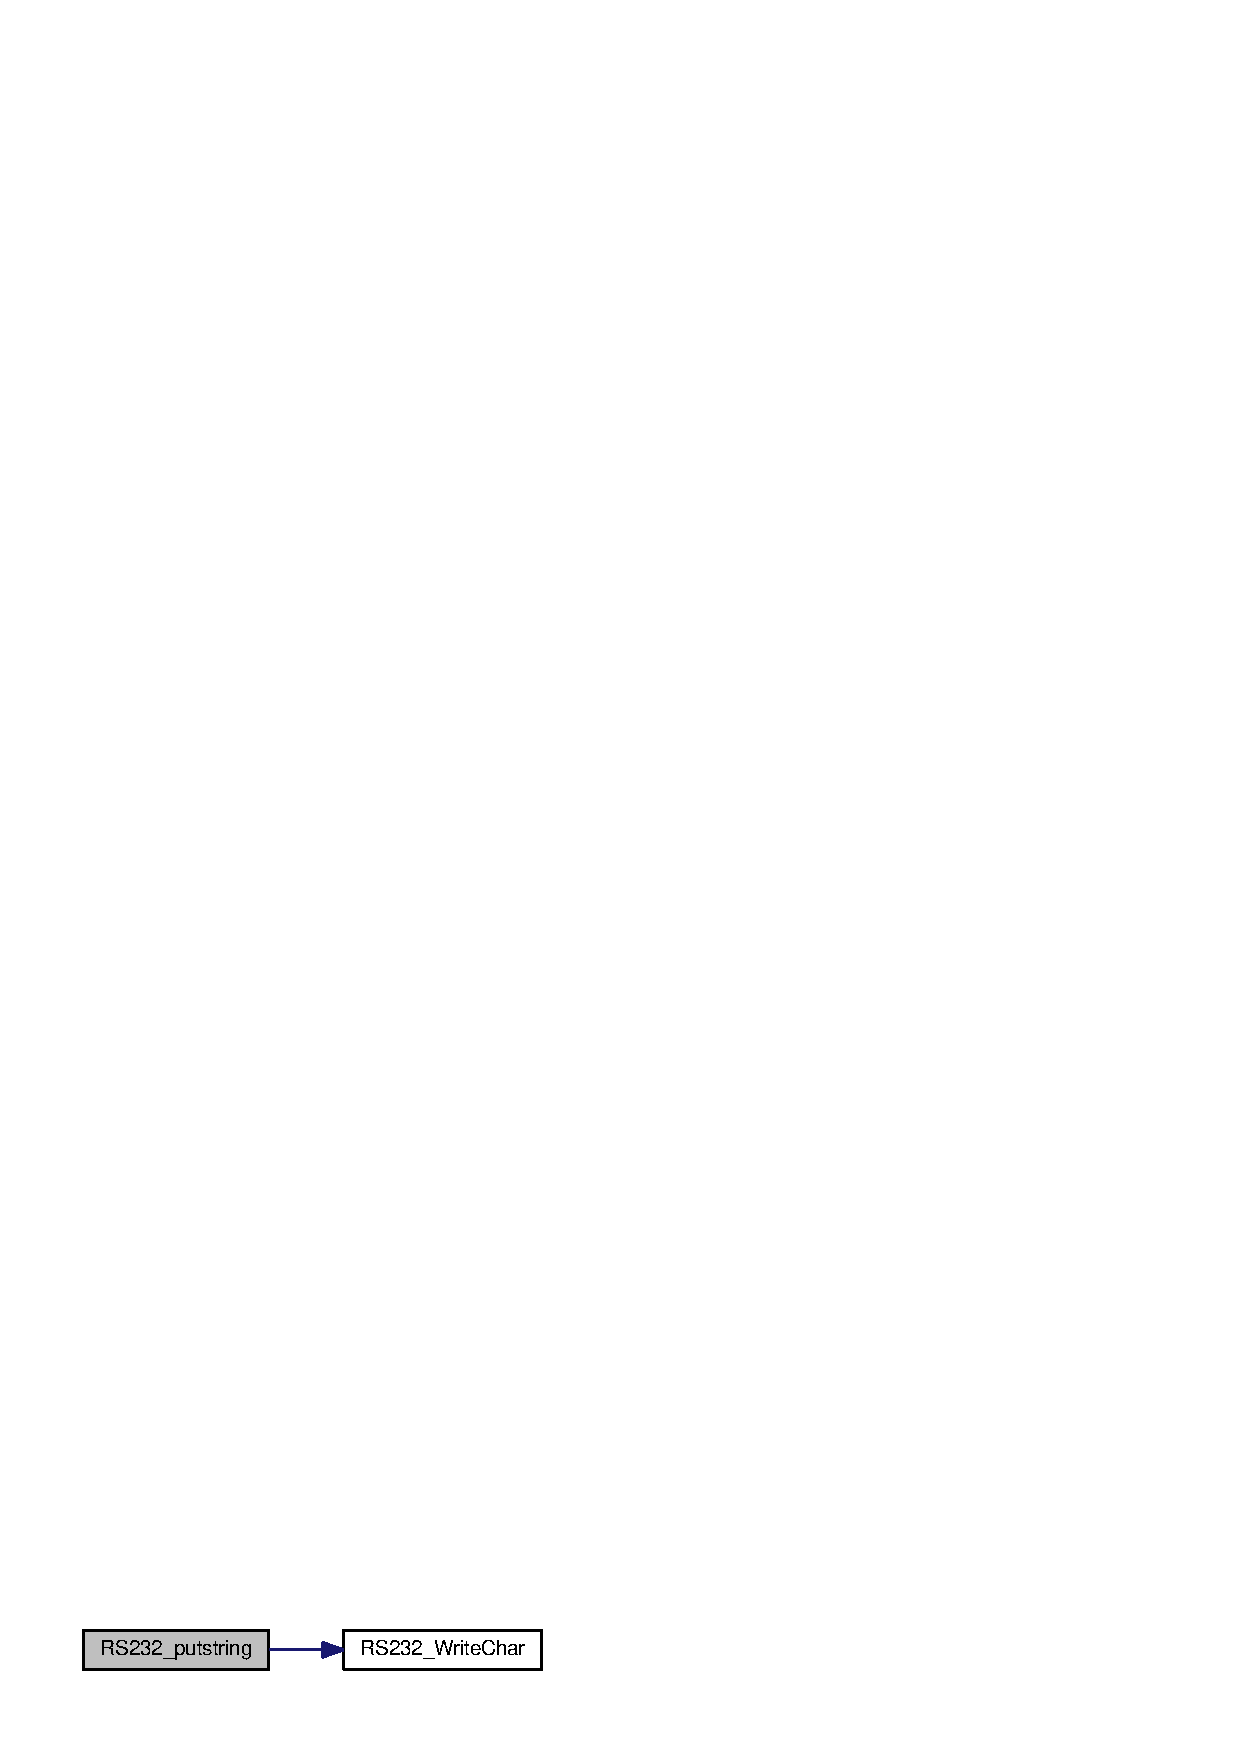
\includegraphics[width=264pt]{my_uart_8h_a60eaeaa21312415e8b5c05f5376f3541_cgraph}
\end{center}
\end{figure}


\index{my\+Uart.\+h@{my\+Uart.\+h}!R\+S232\+\_\+\+Read\+Char@{R\+S232\+\_\+\+Read\+Char}}
\index{R\+S232\+\_\+\+Read\+Char@{R\+S232\+\_\+\+Read\+Char}!my\+Uart.\+h@{my\+Uart.\+h}}
\subsubsection[{R\+S232\+\_\+\+Read\+Char(void)}]{\setlength{\rightskip}{0pt plus 5cm}unsigned char R\+S232\+\_\+\+Read\+Char (
\begin{DoxyParamCaption}
\item[{void}]{}
\end{DoxyParamCaption}
)}\label{my_uart_8h_a50356f8980826894751733073e37ec41}


Definition at line 6 of file my\+Uart.\+c.

\index{my\+Uart.\+h@{my\+Uart.\+h}!R\+S232\+\_\+\+Write\+Char@{R\+S232\+\_\+\+Write\+Char}}
\index{R\+S232\+\_\+\+Write\+Char@{R\+S232\+\_\+\+Write\+Char}!my\+Uart.\+h@{my\+Uart.\+h}}
\subsubsection[{R\+S232\+\_\+\+Write\+Char(unsigned char data)}]{\setlength{\rightskip}{0pt plus 5cm}void R\+S232\+\_\+\+Write\+Char (
\begin{DoxyParamCaption}
\item[{unsigned char}]{data}
\end{DoxyParamCaption}
)}\label{my_uart_8h_a1a99be79a25c05250ff2eca4cbbf9fc5}


Definition at line 24 of file my\+Uart.\+c.



Referenced by print\+\_\+bin\+Byte(), and R\+S232\+\_\+putstring().

\index{my\+Uart.\+h@{my\+Uart.\+h}!R\+S485\+\_\+init@{R\+S485\+\_\+init}}
\index{R\+S485\+\_\+init@{R\+S485\+\_\+init}!my\+Uart.\+h@{my\+Uart.\+h}}
\subsubsection[{R\+S485\+\_\+init(uint32\+\_\+t baudrate)}]{\setlength{\rightskip}{0pt plus 5cm}void R\+S485\+\_\+init (
\begin{DoxyParamCaption}
\item[{uint32\+\_\+t}]{baudrate}
\end{DoxyParamCaption}
)}\label{my_uart_8h_a27f5340823874f42a318aab1e8b4ed50}


Definition at line 103 of file my\+Uart.\+c.



References F\+\_\+\+C\+P\+U.



Referenced by main().

\index{my\+Uart.\+h@{my\+Uart.\+h}!R\+S485\+\_\+putstring@{R\+S485\+\_\+putstring}}
\index{R\+S485\+\_\+putstring@{R\+S485\+\_\+putstring}!my\+Uart.\+h@{my\+Uart.\+h}}
\subsubsection[{R\+S485\+\_\+putstring(char $\ast$\+String\+Ptr)}]{\setlength{\rightskip}{0pt plus 5cm}void R\+S485\+\_\+putstring (
\begin{DoxyParamCaption}
\item[{char $\ast$}]{String\+Ptr}
\end{DoxyParamCaption}
)}\label{my_uart_8h_accde78cd49a35a1dbb5100640334492b}


Definition at line 84 of file my\+Uart.\+c.



References R\+S485\+\_\+\+Write\+Char().



Here is the call graph for this function\+:\nopagebreak
\begin{figure}[H]
\begin{center}
\leavevmode
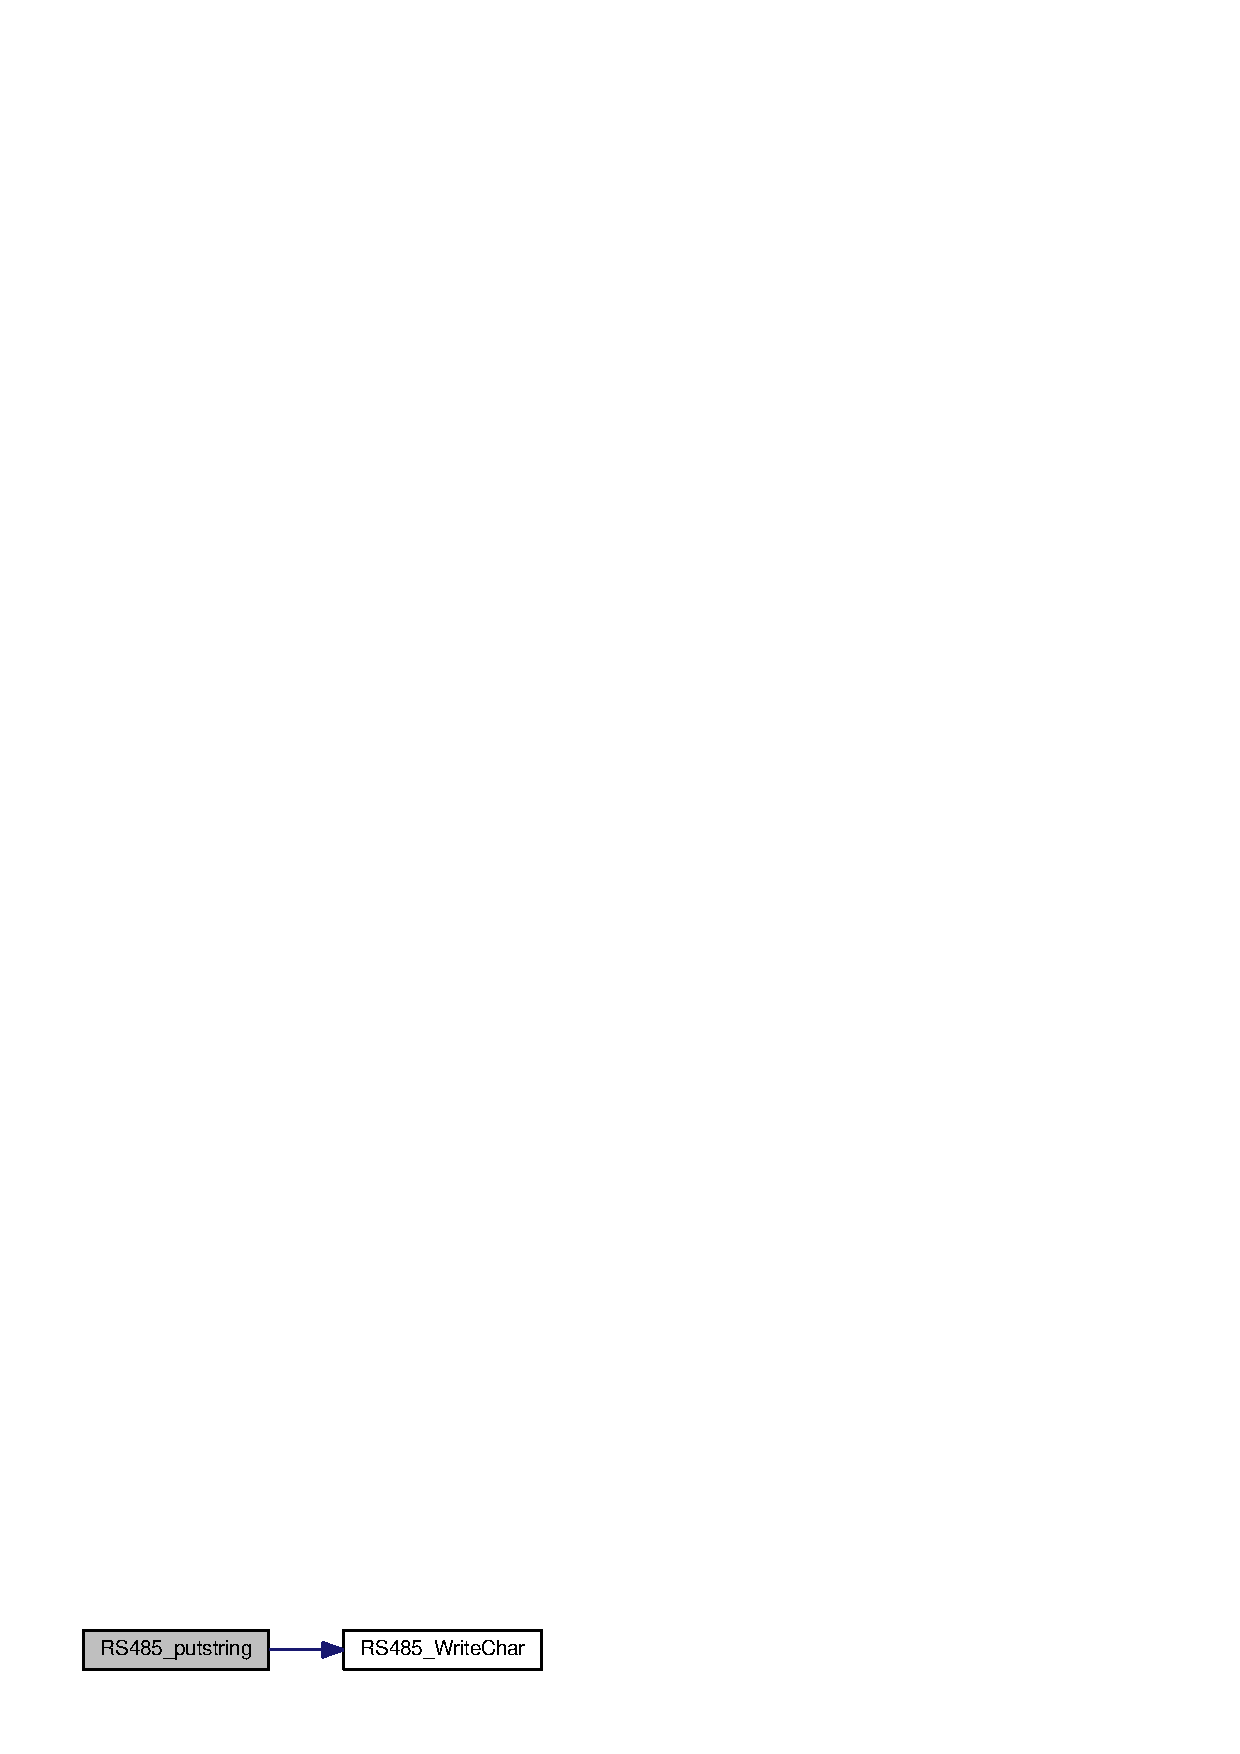
\includegraphics[width=264pt]{my_uart_8h_accde78cd49a35a1dbb5100640334492b_cgraph}
\end{center}
\end{figure}


\index{my\+Uart.\+h@{my\+Uart.\+h}!R\+S485\+\_\+\+Query\+Telegram@{R\+S485\+\_\+\+Query\+Telegram}}
\index{R\+S485\+\_\+\+Query\+Telegram@{R\+S485\+\_\+\+Query\+Telegram}!my\+Uart.\+h@{my\+Uart.\+h}}
\subsubsection[{R\+S485\+\_\+\+Query\+Telegram(uint8\+\_\+t $\ast$my\+Telegram)}]{\setlength{\rightskip}{0pt plus 5cm}uint8\+\_\+t$\ast$ R\+S485\+\_\+\+Query\+Telegram (
\begin{DoxyParamCaption}
\item[{uint8\+\_\+t $\ast$}]{my\+Telegram}
\end{DoxyParamCaption}
)}\label{my_uart_8h_a9b1299202b28a668b8039f538539efb1}


Definition at line 52 of file my\+Uart.\+c.



References my\+Telegram, R\+S485\+\_\+\+Read\+Char(), and R\+S485\+\_\+\+Write\+Char().



Referenced by get\+Value().



Here is the call graph for this function\+:\nopagebreak
\begin{figure}[H]
\begin{center}
\leavevmode
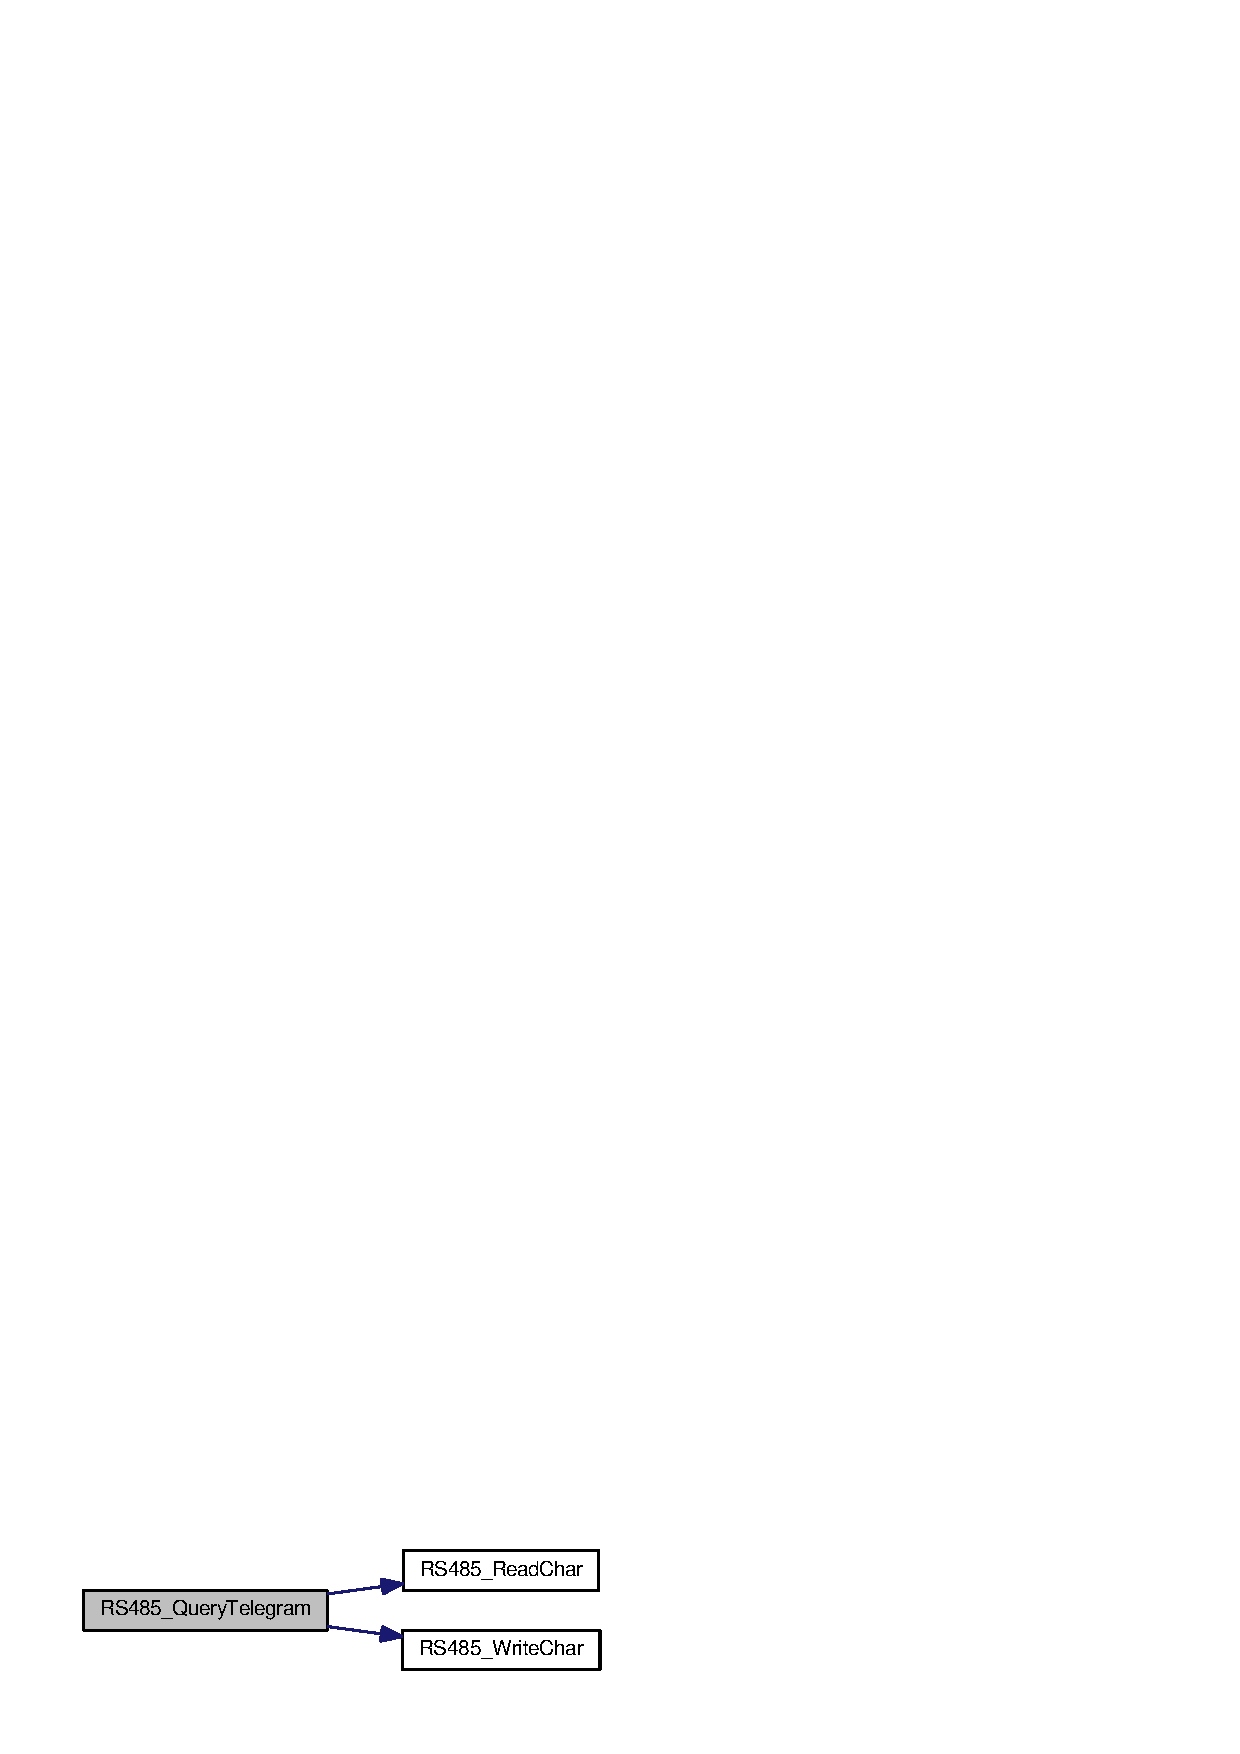
\includegraphics[width=292pt]{my_uart_8h_a9b1299202b28a668b8039f538539efb1_cgraph}
\end{center}
\end{figure}


\index{my\+Uart.\+h@{my\+Uart.\+h}!R\+S485\+\_\+\+Read\+Char@{R\+S485\+\_\+\+Read\+Char}}
\index{R\+S485\+\_\+\+Read\+Char@{R\+S485\+\_\+\+Read\+Char}!my\+Uart.\+h@{my\+Uart.\+h}}
\subsubsection[{R\+S485\+\_\+\+Read\+Char(void)}]{\setlength{\rightskip}{0pt plus 5cm}unsigned char R\+S485\+\_\+\+Read\+Char (
\begin{DoxyParamCaption}
\item[{void}]{}
\end{DoxyParamCaption}
)}\label{my_uart_8h_ab56f53b4e7d6fe7165cdef32270c7a39}


Definition at line 14 of file my\+Uart.\+c.



Referenced by R\+S485\+\_\+\+Query\+Telegram().

\index{my\+Uart.\+h@{my\+Uart.\+h}!R\+S485\+\_\+\+Write\+Char@{R\+S485\+\_\+\+Write\+Char}}
\index{R\+S485\+\_\+\+Write\+Char@{R\+S485\+\_\+\+Write\+Char}!my\+Uart.\+h@{my\+Uart.\+h}}
\subsubsection[{R\+S485\+\_\+\+Write\+Char(unsigned char data)}]{\setlength{\rightskip}{0pt plus 5cm}void R\+S485\+\_\+\+Write\+Char (
\begin{DoxyParamCaption}
\item[{unsigned char}]{data}
\end{DoxyParamCaption}
)}\label{my_uart_8h_aeb49100d16c0c1b323128896ed286558}


Definition at line 32 of file my\+Uart.\+c.



Referenced by R\+S485\+\_\+putstring(), and R\+S485\+\_\+\+Query\+Telegram().


\section{U\+:/\+I\+C\+T/7th\+\_\+semester/bpri2/code/my\+Ethernut/rs485/src/my\+Util.c File Reference}
\label{my_util_8c}\index{U\+:/\+I\+C\+T/7th\+\_\+semester/bpri2/code/my\+Ethernut/rs485/src/my\+Util.\+c@{U\+:/\+I\+C\+T/7th\+\_\+semester/bpri2/code/my\+Ethernut/rs485/src/my\+Util.\+c}}
{\ttfamily \#include \char`\"{}my\+Util.\+h\char`\"{}}\\*
Include dependency graph for my\+Util.\+c\+:\nopagebreak
\begin{figure}[H]
\begin{center}
\leavevmode
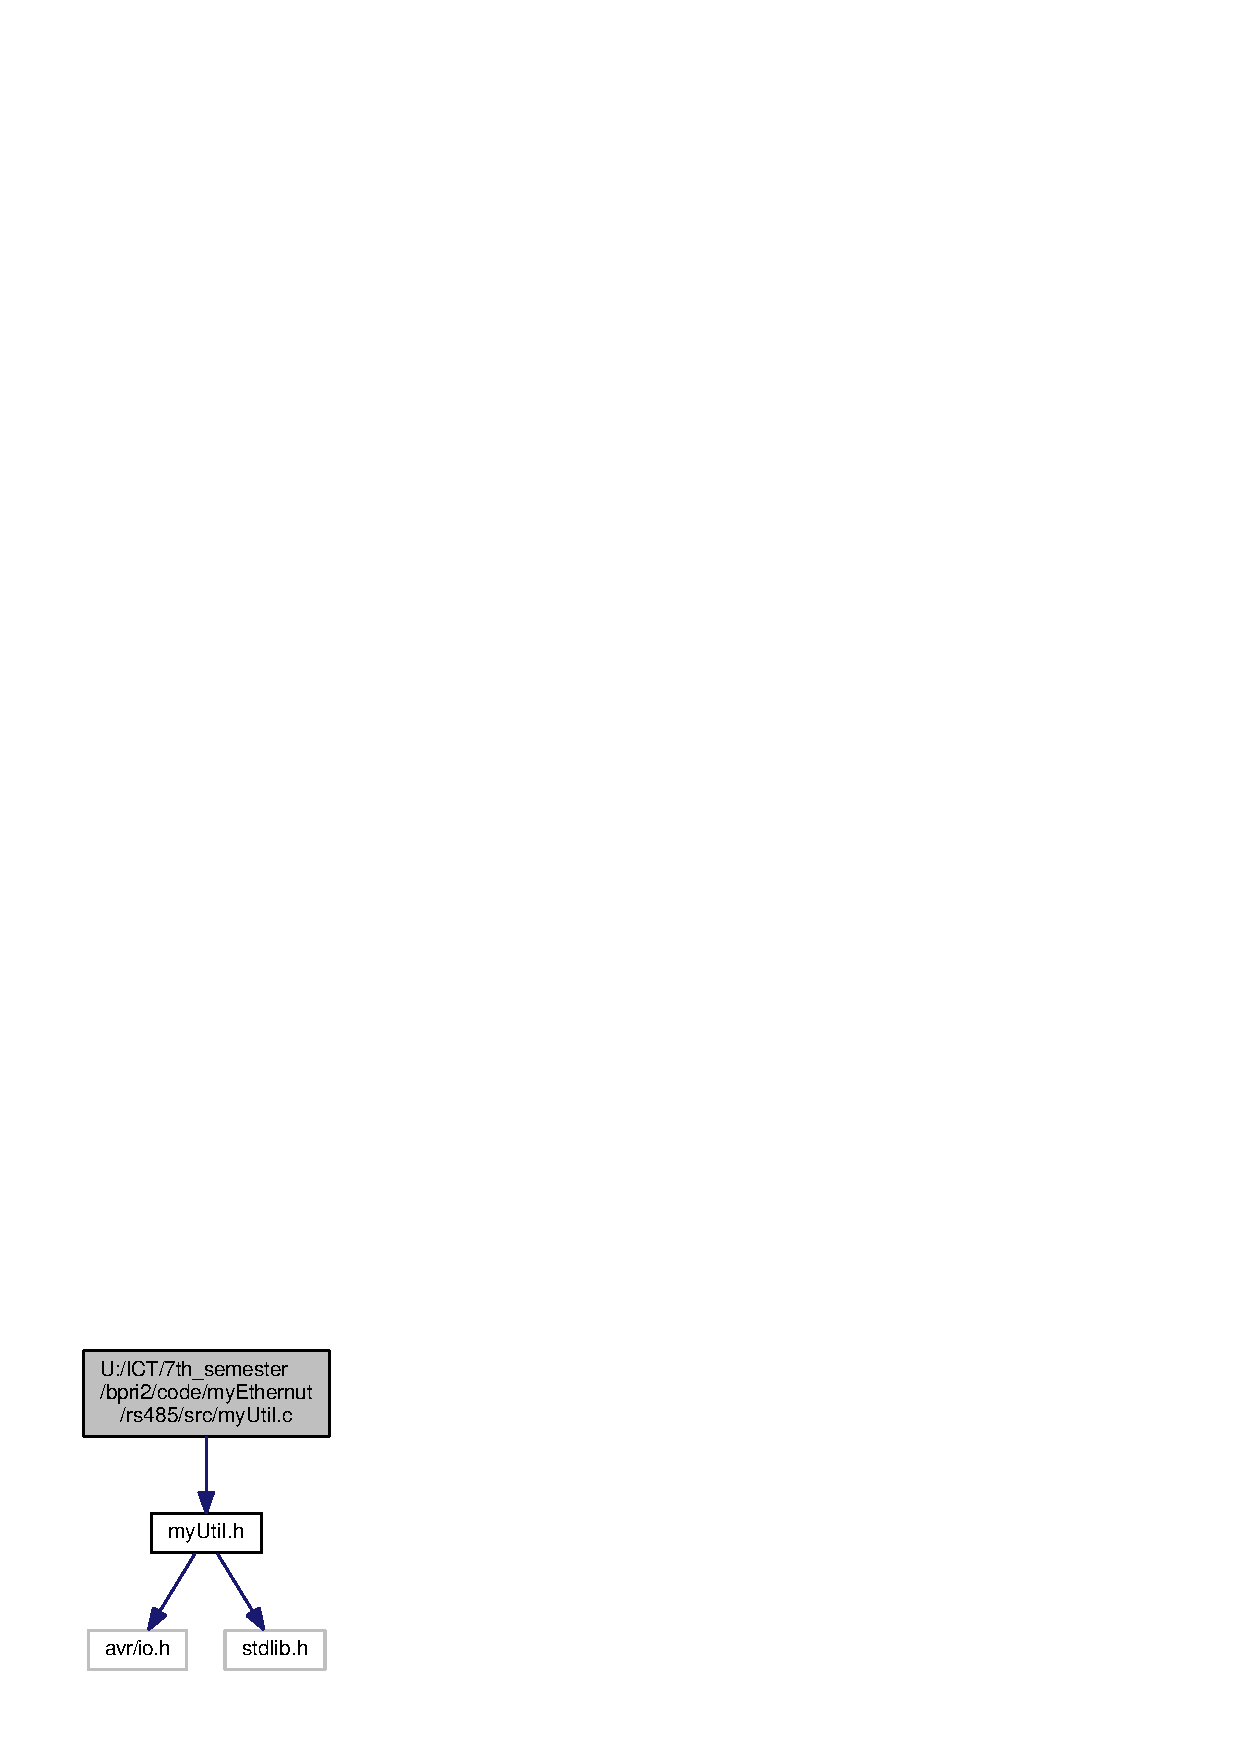
\includegraphics[width=162pt]{my_util_8c__incl}
\end{center}
\end{figure}
\subsection*{Functions}
\begin{DoxyCompactItemize}
\item 
void {\bf print\+\_\+bin\+Byte} (uint8\+\_\+t my\+Byte)
\item 
void {\bf print\+\_\+hex\+Byte} (uint8\+\_\+t my\+Byte)
\item 
void {\bf print\+\_\+hex\+Word} (uint16\+\_\+t hword)
\item 
void {\bf print\+\_\+hex\+Address} (uint16\+\_\+t address)
\item 
void {\bf print\+Str\+In\+Hex} (char $\ast$a\+String)
\item 
void {\bf deb\+\_\+print} (char $\ast$a\+String, uint8\+\_\+t byte)
\end{DoxyCompactItemize}


\subsection{Function Documentation}
\index{my\+Util.\+c@{my\+Util.\+c}!deb\+\_\+print@{deb\+\_\+print}}
\index{deb\+\_\+print@{deb\+\_\+print}!my\+Util.\+c@{my\+Util.\+c}}
\subsubsection[{deb\+\_\+print(char $\ast$a\+String, uint8\+\_\+t byte)}]{\setlength{\rightskip}{0pt plus 5cm}void deb\+\_\+print (
\begin{DoxyParamCaption}
\item[{char $\ast$}]{a\+String, }
\item[{uint8\+\_\+t}]{byte}
\end{DoxyParamCaption}
)}\label{my_util_8c_a2f9f5b067182da7e5194b95dd69796d5}


Definition at line 179 of file my\+Util.\+c.



References R\+S232\+\_\+putstring().



Here is the call graph for this function\+:\nopagebreak
\begin{figure}[H]
\begin{center}
\leavevmode
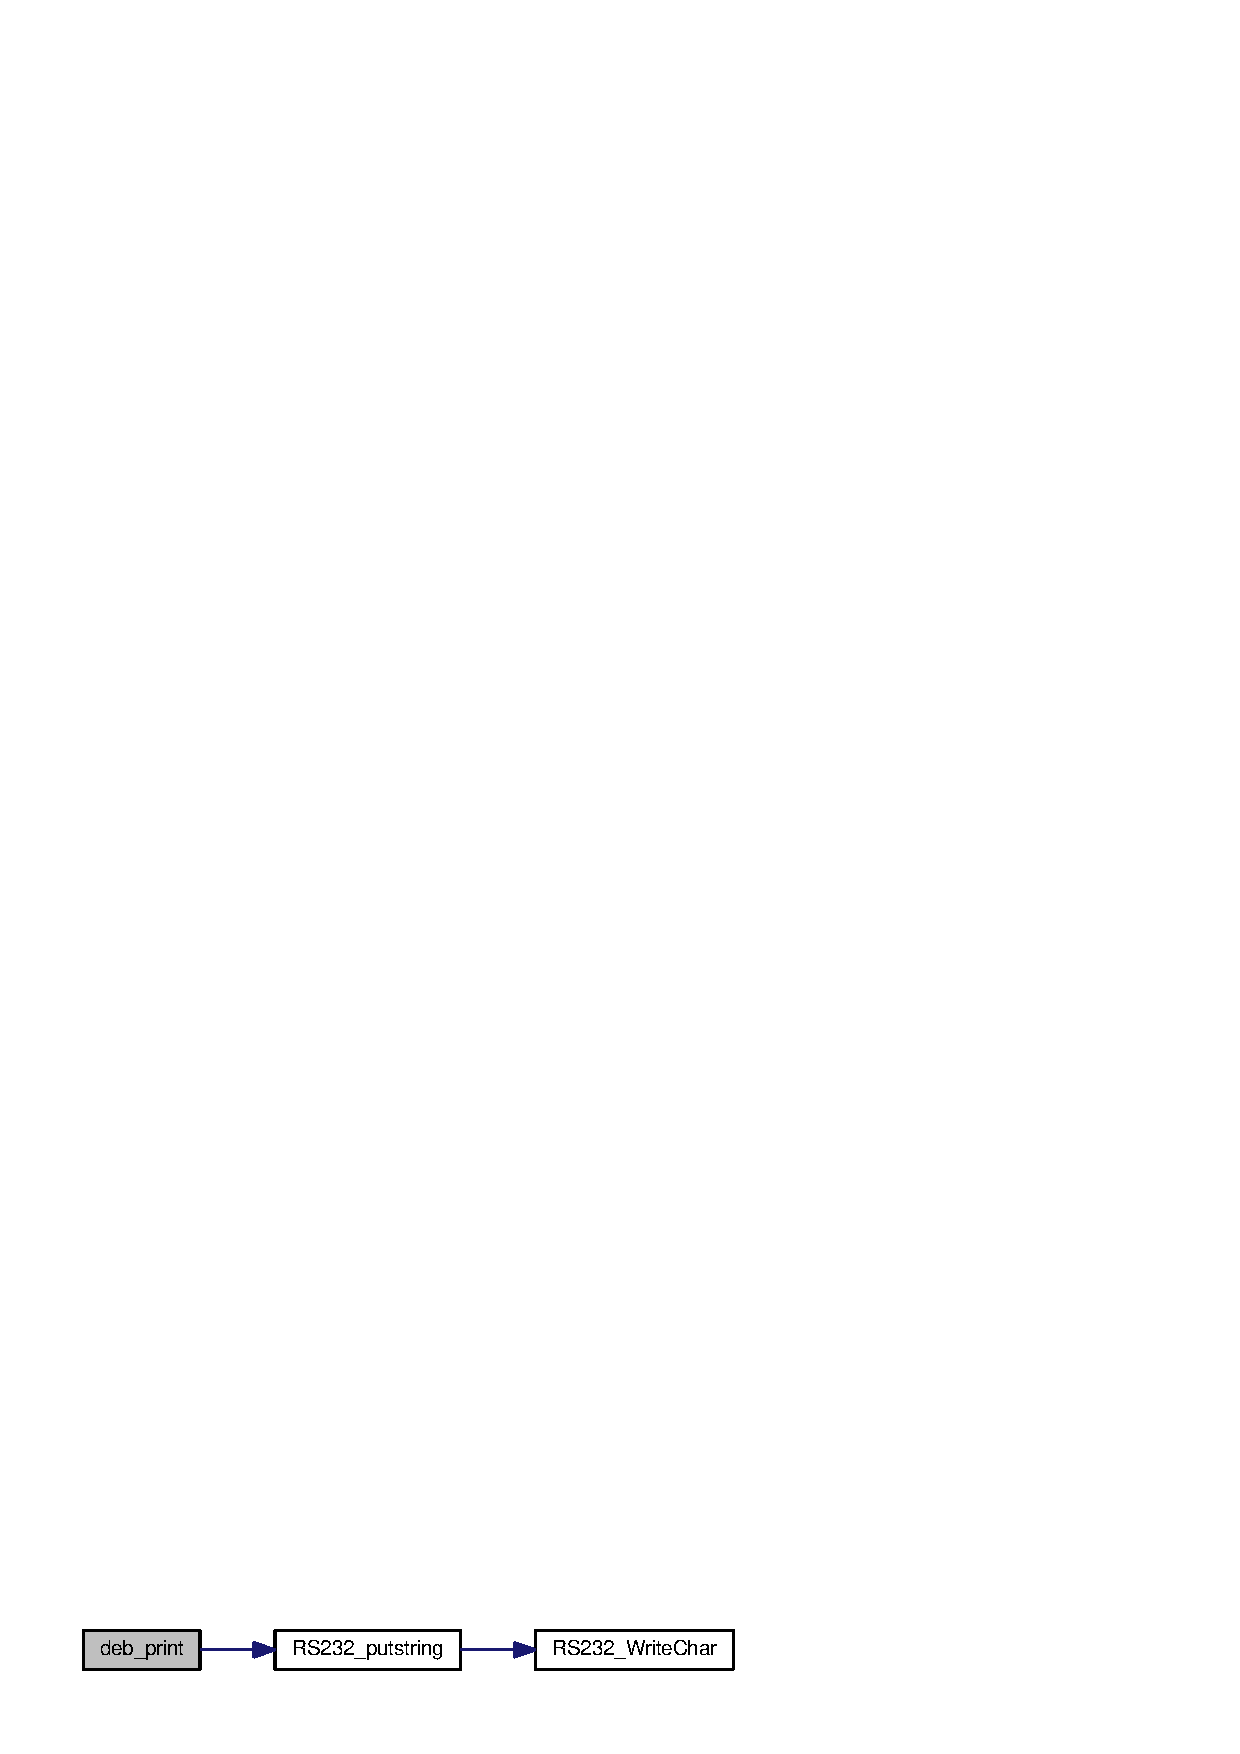
\includegraphics[width=350pt]{my_util_8c_a2f9f5b067182da7e5194b95dd69796d5_cgraph}
\end{center}
\end{figure}


\index{my\+Util.\+c@{my\+Util.\+c}!print\+\_\+bin\+Byte@{print\+\_\+bin\+Byte}}
\index{print\+\_\+bin\+Byte@{print\+\_\+bin\+Byte}!my\+Util.\+c@{my\+Util.\+c}}
\subsubsection[{print\+\_\+bin\+Byte(uint8\+\_\+t my\+Byte)}]{\setlength{\rightskip}{0pt plus 5cm}void print\+\_\+bin\+Byte (
\begin{DoxyParamCaption}
\item[{uint8\+\_\+t}]{my\+Byte}
\end{DoxyParamCaption}
)}\label{my_util_8c_a446d5fa92eead663eb3c401c3728b49f}


Definition at line 16 of file my\+Util.\+c.



References R\+S232\+\_\+putstring(), and R\+S232\+\_\+\+Write\+Char().



Here is the call graph for this function\+:\nopagebreak
\begin{figure}[H]
\begin{center}
\leavevmode
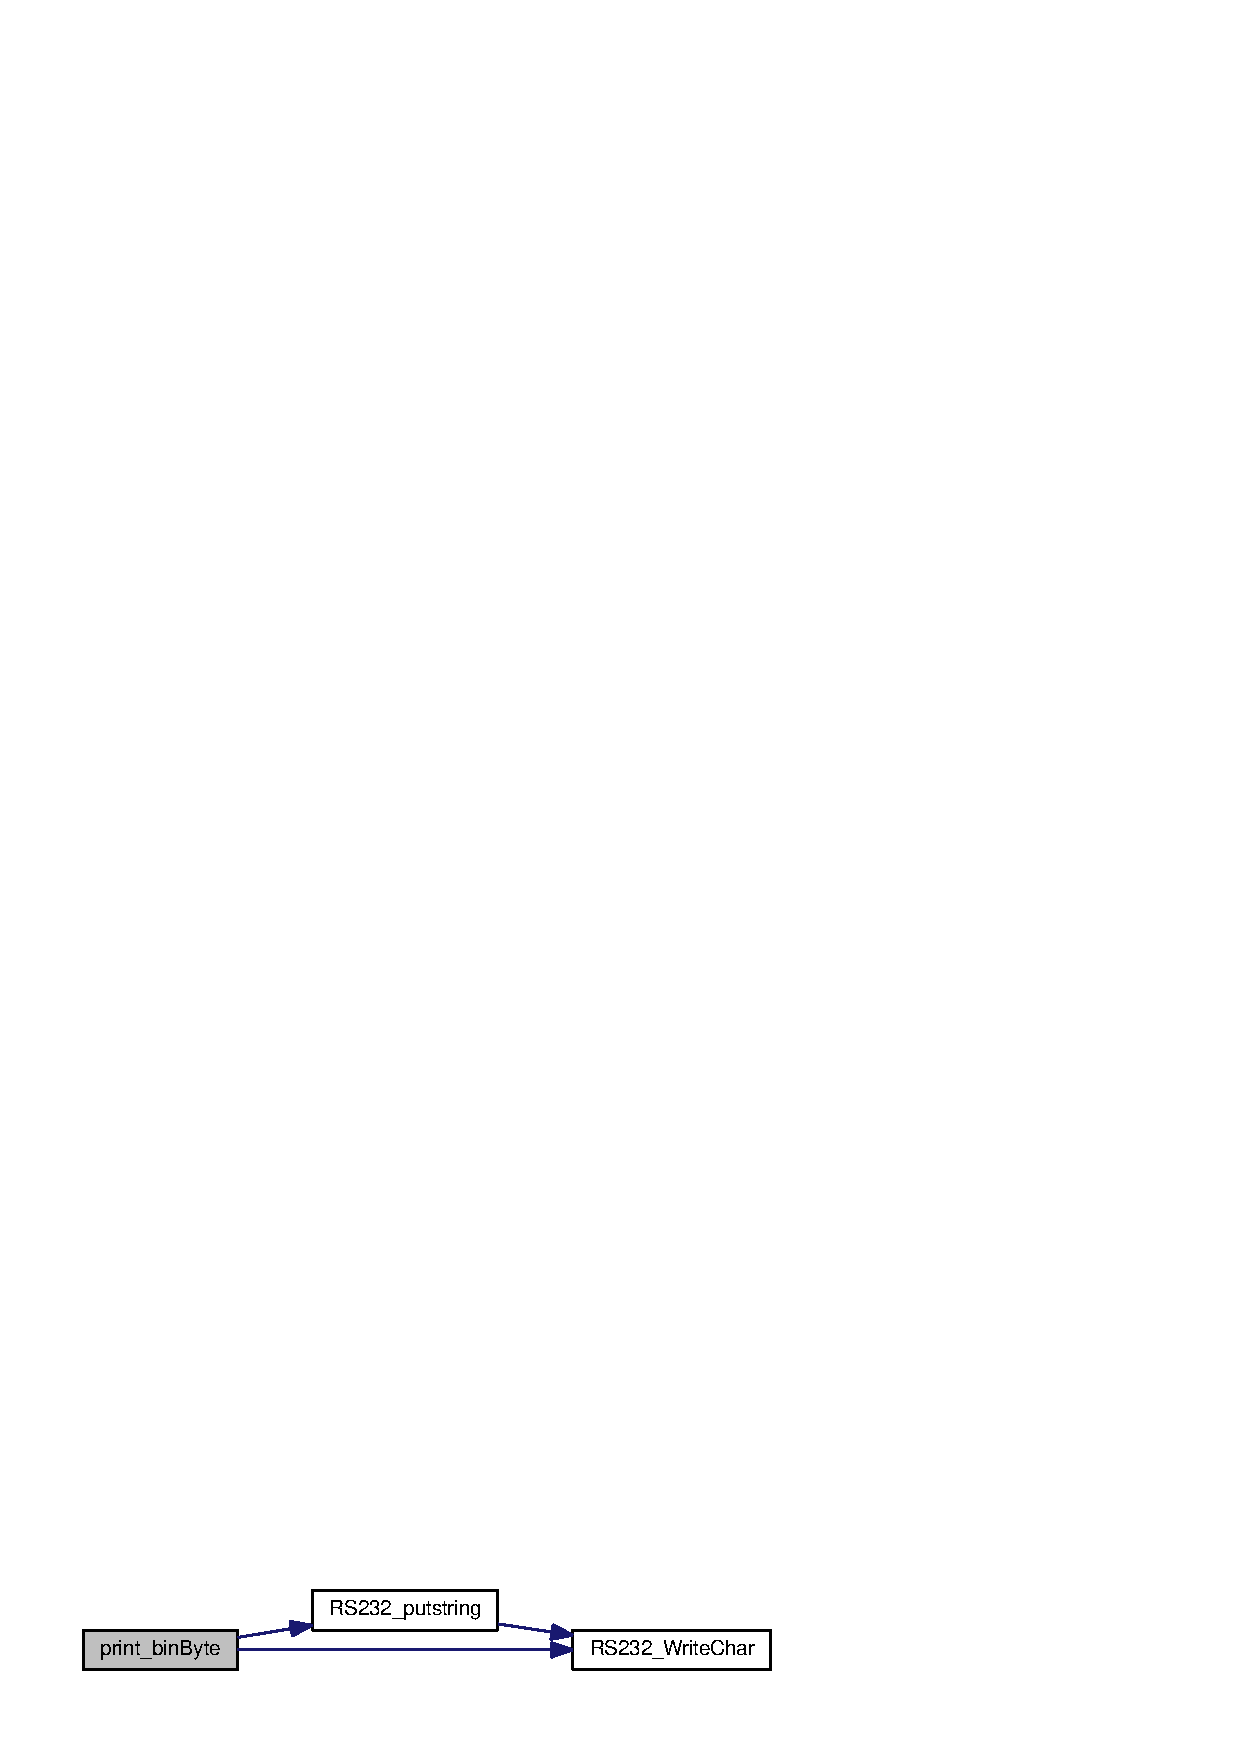
\includegraphics[width=350pt]{my_util_8c_a446d5fa92eead663eb3c401c3728b49f_cgraph}
\end{center}
\end{figure}


\index{my\+Util.\+c@{my\+Util.\+c}!print\+\_\+hex\+Address@{print\+\_\+hex\+Address}}
\index{print\+\_\+hex\+Address@{print\+\_\+hex\+Address}!my\+Util.\+c@{my\+Util.\+c}}
\subsubsection[{print\+\_\+hex\+Address(uint16\+\_\+t address)}]{\setlength{\rightskip}{0pt plus 5cm}void print\+\_\+hex\+Address (
\begin{DoxyParamCaption}
\item[{uint16\+\_\+t}]{address}
\end{DoxyParamCaption}
)}\label{my_util_8c_afb61822546c6e61b88e5e165764a3ccb}


Definition at line 109 of file my\+Util.\+c.



References R\+S232\+\_\+putstring().



Referenced by read\+R\+T\+L\+Memory(), and test\+Memory().



Here is the call graph for this function\+:\nopagebreak
\begin{figure}[H]
\begin{center}
\leavevmode
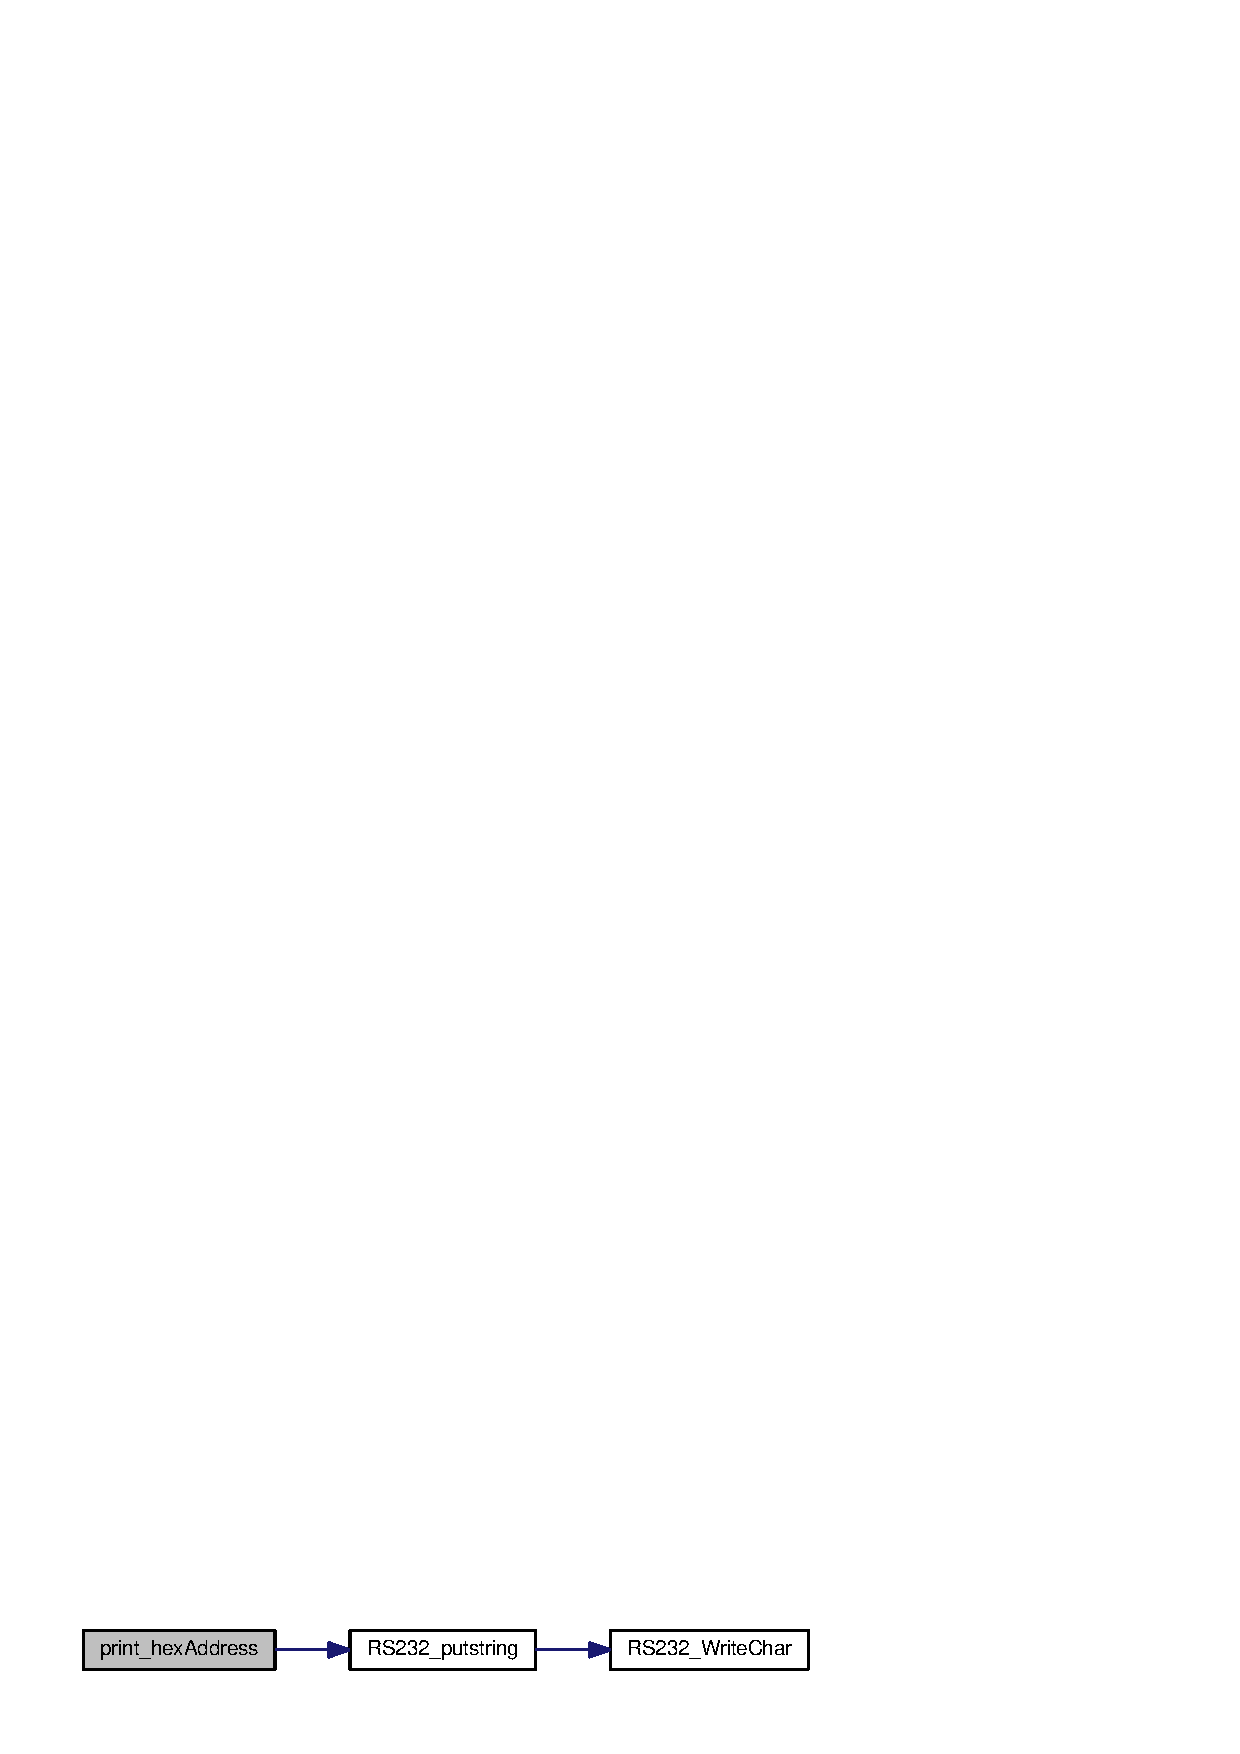
\includegraphics[width=350pt]{my_util_8c_afb61822546c6e61b88e5e165764a3ccb_cgraph}
\end{center}
\end{figure}


\index{my\+Util.\+c@{my\+Util.\+c}!print\+\_\+hex\+Byte@{print\+\_\+hex\+Byte}}
\index{print\+\_\+hex\+Byte@{print\+\_\+hex\+Byte}!my\+Util.\+c@{my\+Util.\+c}}
\subsubsection[{print\+\_\+hex\+Byte(uint8\+\_\+t my\+Byte)}]{\setlength{\rightskip}{0pt plus 5cm}void print\+\_\+hex\+Byte (
\begin{DoxyParamCaption}
\item[{uint8\+\_\+t}]{my\+Byte}
\end{DoxyParamCaption}
)}\label{my_util_8c_aebd073f6dad448b0012eef8a8fd982fb}


Definition at line 35 of file my\+Util.\+c.



References R\+S232\+\_\+putstring().



Referenced by display\+Telegram(), print\+Str\+In\+Hex(), and Test\+External\+Ram().



Here is the call graph for this function\+:\nopagebreak
\begin{figure}[H]
\begin{center}
\leavevmode
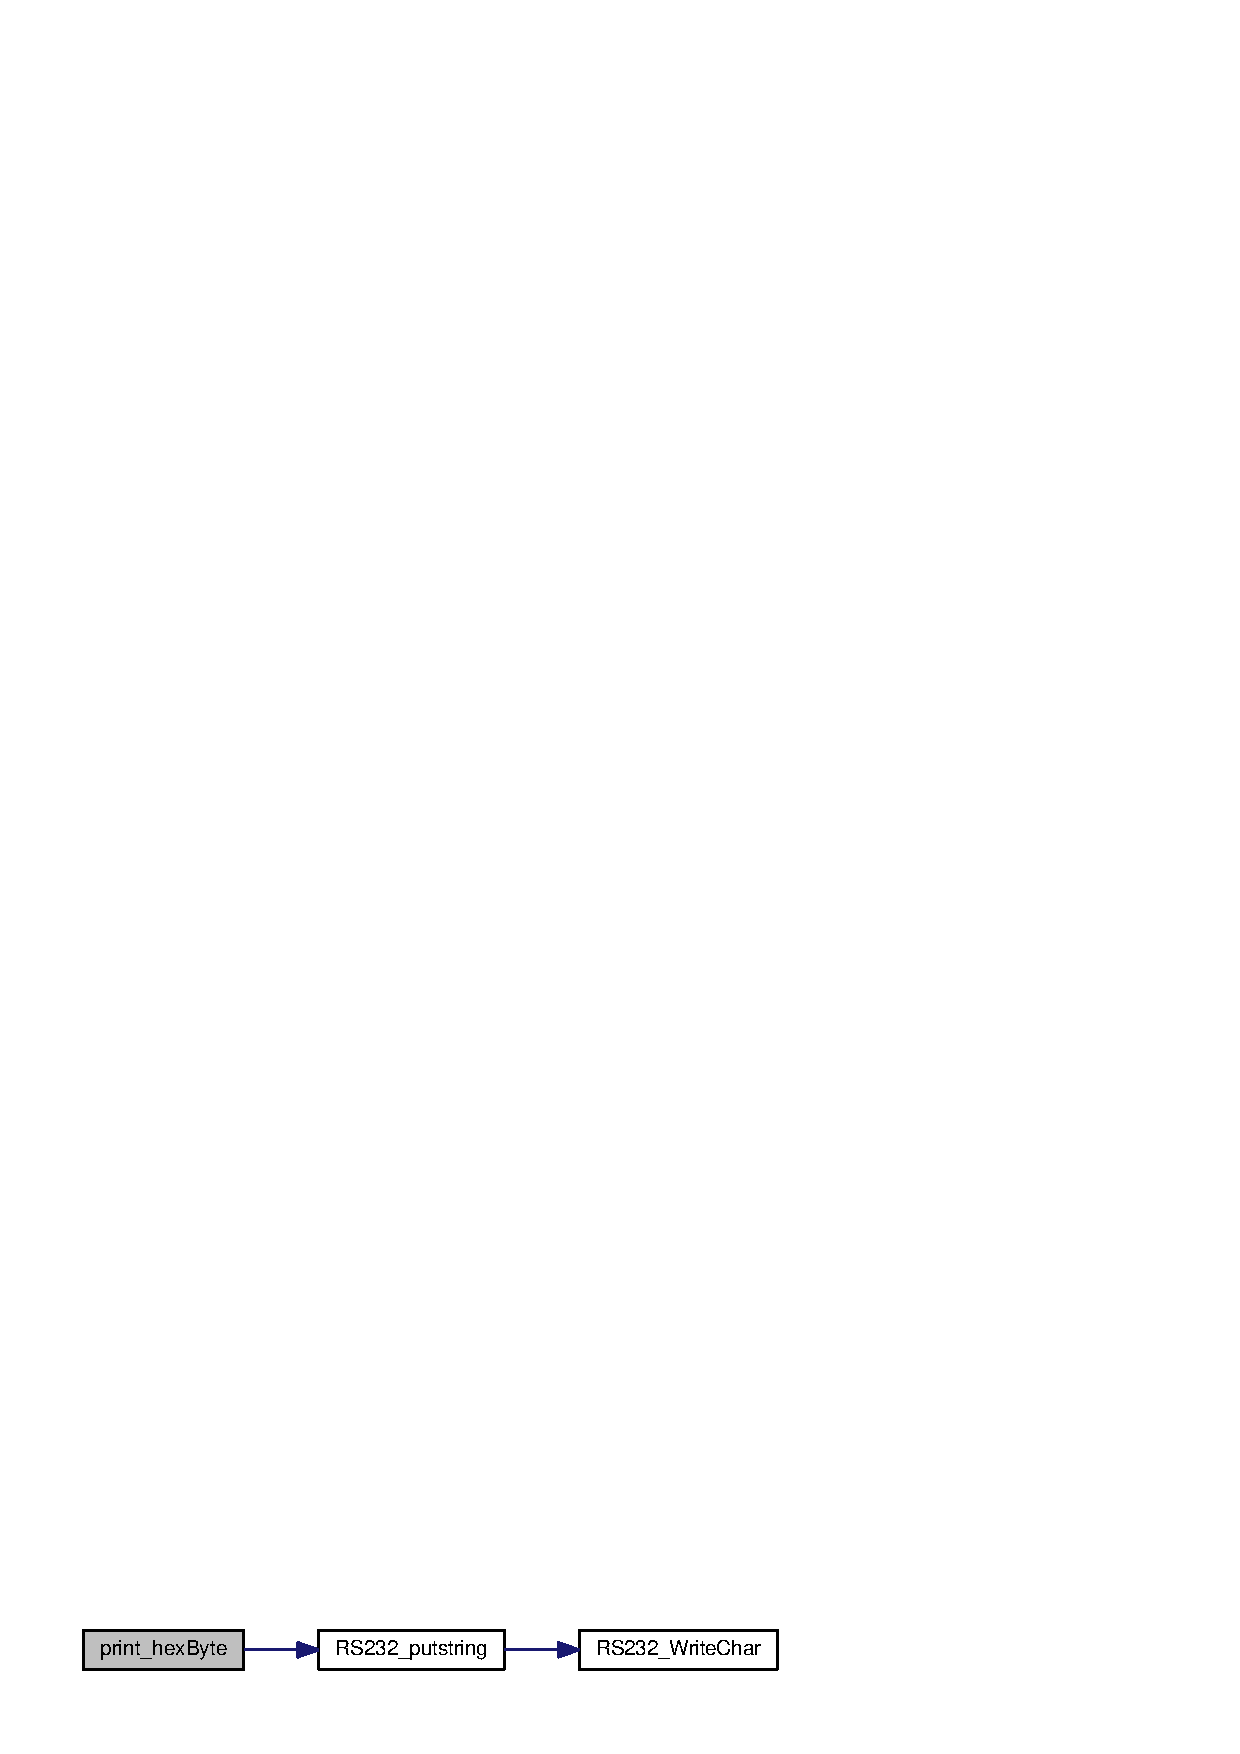
\includegraphics[width=350pt]{my_util_8c_aebd073f6dad448b0012eef8a8fd982fb_cgraph}
\end{center}
\end{figure}


\index{my\+Util.\+c@{my\+Util.\+c}!print\+\_\+hex\+Word@{print\+\_\+hex\+Word}}
\index{print\+\_\+hex\+Word@{print\+\_\+hex\+Word}!my\+Util.\+c@{my\+Util.\+c}}
\subsubsection[{print\+\_\+hex\+Word(uint16\+\_\+t hword)}]{\setlength{\rightskip}{0pt plus 5cm}void print\+\_\+hex\+Word (
\begin{DoxyParamCaption}
\item[{uint16\+\_\+t}]{hword}
\end{DoxyParamCaption}
)}\label{my_util_8c_a462f788430a8411cca8cfe2116118e31}


Definition at line 49 of file my\+Util.\+c.



References R\+S232\+\_\+putstring().



Referenced by main(), read\+R\+T\+L\+Memory(), test\+Memory(), and Test\+Realtek().



Here is the call graph for this function\+:\nopagebreak
\begin{figure}[H]
\begin{center}
\leavevmode
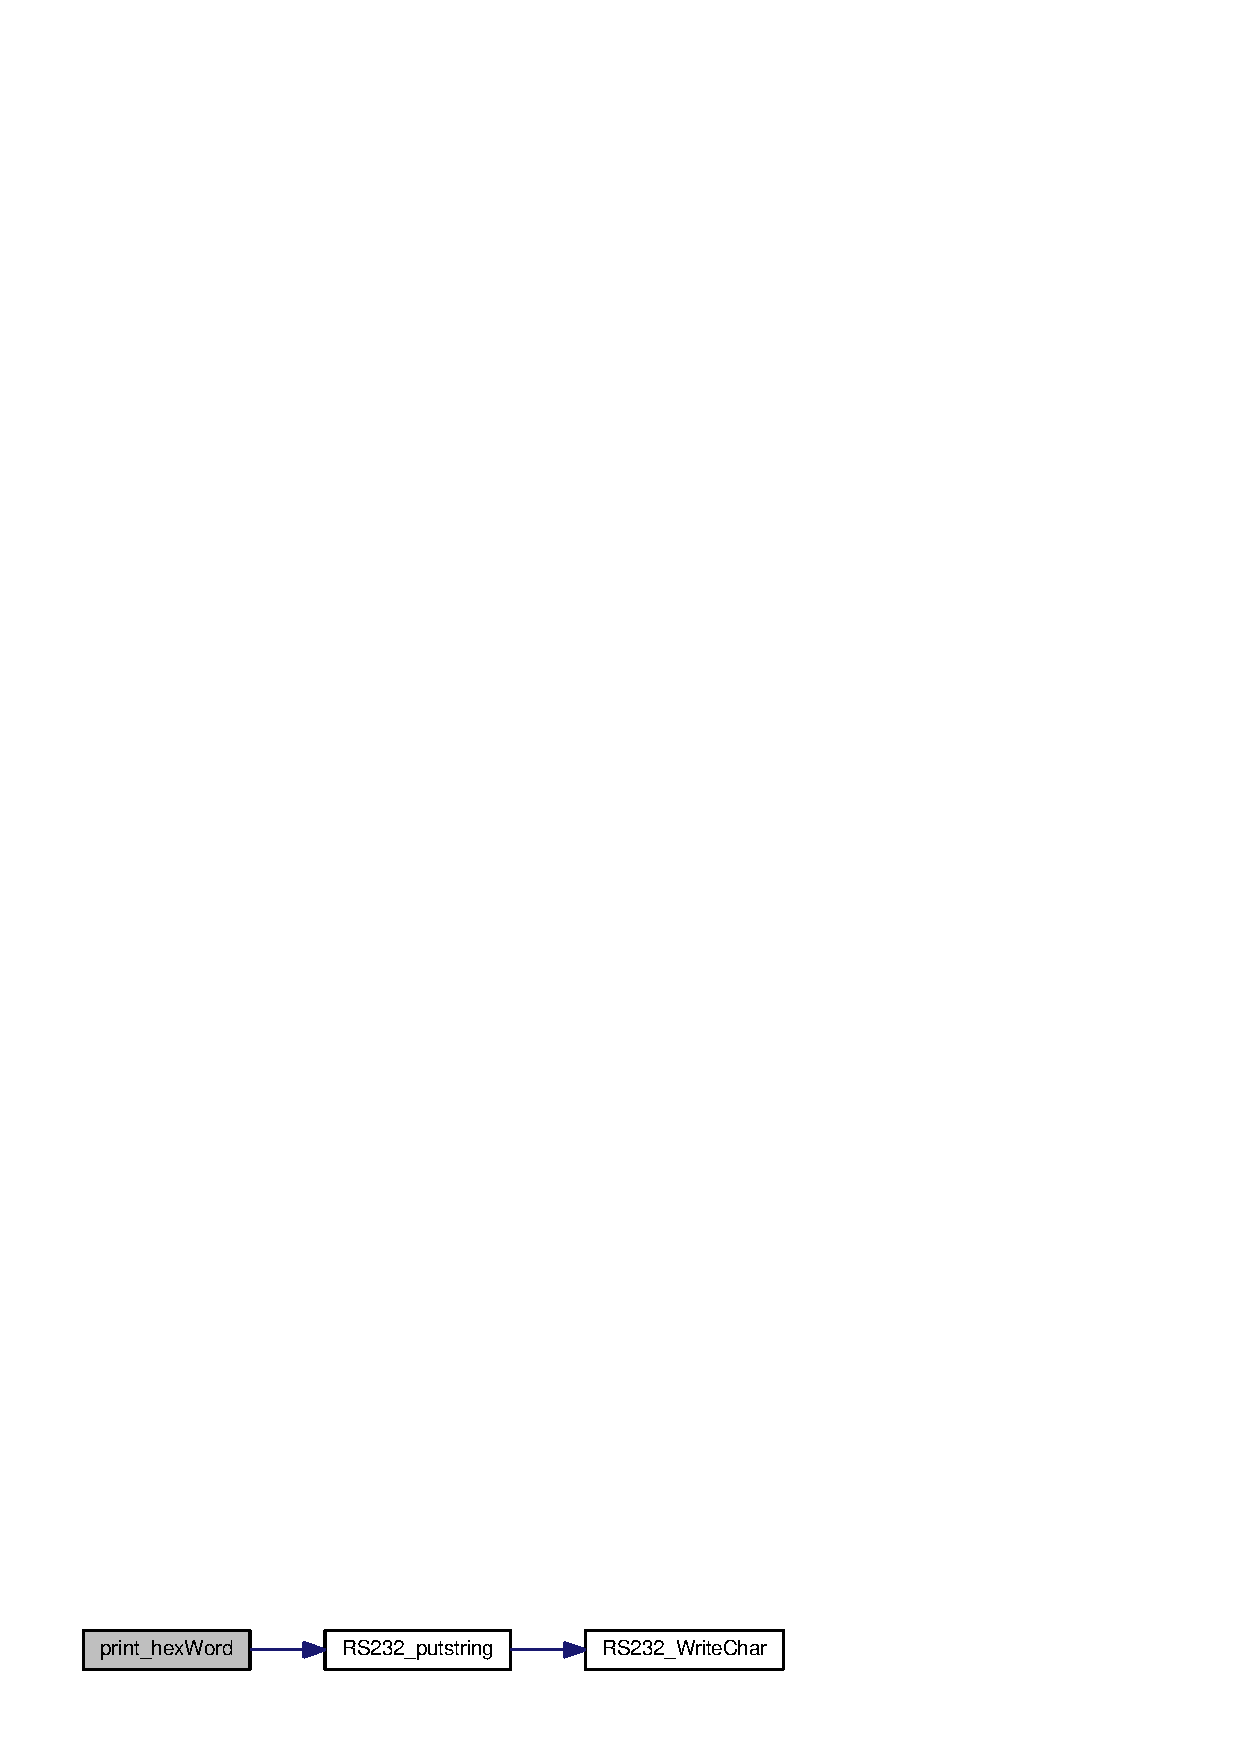
\includegraphics[width=350pt]{my_util_8c_a462f788430a8411cca8cfe2116118e31_cgraph}
\end{center}
\end{figure}


\index{my\+Util.\+c@{my\+Util.\+c}!print\+Str\+In\+Hex@{print\+Str\+In\+Hex}}
\index{print\+Str\+In\+Hex@{print\+Str\+In\+Hex}!my\+Util.\+c@{my\+Util.\+c}}
\subsubsection[{print\+Str\+In\+Hex(char $\ast$a\+String)}]{\setlength{\rightskip}{0pt plus 5cm}void print\+Str\+In\+Hex (
\begin{DoxyParamCaption}
\item[{char $\ast$}]{a\+String}
\end{DoxyParamCaption}
)}\label{my_util_8c_a6d7f0f873267ba014418802d89b68eb1}


Definition at line 169 of file my\+Util.\+c.



References print\+\_\+hex\+Byte().



Here is the call graph for this function\+:\nopagebreak
\begin{figure}[H]
\begin{center}
\leavevmode
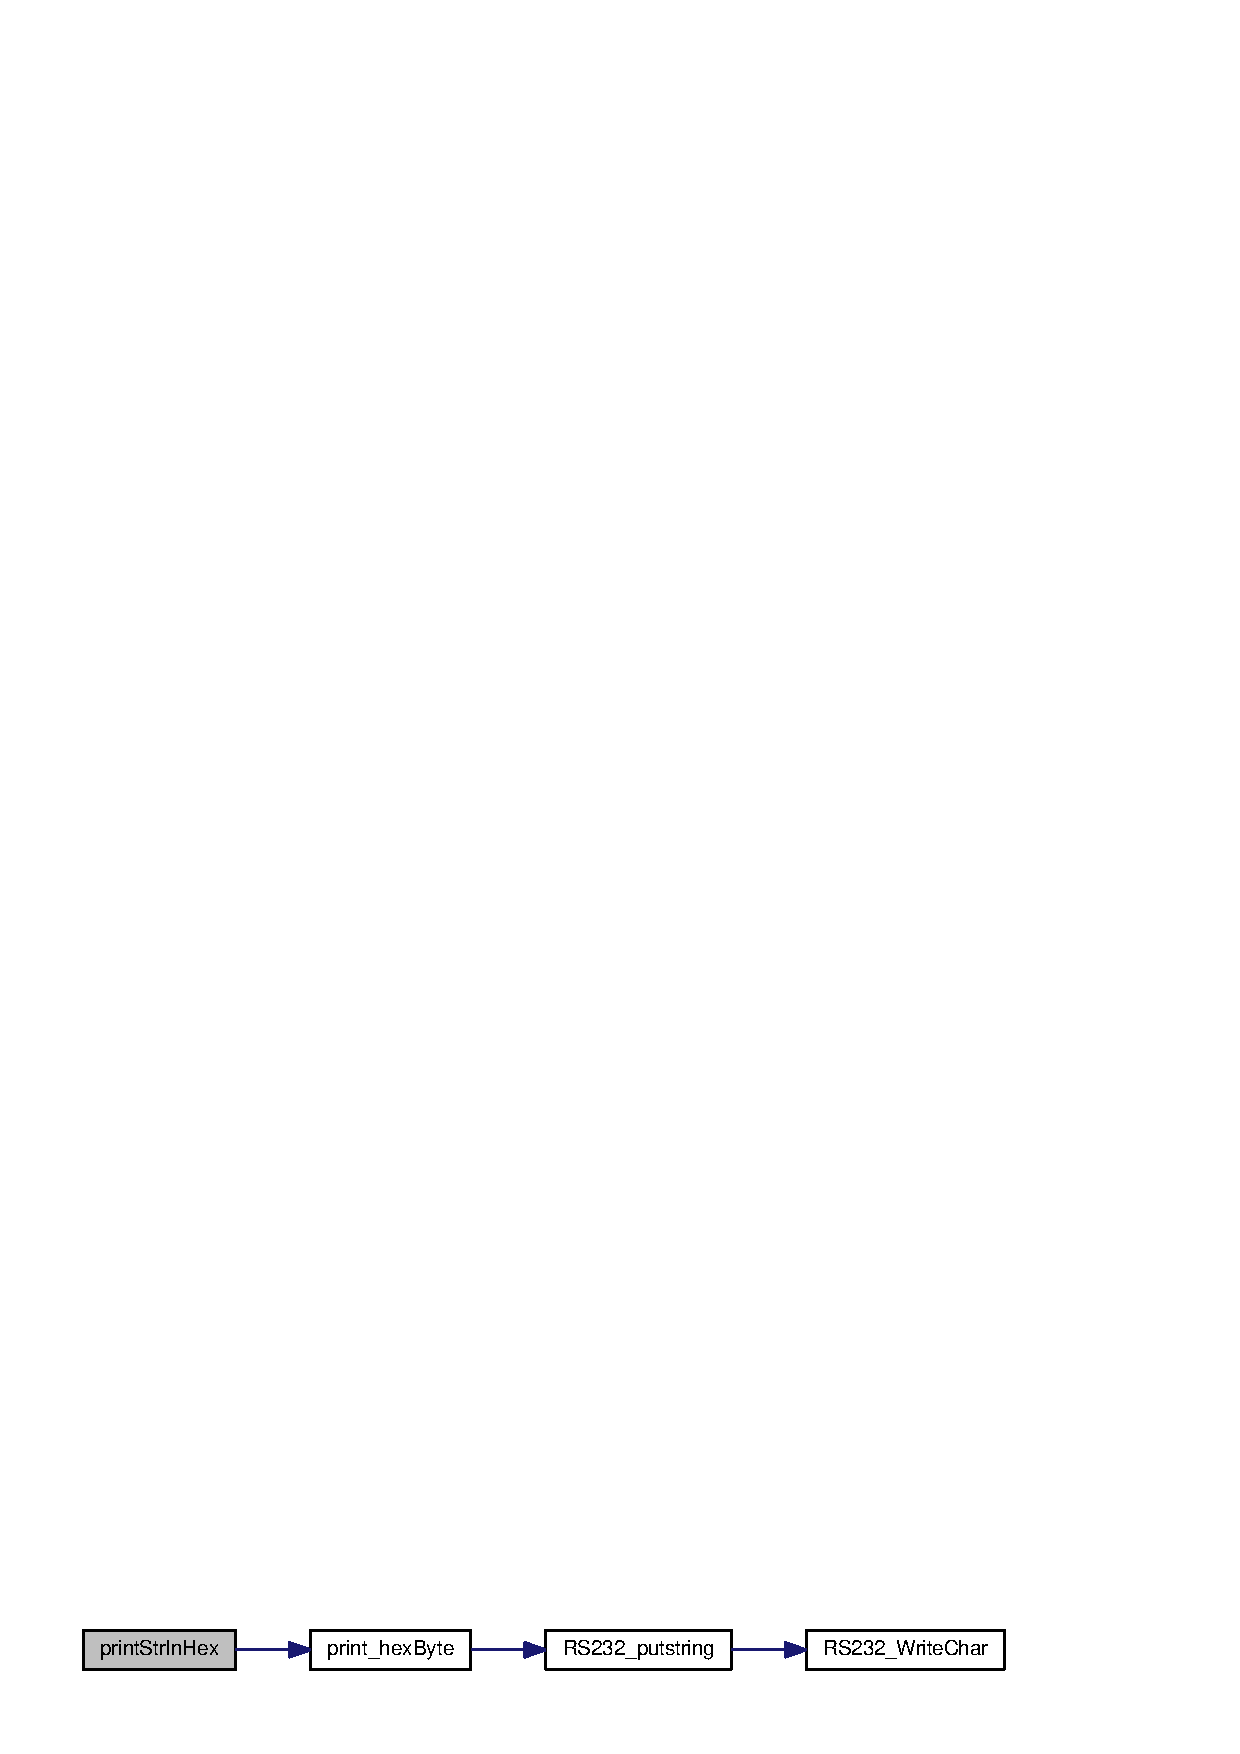
\includegraphics[width=350pt]{my_util_8c_a6d7f0f873267ba014418802d89b68eb1_cgraph}
\end{center}
\end{figure}



\section{U\+:/\+I\+C\+T/7th\+\_\+semester/bpri2/code/my\+Ethernut/rs485/src/my\+Util.h File Reference}
\label{my_util_8h}\index{U\+:/\+I\+C\+T/7th\+\_\+semester/bpri2/code/my\+Ethernut/rs485/src/my\+Util.\+h@{U\+:/\+I\+C\+T/7th\+\_\+semester/bpri2/code/my\+Ethernut/rs485/src/my\+Util.\+h}}
{\ttfamily \#include $<$avr/io.\+h$>$}\\*
{\ttfamily \#include $<$stdlib.\+h$>$}\\*
Include dependency graph for my\+Util.\+h\+:\nopagebreak
\begin{figure}[H]
\begin{center}
\leavevmode
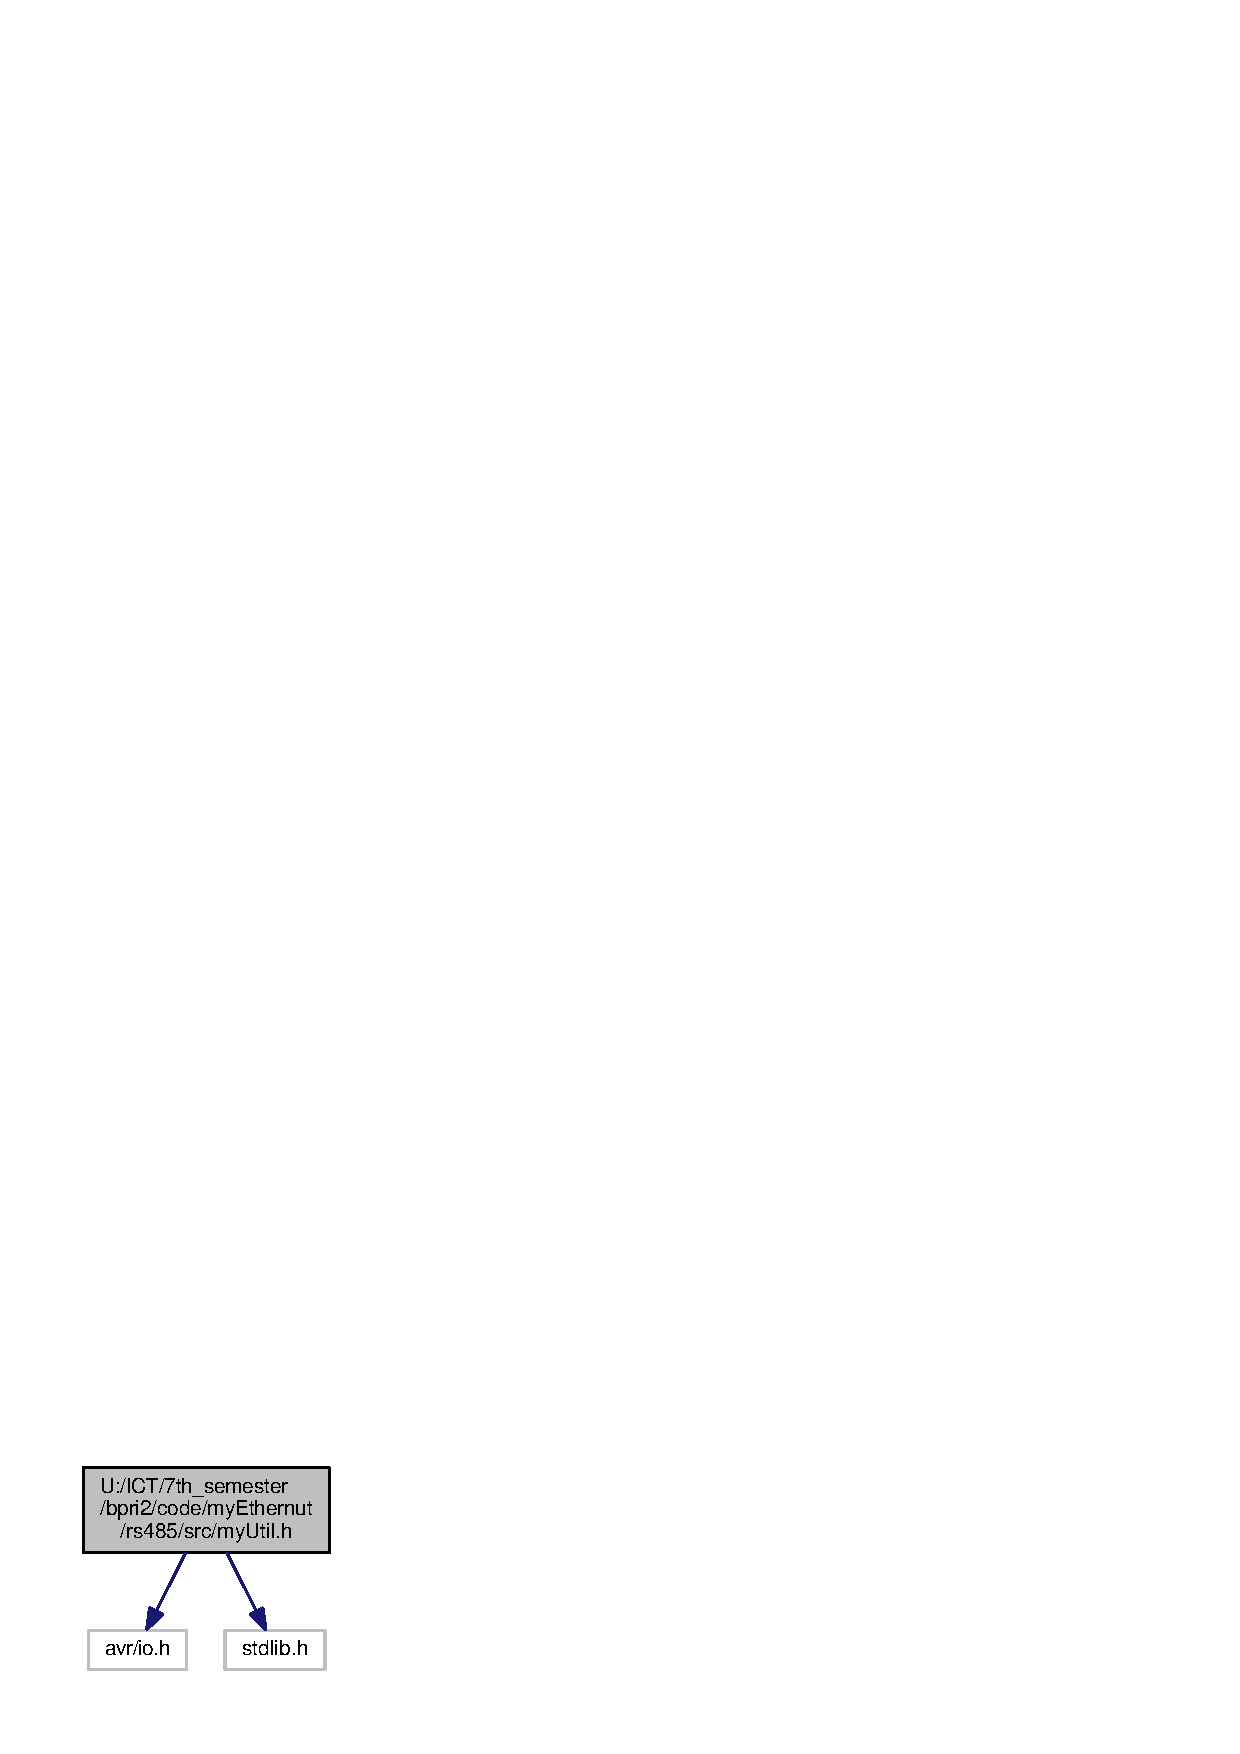
\includegraphics[width=162pt]{my_util_8h__incl}
\end{center}
\end{figure}
This graph shows which files directly or indirectly include this file\+:\nopagebreak
\begin{figure}[H]
\begin{center}
\leavevmode
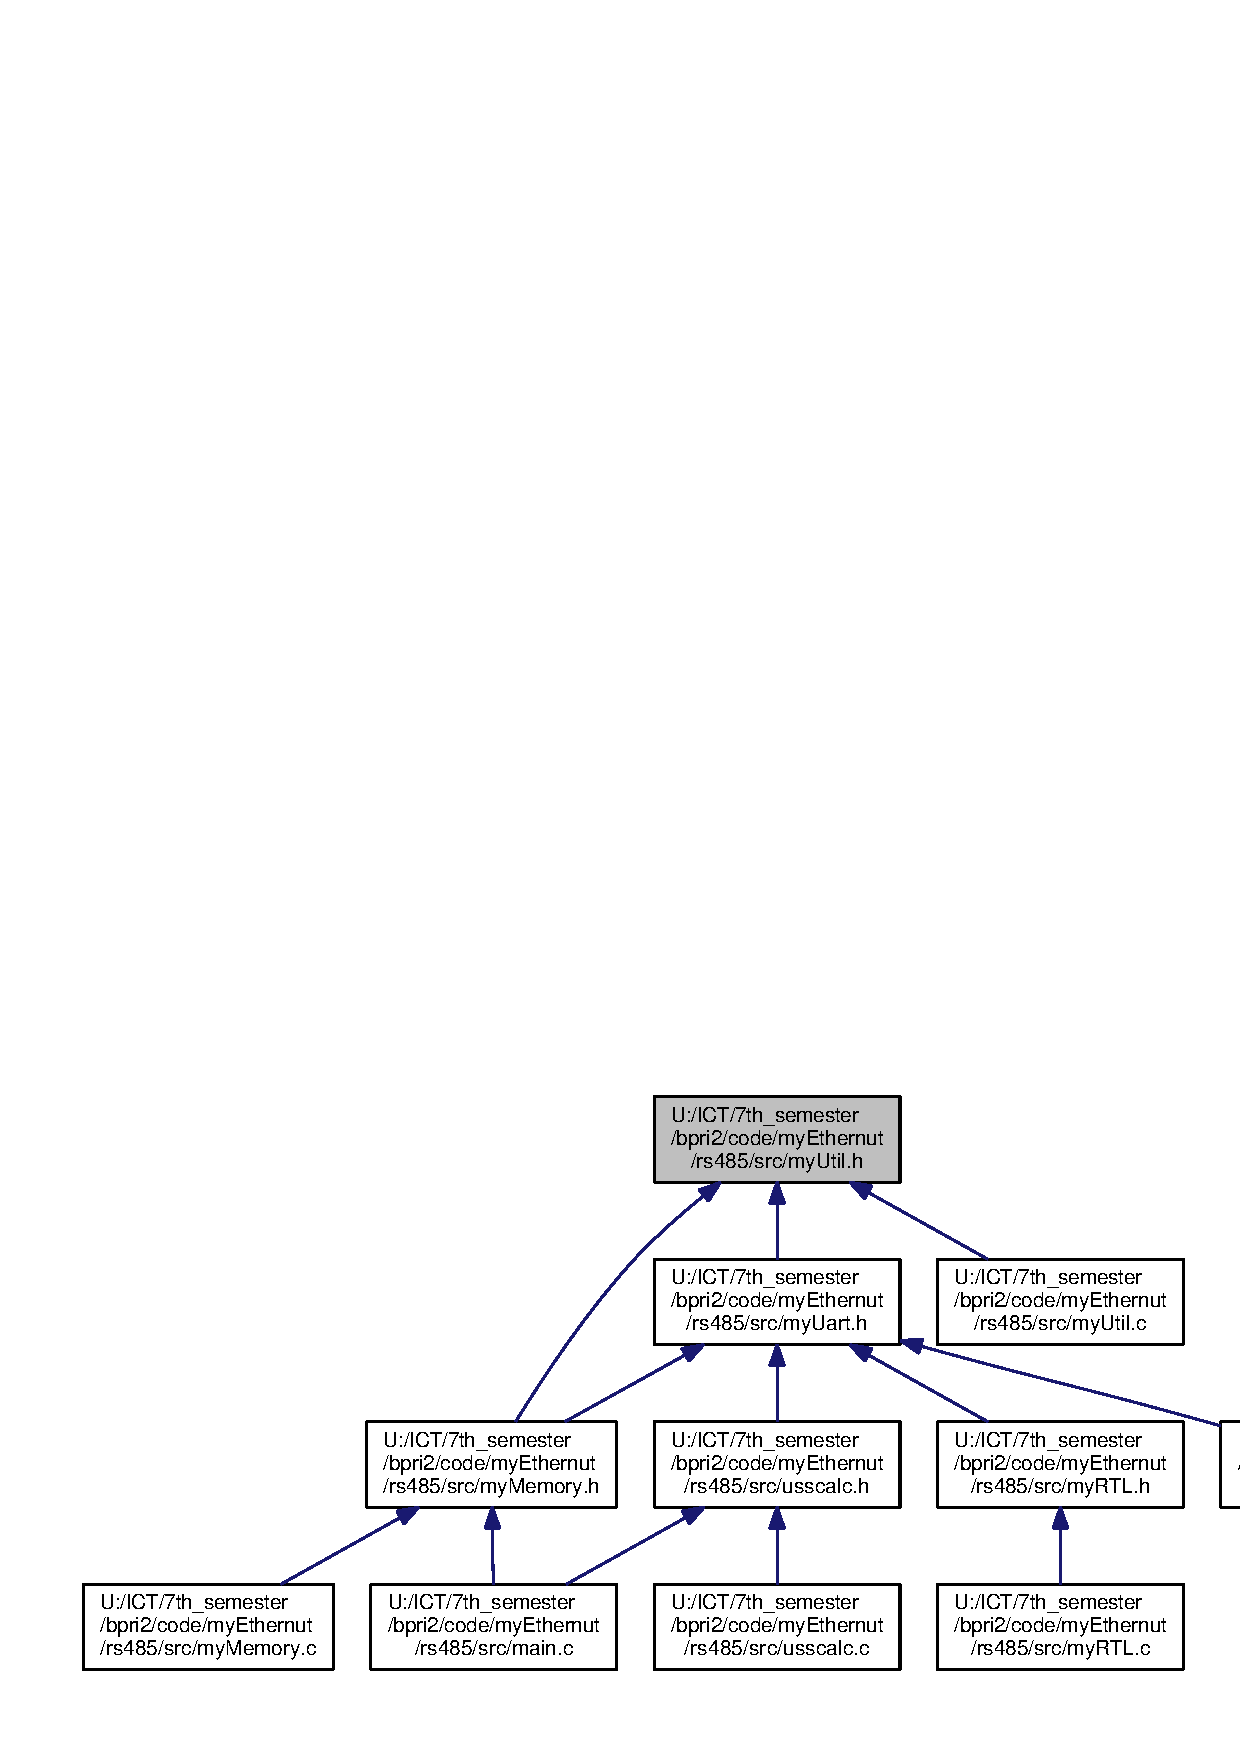
\includegraphics[width=350pt]{my_util_8h__dep__incl}
\end{center}
\end{figure}
\subsection*{Functions}
\begin{DoxyCompactItemize}
\item 
void {\bf print\+\_\+bin\+Byte} (uint8\+\_\+t my\+Byte)
\item 
void {\bf print\+\_\+hex\+Byte} (uint8\+\_\+t my\+Byte)
\item 
void {\bf print\+\_\+hex\+Word} (uint16\+\_\+t word)
\item 
void {\bf print\+\_\+hex\+Address} (uint16\+\_\+t address)
\item 
void {\bf print\+Str\+In\+Hex} (char $\ast$a\+String)
\item 
void {\bf deb\+\_\+print} (char $\ast$a\+String, uint8\+\_\+t byte)
\item 
void {\bf wait} (uint8\+\_\+t ile\+Nopuf)
\end{DoxyCompactItemize}


\subsection{Function Documentation}
\index{my\+Util.\+h@{my\+Util.\+h}!deb\+\_\+print@{deb\+\_\+print}}
\index{deb\+\_\+print@{deb\+\_\+print}!my\+Util.\+h@{my\+Util.\+h}}
\subsubsection[{deb\+\_\+print(char $\ast$a\+String, uint8\+\_\+t byte)}]{\setlength{\rightskip}{0pt plus 5cm}void deb\+\_\+print (
\begin{DoxyParamCaption}
\item[{char $\ast$}]{a\+String, }
\item[{uint8\+\_\+t}]{byte}
\end{DoxyParamCaption}
)}\label{my_util_8h_a2f9f5b067182da7e5194b95dd69796d5}


Definition at line 179 of file my\+Util.\+c.



References R\+S232\+\_\+putstring().



Here is the call graph for this function\+:\nopagebreak
\begin{figure}[H]
\begin{center}
\leavevmode
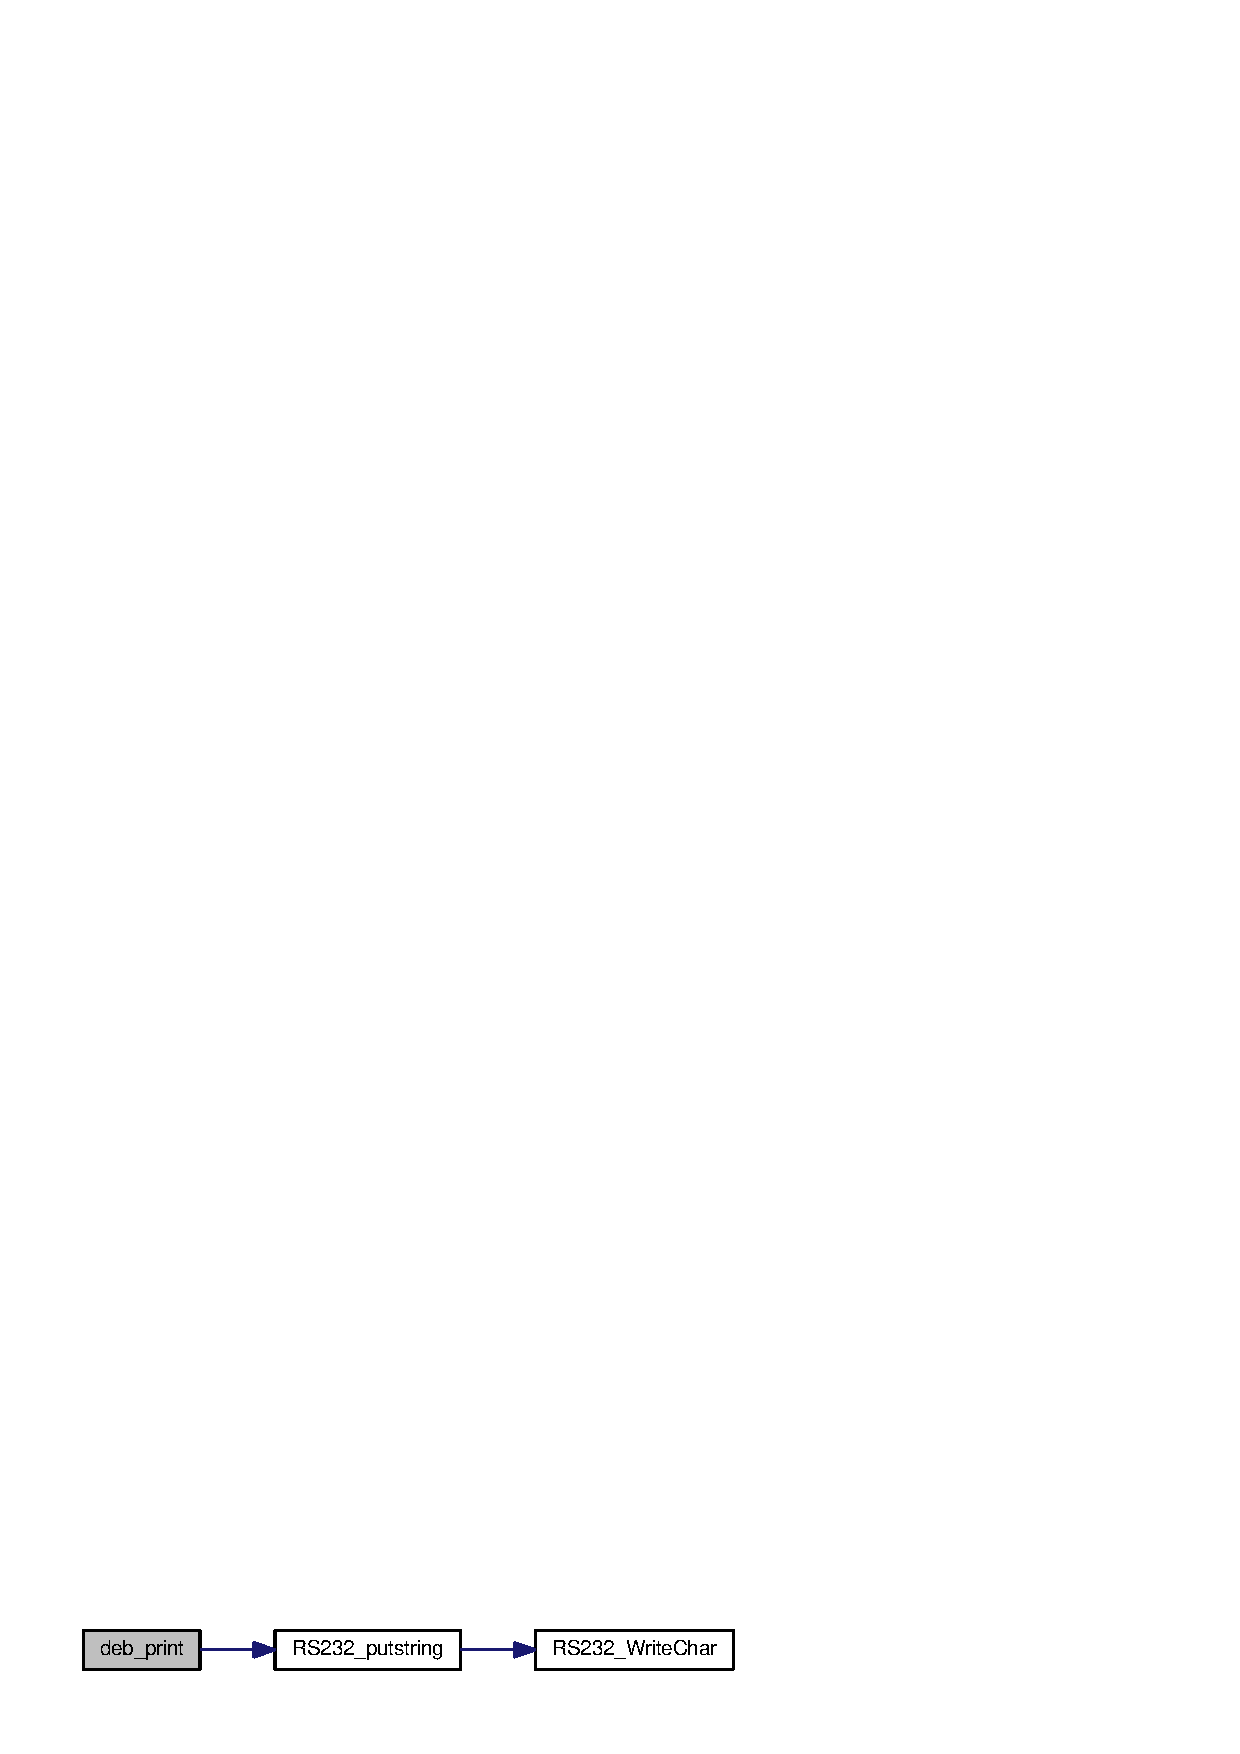
\includegraphics[width=350pt]{my_util_8h_a2f9f5b067182da7e5194b95dd69796d5_cgraph}
\end{center}
\end{figure}


\index{my\+Util.\+h@{my\+Util.\+h}!print\+\_\+bin\+Byte@{print\+\_\+bin\+Byte}}
\index{print\+\_\+bin\+Byte@{print\+\_\+bin\+Byte}!my\+Util.\+h@{my\+Util.\+h}}
\subsubsection[{print\+\_\+bin\+Byte(uint8\+\_\+t my\+Byte)}]{\setlength{\rightskip}{0pt plus 5cm}void print\+\_\+bin\+Byte (
\begin{DoxyParamCaption}
\item[{uint8\+\_\+t}]{my\+Byte}
\end{DoxyParamCaption}
)}\label{my_util_8h_a446d5fa92eead663eb3c401c3728b49f}


Definition at line 16 of file my\+Util.\+c.



References R\+S232\+\_\+putstring(), and R\+S232\+\_\+\+Write\+Char().



Here is the call graph for this function\+:\nopagebreak
\begin{figure}[H]
\begin{center}
\leavevmode
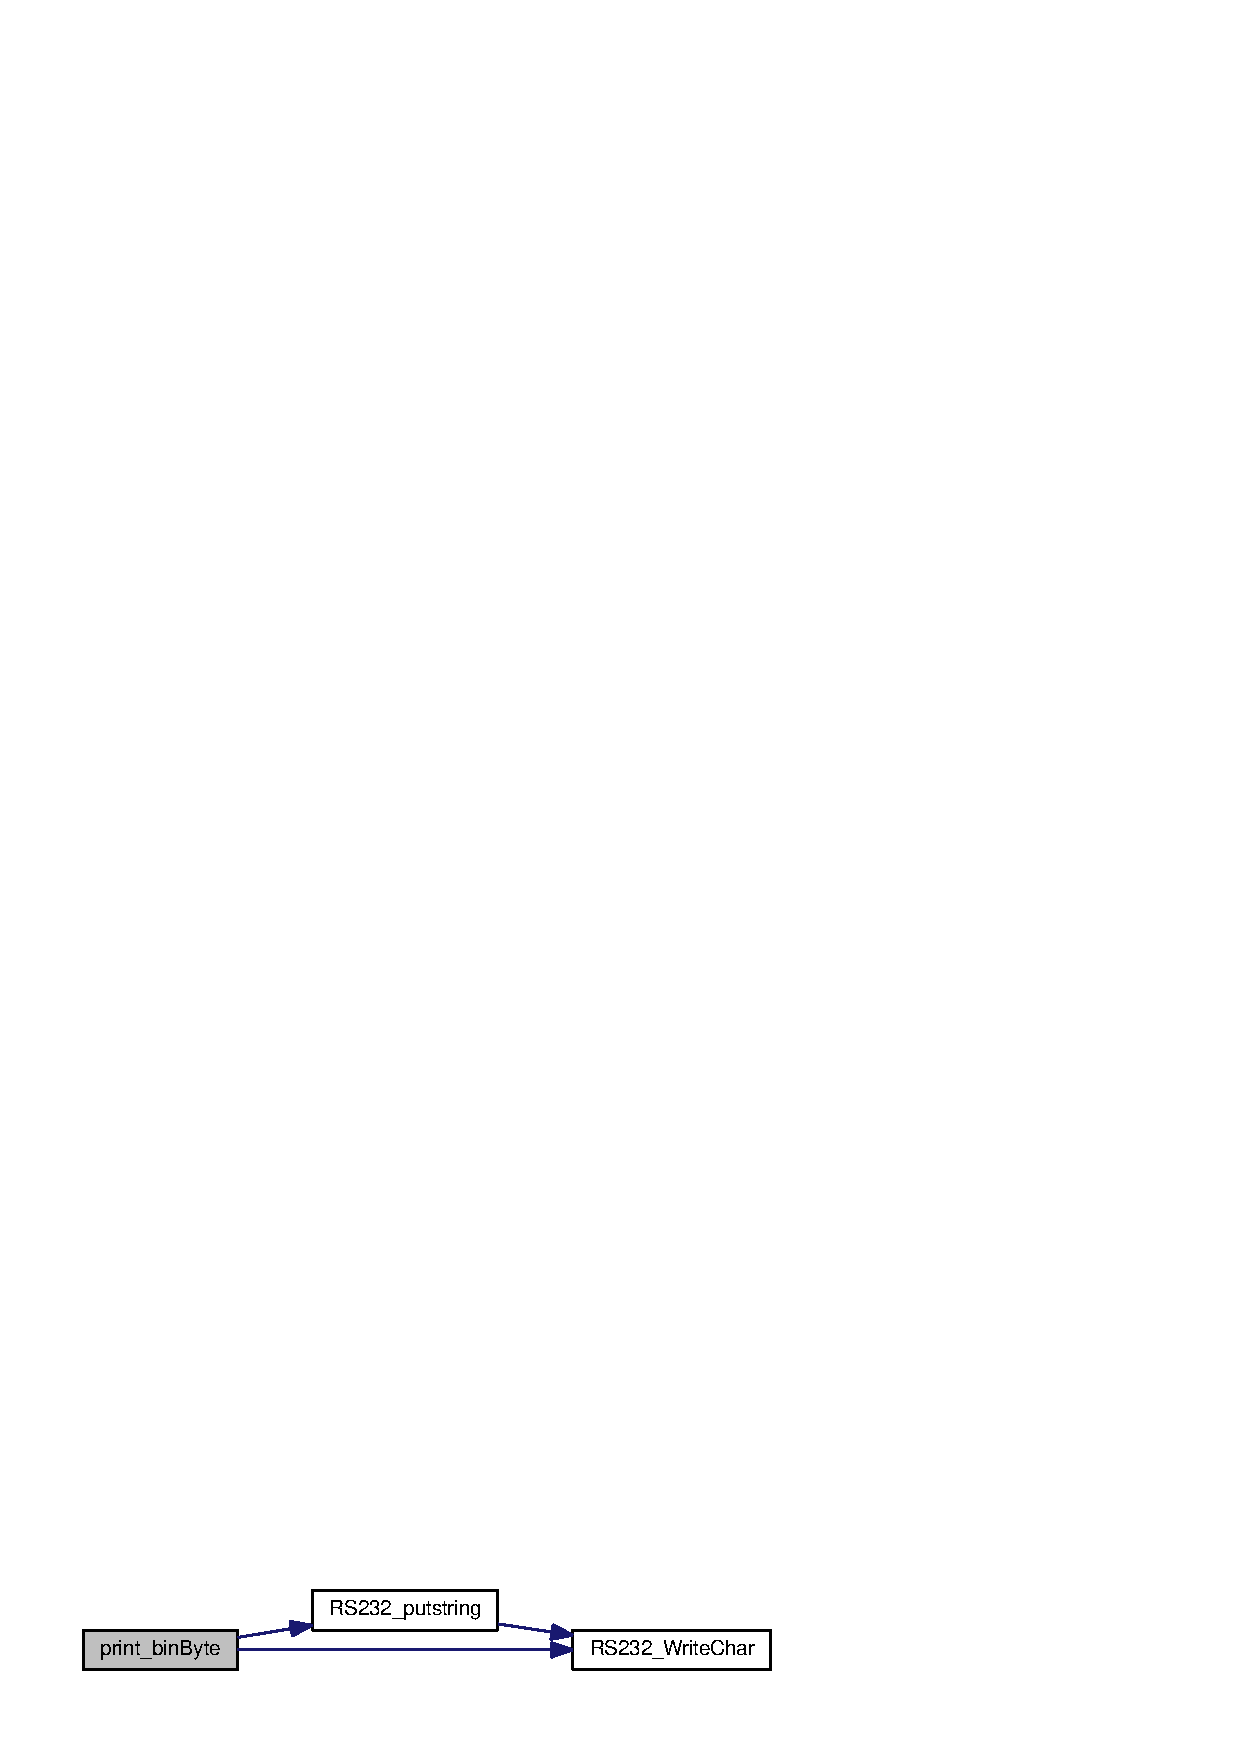
\includegraphics[width=350pt]{my_util_8h_a446d5fa92eead663eb3c401c3728b49f_cgraph}
\end{center}
\end{figure}


\index{my\+Util.\+h@{my\+Util.\+h}!print\+\_\+hex\+Address@{print\+\_\+hex\+Address}}
\index{print\+\_\+hex\+Address@{print\+\_\+hex\+Address}!my\+Util.\+h@{my\+Util.\+h}}
\subsubsection[{print\+\_\+hex\+Address(uint16\+\_\+t address)}]{\setlength{\rightskip}{0pt plus 5cm}void print\+\_\+hex\+Address (
\begin{DoxyParamCaption}
\item[{uint16\+\_\+t}]{address}
\end{DoxyParamCaption}
)}\label{my_util_8h_afb61822546c6e61b88e5e165764a3ccb}


Definition at line 109 of file my\+Util.\+c.



References R\+S232\+\_\+putstring().



Referenced by read\+R\+T\+L\+Memory(), and test\+Memory().



Here is the call graph for this function\+:\nopagebreak
\begin{figure}[H]
\begin{center}
\leavevmode
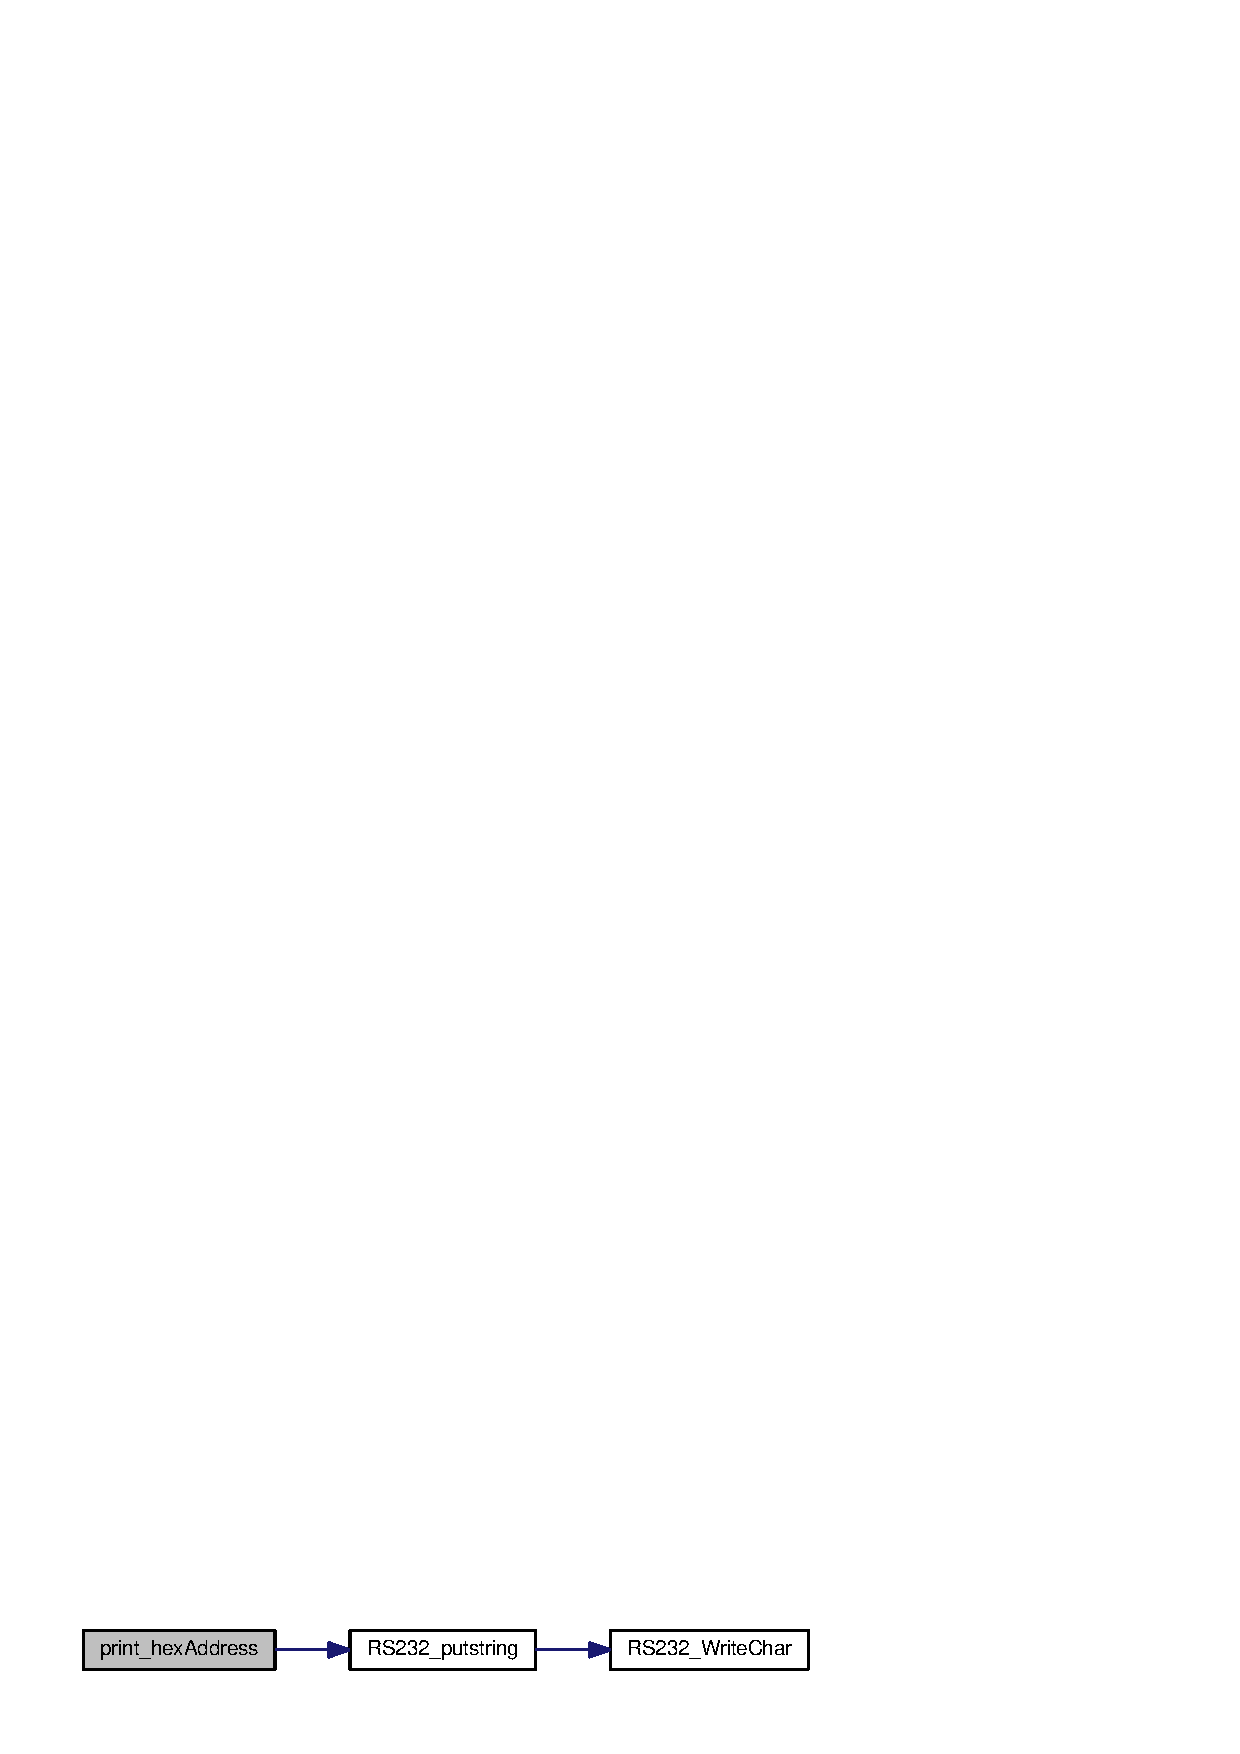
\includegraphics[width=350pt]{my_util_8h_afb61822546c6e61b88e5e165764a3ccb_cgraph}
\end{center}
\end{figure}


\index{my\+Util.\+h@{my\+Util.\+h}!print\+\_\+hex\+Byte@{print\+\_\+hex\+Byte}}
\index{print\+\_\+hex\+Byte@{print\+\_\+hex\+Byte}!my\+Util.\+h@{my\+Util.\+h}}
\subsubsection[{print\+\_\+hex\+Byte(uint8\+\_\+t my\+Byte)}]{\setlength{\rightskip}{0pt plus 5cm}void print\+\_\+hex\+Byte (
\begin{DoxyParamCaption}
\item[{uint8\+\_\+t}]{my\+Byte}
\end{DoxyParamCaption}
)}\label{my_util_8h_aebd073f6dad448b0012eef8a8fd982fb}


Definition at line 35 of file my\+Util.\+c.



References R\+S232\+\_\+putstring().



Referenced by display\+Telegram(), print\+Str\+In\+Hex(), and Test\+External\+Ram().



Here is the call graph for this function\+:\nopagebreak
\begin{figure}[H]
\begin{center}
\leavevmode
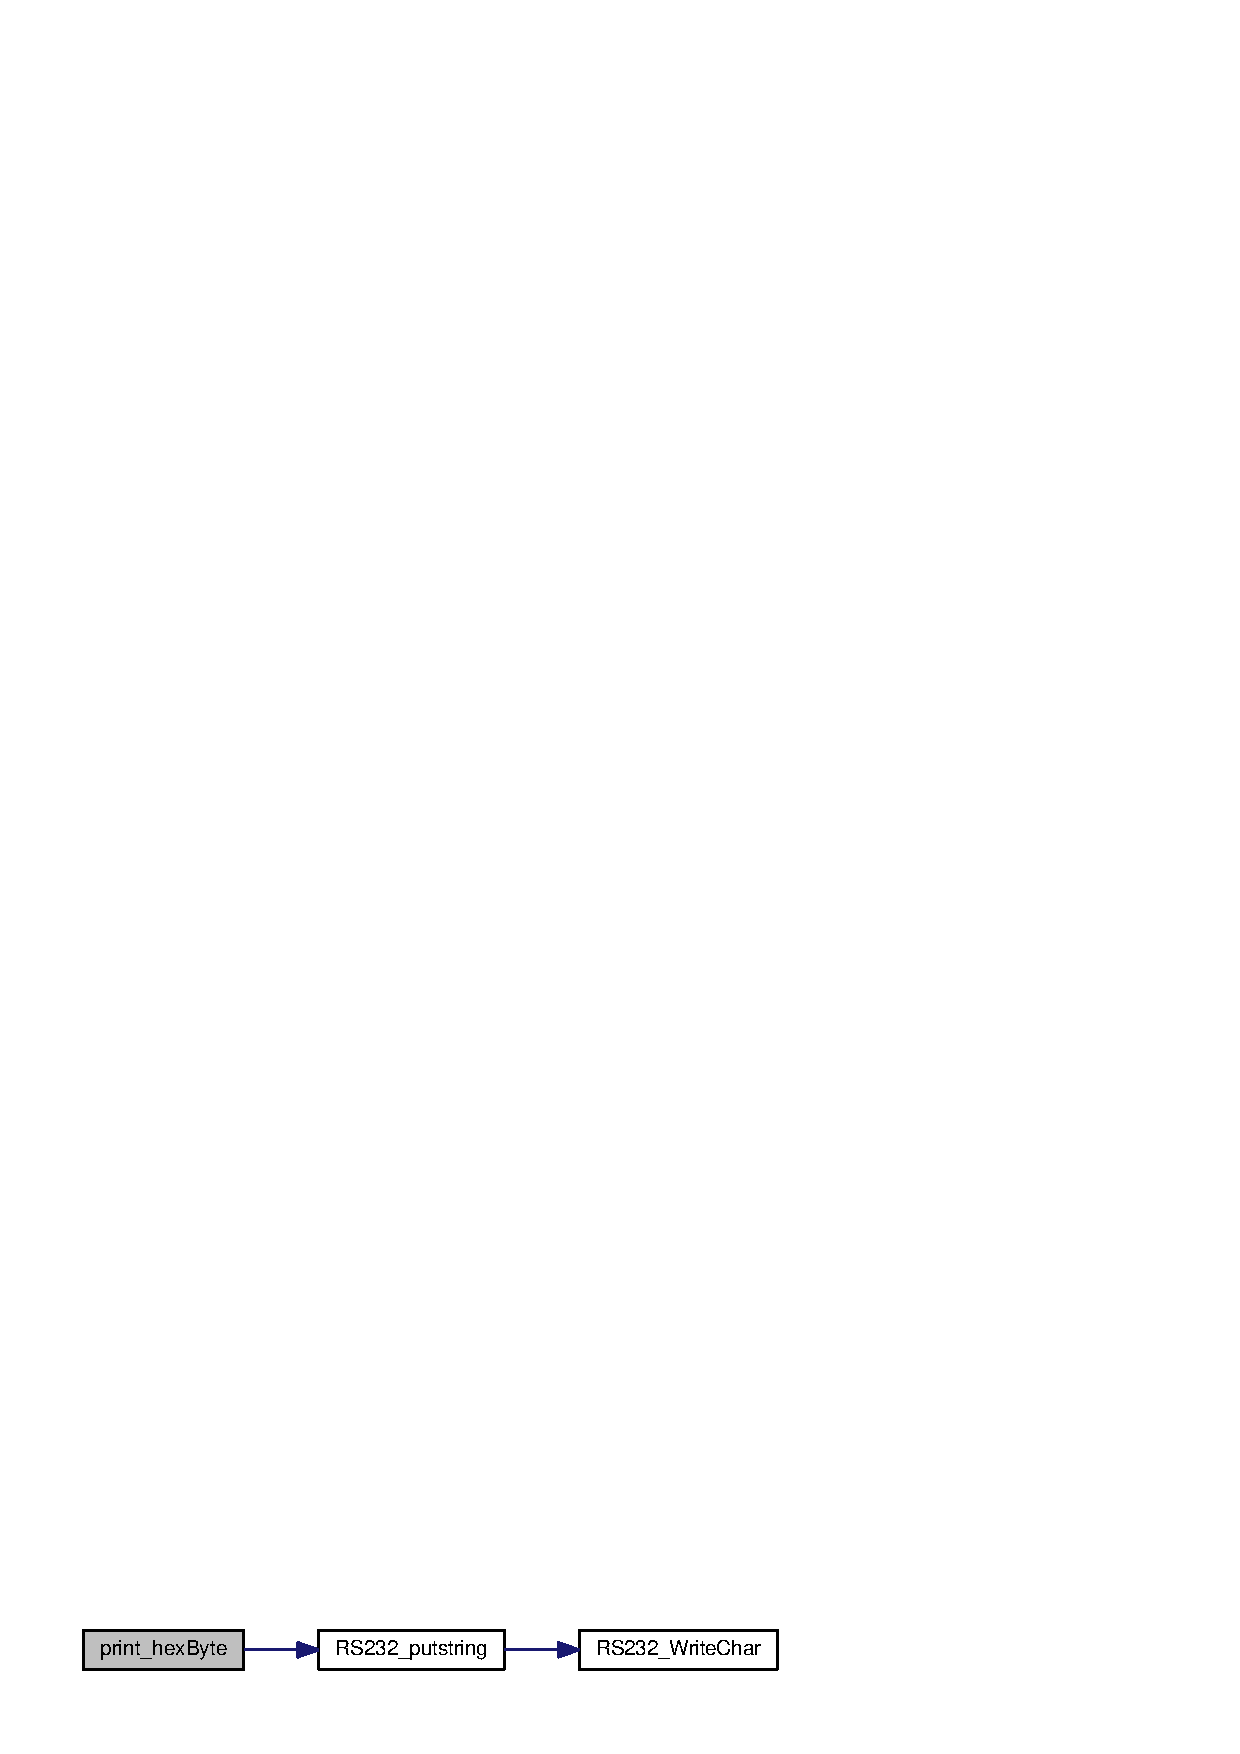
\includegraphics[width=350pt]{my_util_8h_aebd073f6dad448b0012eef8a8fd982fb_cgraph}
\end{center}
\end{figure}


\index{my\+Util.\+h@{my\+Util.\+h}!print\+\_\+hex\+Word@{print\+\_\+hex\+Word}}
\index{print\+\_\+hex\+Word@{print\+\_\+hex\+Word}!my\+Util.\+h@{my\+Util.\+h}}
\subsubsection[{print\+\_\+hex\+Word(uint16\+\_\+t word)}]{\setlength{\rightskip}{0pt plus 5cm}void print\+\_\+hex\+Word (
\begin{DoxyParamCaption}
\item[{uint16\+\_\+t}]{word}
\end{DoxyParamCaption}
)}\label{my_util_8h_a6ef50603ed9300df8de507aa203c8b67}


Definition at line 49 of file my\+Util.\+c.



References R\+S232\+\_\+putstring().



Referenced by main(), read\+R\+T\+L\+Memory(), test\+Memory(), and Test\+Realtek().



Here is the call graph for this function\+:\nopagebreak
\begin{figure}[H]
\begin{center}
\leavevmode
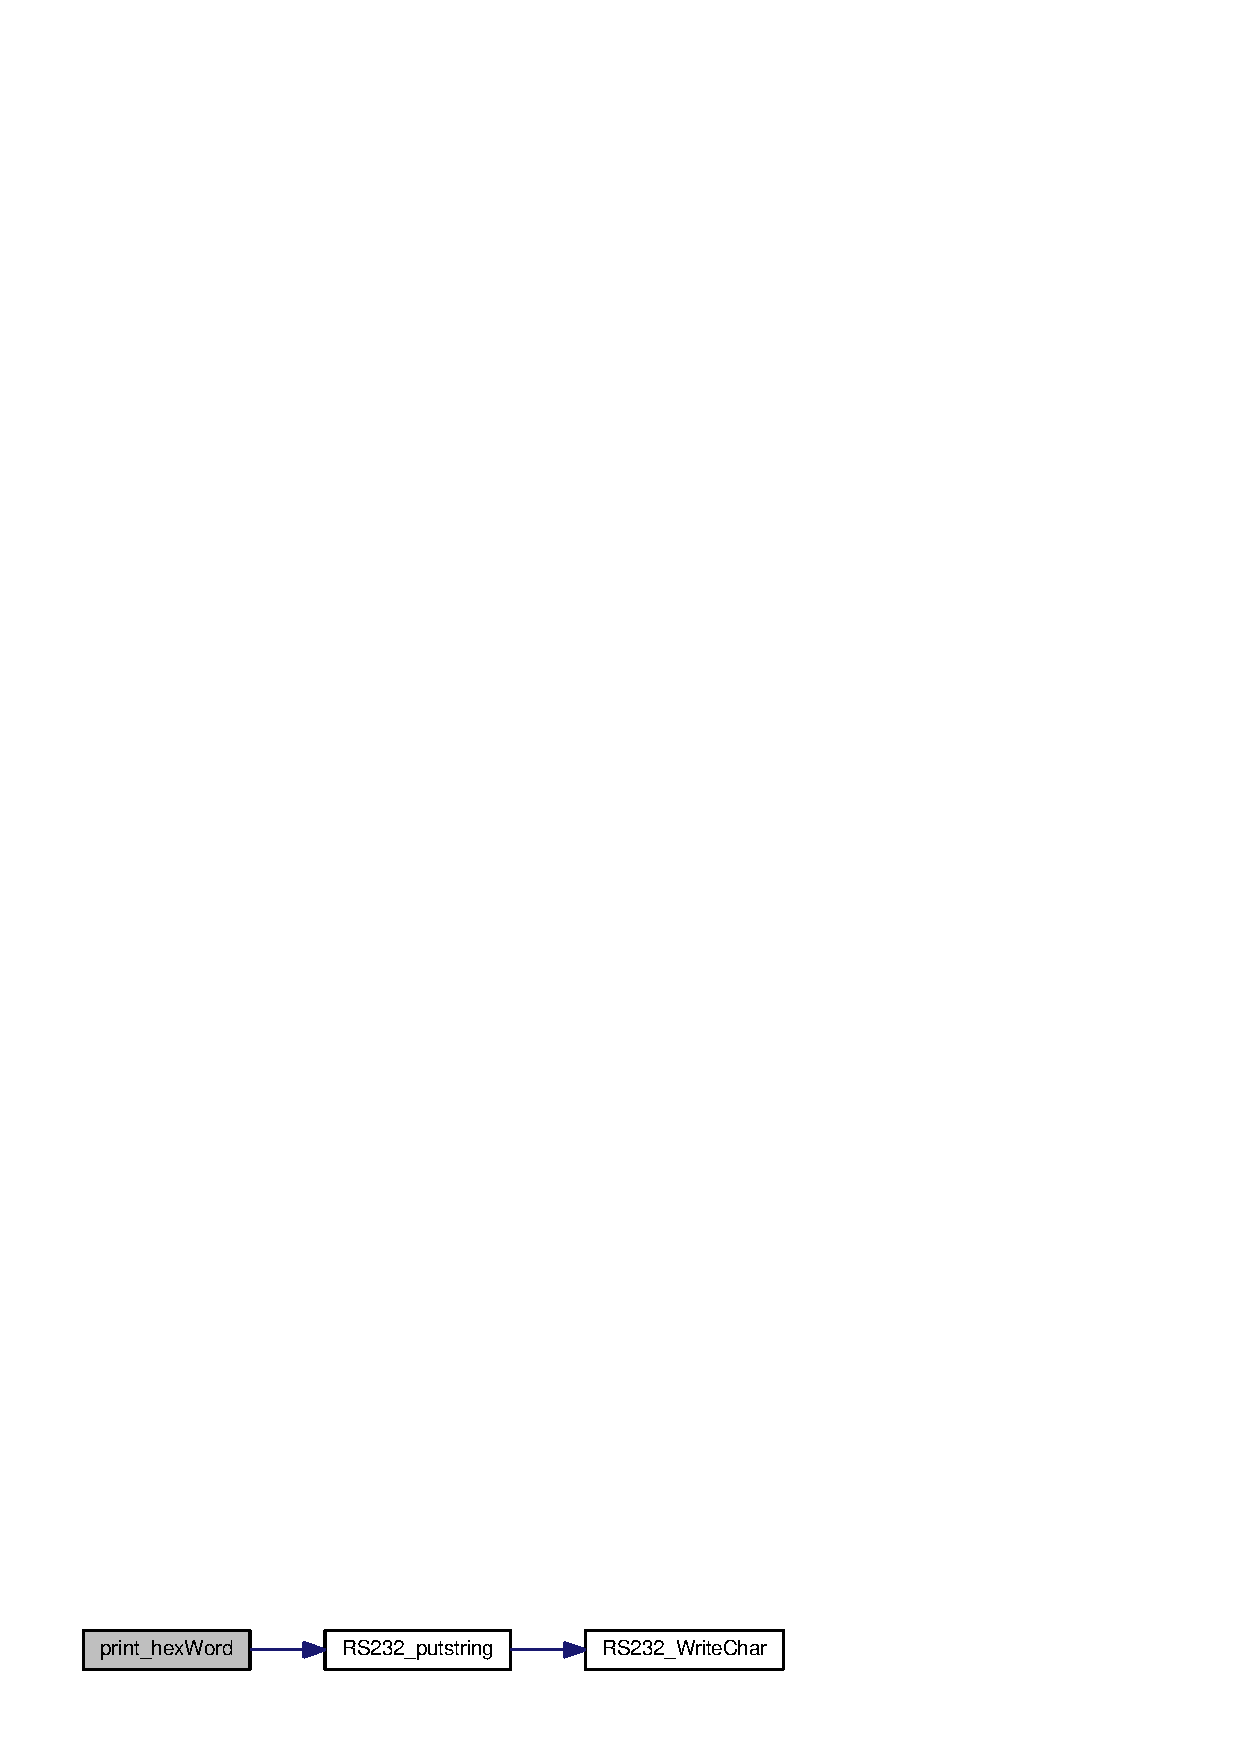
\includegraphics[width=350pt]{my_util_8h_a6ef50603ed9300df8de507aa203c8b67_cgraph}
\end{center}
\end{figure}


\index{my\+Util.\+h@{my\+Util.\+h}!print\+Str\+In\+Hex@{print\+Str\+In\+Hex}}
\index{print\+Str\+In\+Hex@{print\+Str\+In\+Hex}!my\+Util.\+h@{my\+Util.\+h}}
\subsubsection[{print\+Str\+In\+Hex(char $\ast$a\+String)}]{\setlength{\rightskip}{0pt plus 5cm}void print\+Str\+In\+Hex (
\begin{DoxyParamCaption}
\item[{char $\ast$}]{a\+String}
\end{DoxyParamCaption}
)}\label{my_util_8h_a6d7f0f873267ba014418802d89b68eb1}


Definition at line 169 of file my\+Util.\+c.



References print\+\_\+hex\+Byte().



Here is the call graph for this function\+:\nopagebreak
\begin{figure}[H]
\begin{center}
\leavevmode
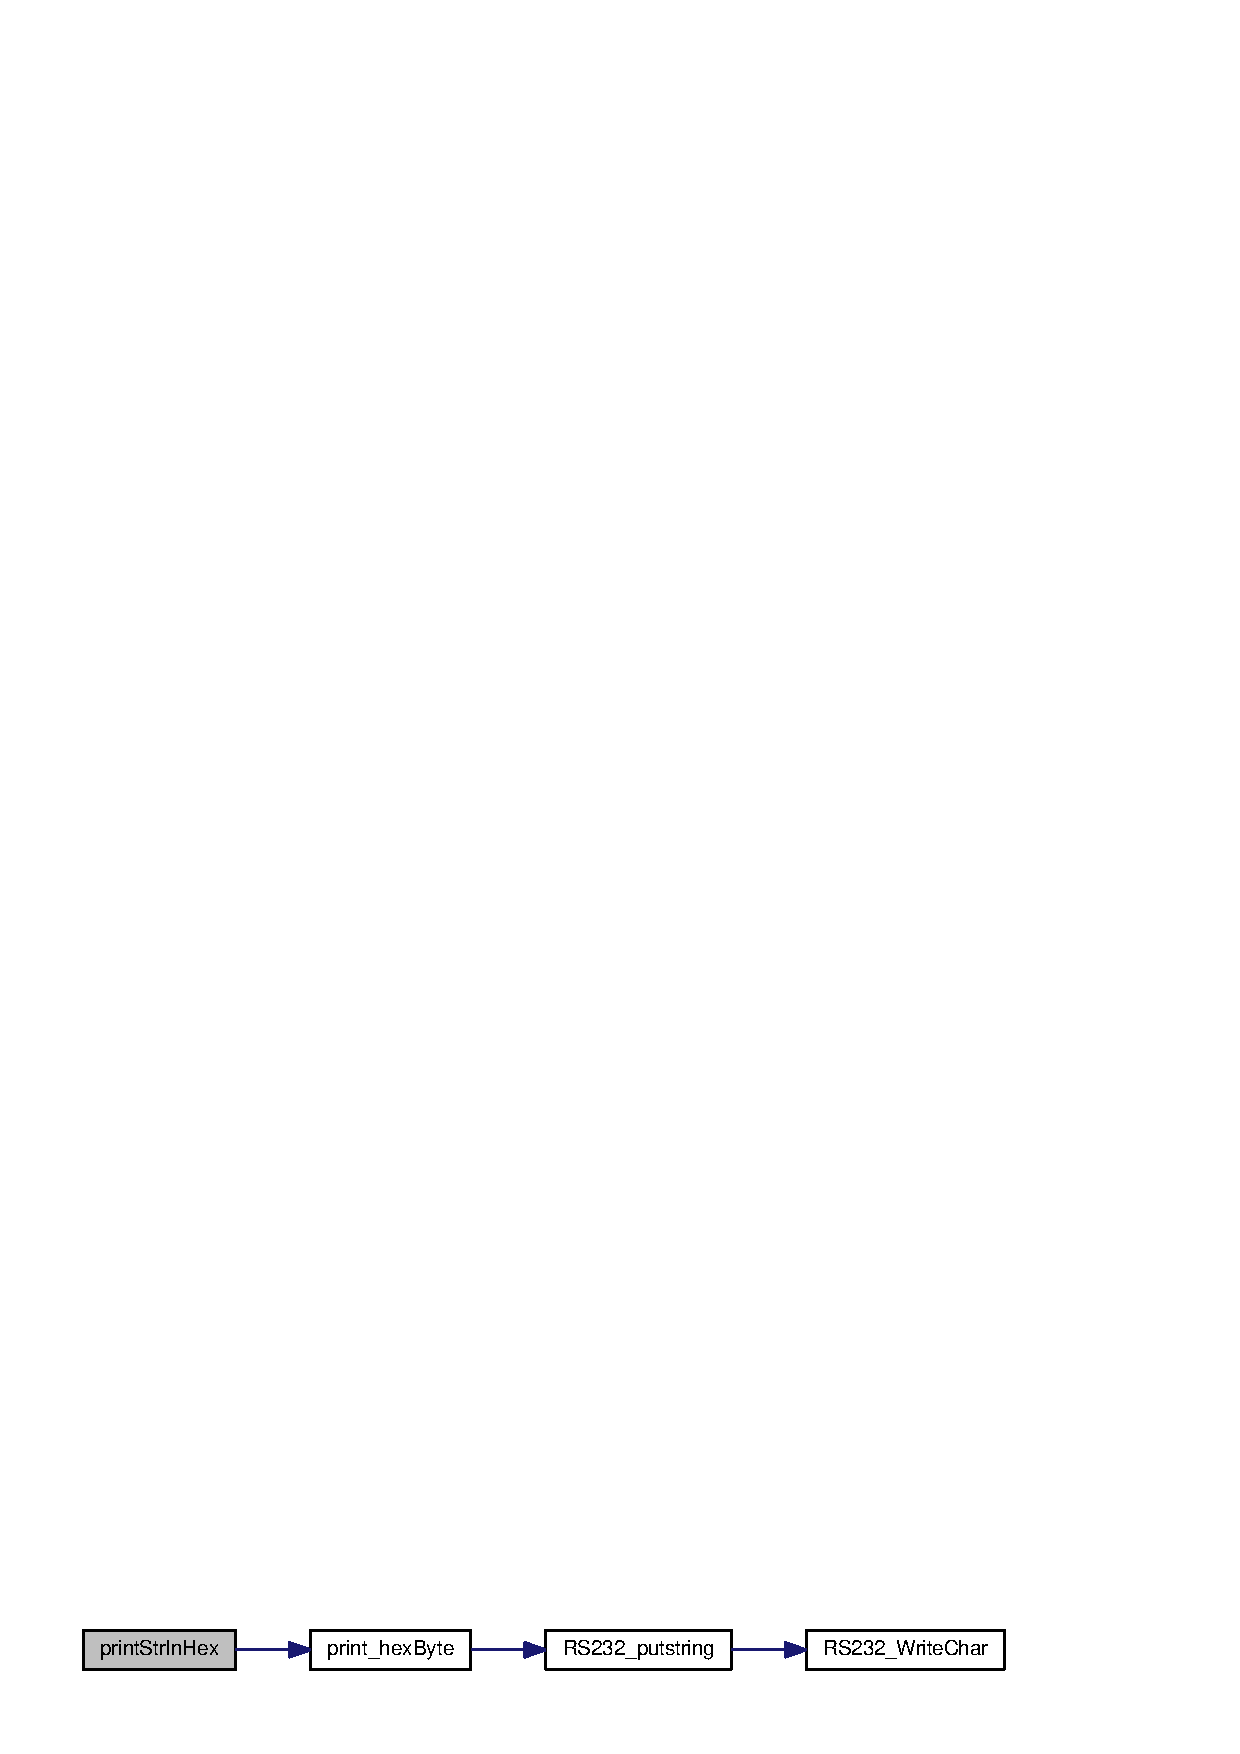
\includegraphics[width=350pt]{my_util_8h_a6d7f0f873267ba014418802d89b68eb1_cgraph}
\end{center}
\end{figure}


\index{my\+Util.\+h@{my\+Util.\+h}!wait@{wait}}
\index{wait@{wait}!my\+Util.\+h@{my\+Util.\+h}}
\subsubsection[{wait(uint8\+\_\+t ile\+Nopuf)}]{\setlength{\rightskip}{0pt plus 5cm}void wait (
\begin{DoxyParamCaption}
\item[{uint8\+\_\+t}]{ile\+Nopuf}
\end{DoxyParamCaption}
)}\label{my_util_8h_a8af1ec38872046061852770e1d6e7ebd}

\section{U\+:/\+I\+C\+T/7th\+\_\+semester/bpri2/code/my\+Ethernut/rs485/src/usscalc.c File Reference}
\label{usscalc_8c}\index{U\+:/\+I\+C\+T/7th\+\_\+semester/bpri2/code/my\+Ethernut/rs485/src/usscalc.\+c@{U\+:/\+I\+C\+T/7th\+\_\+semester/bpri2/code/my\+Ethernut/rs485/src/usscalc.\+c}}
{\ttfamily \#include \char`\"{}usscalc.\+h\char`\"{}}\\*
Include dependency graph for usscalc.\+c\+:\nopagebreak
\begin{figure}[H]
\begin{center}
\leavevmode
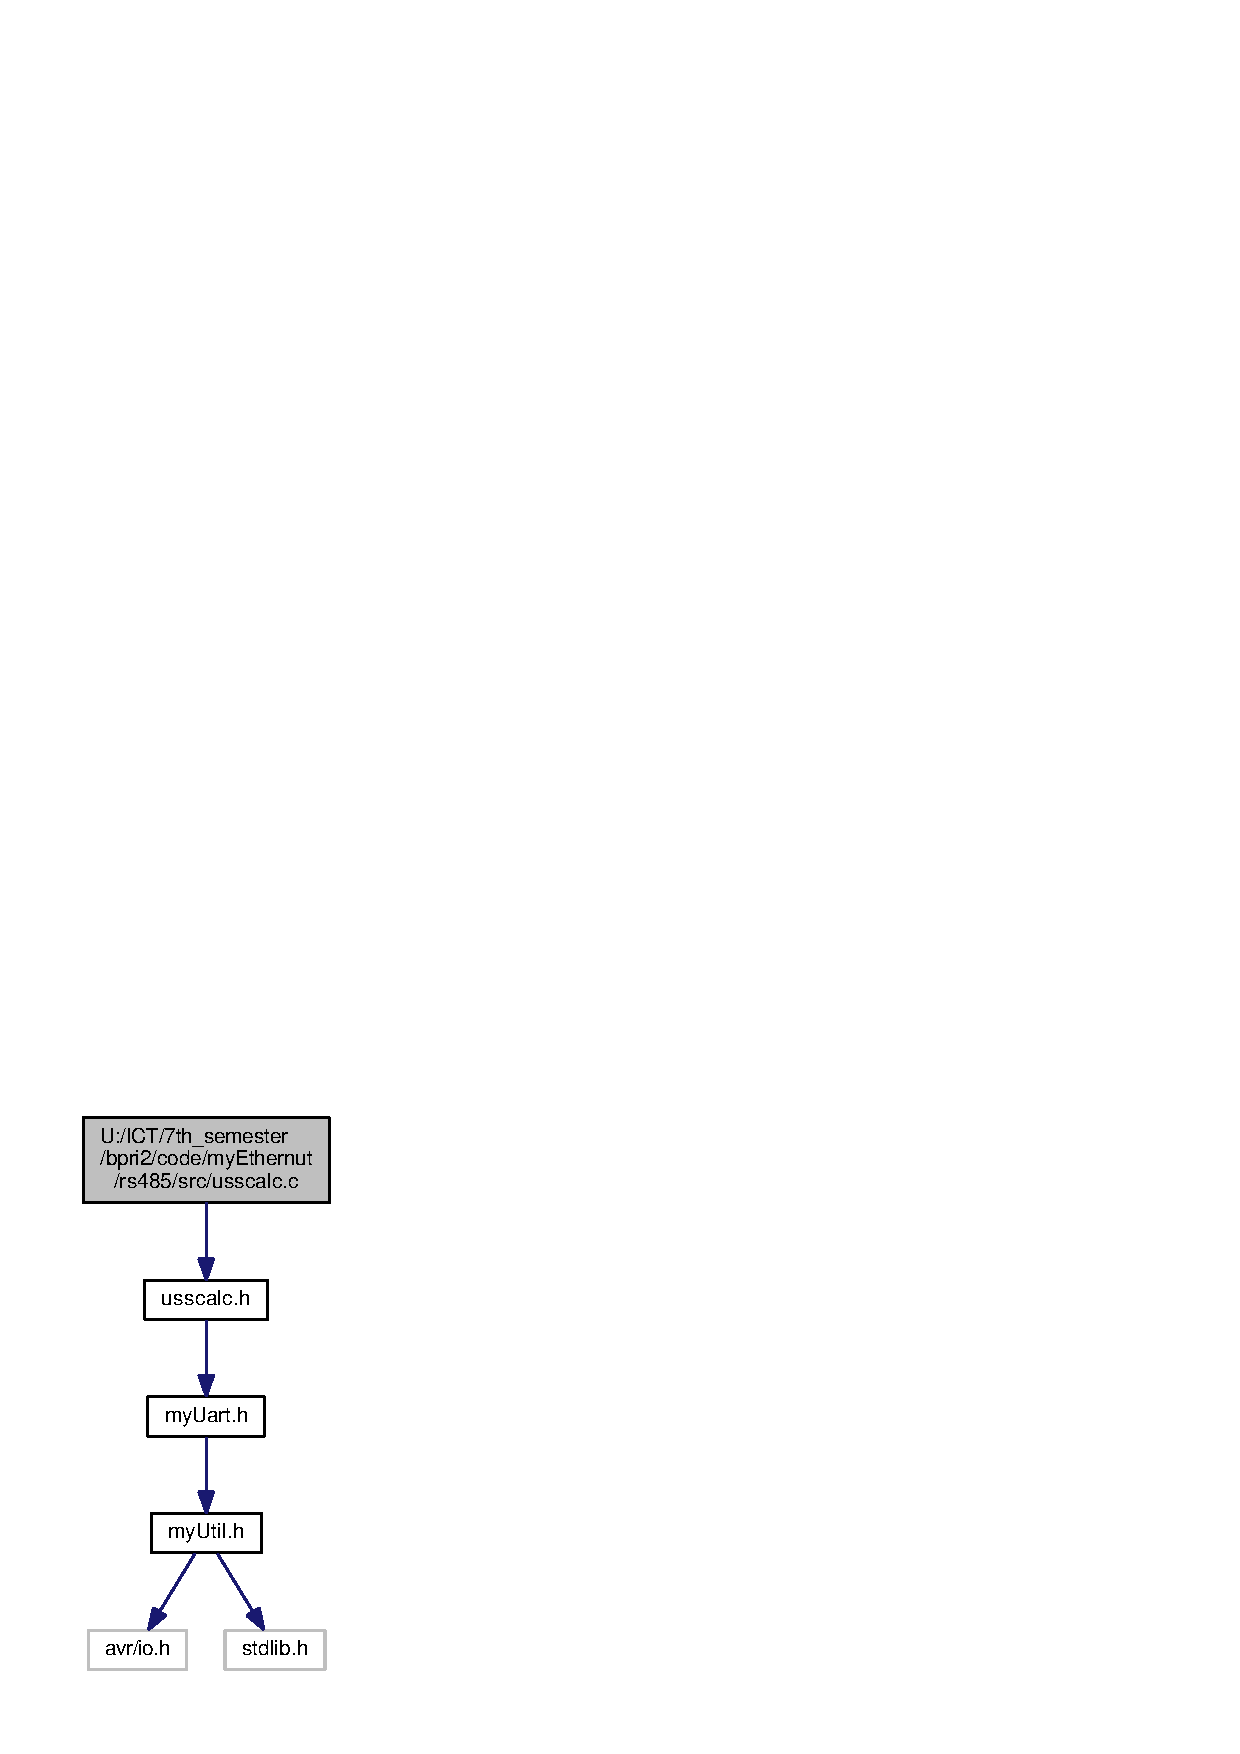
\includegraphics[width=162pt]{usscalc_8c__incl}
\end{center}
\end{figure}
\subsection*{Macros}
\begin{DoxyCompactItemize}
\item 
\#define {\bf ppo}~1
\item 
\#define {\bf mirror}~0
\item 
\#define {\bf pkw}~0
\item 
\#define {\bf A\+K}~0x00
\item 
\#define {\bf S\+P}~0
\item 
\#define {\bf P\+N\+U}~0x12bc
\item 
\#define {\bf P\+N\+Uex}~0x00
\item 
\#define {\bf I\+D\+X}~0x00
\end{DoxyCompactItemize}
\subsection*{Functions}
\begin{DoxyCompactItemize}
\item 
uint8\+\_\+t {\bf calc\+B\+C\+C} ()
\item 
void {\bf prep\+Telegram} (uint16\+\_\+t my\+Param)
\item 
uint16\+\_\+t {\bf get\+Value} (uint16\+\_\+t my\+Param)
\item 
void {\bf get\+All\+Values} (uint16\+\_\+t $\ast$mm\+Parameters\+Arr, uint8\+\_\+t length)
\end{DoxyCompactItemize}


\subsection{Macro Definition Documentation}
\index{usscalc.\+c@{usscalc.\+c}!A\+K@{A\+K}}
\index{A\+K@{A\+K}!usscalc.\+c@{usscalc.\+c}}
\subsubsection[{A\+K}]{\setlength{\rightskip}{0pt plus 5cm}\#define A\+K~0x00}\label{usscalc_8c_ac3a341ede33bbed651abe7f847361a6e}


Definition at line 29 of file usscalc.\+c.



Referenced by prep\+Telegram().

\index{usscalc.\+c@{usscalc.\+c}!I\+D\+X@{I\+D\+X}}
\index{I\+D\+X@{I\+D\+X}!usscalc.\+c@{usscalc.\+c}}
\subsubsection[{I\+D\+X}]{\setlength{\rightskip}{0pt plus 5cm}\#define I\+D\+X~0x00}\label{usscalc_8c_a223697fc2f8a4423171d86ced5c8872b}


Definition at line 41 of file usscalc.\+c.



Referenced by prep\+Telegram().

\index{usscalc.\+c@{usscalc.\+c}!mirror@{mirror}}
\index{mirror@{mirror}!usscalc.\+c@{usscalc.\+c}}
\subsubsection[{mirror}]{\setlength{\rightskip}{0pt plus 5cm}\#define mirror~0}\label{usscalc_8c_ab75be13d6d9ba70e2a9591121b408184}


Definition at line 20 of file usscalc.\+c.



Referenced by prep\+Telegram().

\index{usscalc.\+c@{usscalc.\+c}!pkw@{pkw}}
\index{pkw@{pkw}!usscalc.\+c@{usscalc.\+c}}
\subsubsection[{pkw}]{\setlength{\rightskip}{0pt plus 5cm}\#define pkw~0}\label{usscalc_8c_a0b9a09dbc3e3871baf2f518b82686dcb}


Definition at line 22 of file usscalc.\+c.

\index{usscalc.\+c@{usscalc.\+c}!P\+N\+U@{P\+N\+U}}
\index{P\+N\+U@{P\+N\+U}!usscalc.\+c@{usscalc.\+c}}
\subsubsection[{P\+N\+U}]{\setlength{\rightskip}{0pt plus 5cm}\#define P\+N\+U~0x12bc}\label{usscalc_8c_ab765f8aafdcbbd05cfcd27e208eb55b2}


Definition at line 35 of file usscalc.\+c.

\index{usscalc.\+c@{usscalc.\+c}!P\+N\+Uex@{P\+N\+Uex}}
\index{P\+N\+Uex@{P\+N\+Uex}!usscalc.\+c@{usscalc.\+c}}
\subsubsection[{P\+N\+Uex}]{\setlength{\rightskip}{0pt plus 5cm}\#define P\+N\+Uex~0x00}\label{usscalc_8c_a544eab7def9683a65c07c12fb091acc7}


Definition at line 38 of file usscalc.\+c.

\index{usscalc.\+c@{usscalc.\+c}!ppo@{ppo}}
\index{ppo@{ppo}!usscalc.\+c@{usscalc.\+c}}
\subsubsection[{ppo}]{\setlength{\rightskip}{0pt plus 5cm}\#define ppo~1}\label{usscalc_8c_a8ef3f4ce9afc84a8f4b4c62237ad2dcb}


Definition at line 18 of file usscalc.\+c.

\index{usscalc.\+c@{usscalc.\+c}!S\+P@{S\+P}}
\index{S\+P@{S\+P}!usscalc.\+c@{usscalc.\+c}}
\subsubsection[{S\+P}]{\setlength{\rightskip}{0pt plus 5cm}\#define S\+P~0}\label{usscalc_8c_aecd69d9a67487cc45c38eb184c50538a}


Definition at line 32 of file usscalc.\+c.



Referenced by prep\+Telegram().



\subsection{Function Documentation}
\index{usscalc.\+c@{usscalc.\+c}!calc\+B\+C\+C@{calc\+B\+C\+C}}
\index{calc\+B\+C\+C@{calc\+B\+C\+C}!usscalc.\+c@{usscalc.\+c}}
\subsubsection[{calc\+B\+C\+C()}]{\setlength{\rightskip}{0pt plus 5cm}uint8\+\_\+t calc\+B\+C\+C (
\begin{DoxyParamCaption}
{}
\end{DoxyParamCaption}
)}\label{usscalc_8c_a3758bfbaa4494e65cabf188a026502de}


Definition at line 43 of file usscalc.\+c.



References my\+Telegram.



Referenced by prep\+Telegram().

\index{usscalc.\+c@{usscalc.\+c}!get\+All\+Values@{get\+All\+Values}}
\index{get\+All\+Values@{get\+All\+Values}!usscalc.\+c@{usscalc.\+c}}
\subsubsection[{get\+All\+Values(uint16\+\_\+t $\ast$mm\+Parameters\+Arr, uint8\+\_\+t length)}]{\setlength{\rightskip}{0pt plus 5cm}void get\+All\+Values (
\begin{DoxyParamCaption}
\item[{uint16\+\_\+t $\ast$}]{mm\+Parameters\+Arr, }
\item[{uint8\+\_\+t}]{length}
\end{DoxyParamCaption}
)}\label{usscalc_8c_a0e6157d1764f0cd0bfd6895d2888d0f1}


Definition at line 106 of file usscalc.\+c.



References get\+Value().



Referenced by main().



Here is the call graph for this function\+:\nopagebreak
\begin{figure}[H]
\begin{center}
\leavevmode
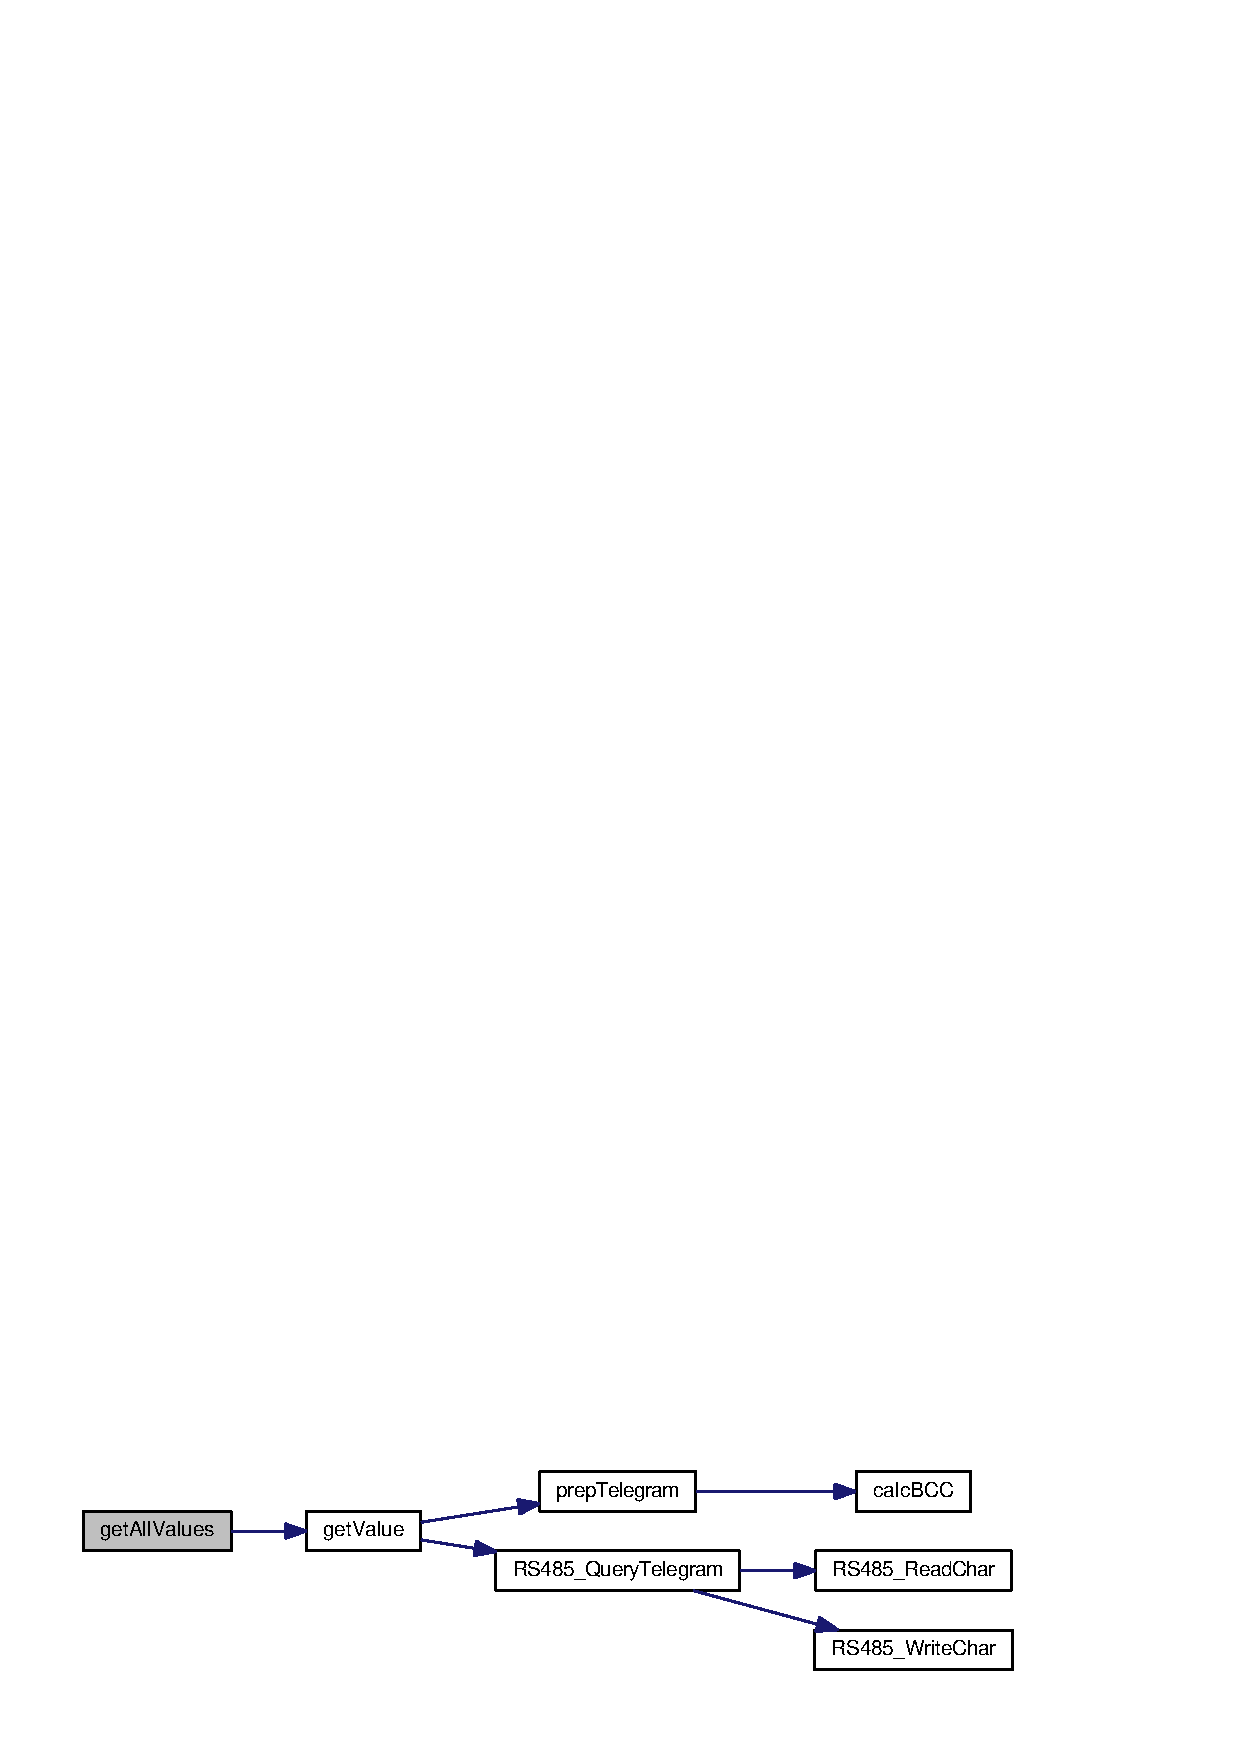
\includegraphics[width=350pt]{usscalc_8c_a0e6157d1764f0cd0bfd6895d2888d0f1_cgraph}
\end{center}
\end{figure}


\index{usscalc.\+c@{usscalc.\+c}!get\+Value@{get\+Value}}
\index{get\+Value@{get\+Value}!usscalc.\+c@{usscalc.\+c}}
\subsubsection[{get\+Value(uint16\+\_\+t my\+Param)}]{\setlength{\rightskip}{0pt plus 5cm}uint16\+\_\+t get\+Value (
\begin{DoxyParamCaption}
\item[{uint16\+\_\+t}]{my\+Param}
\end{DoxyParamCaption}
)}\label{usscalc_8c_a0d092db893cddedce1266d2971f2cd7f}


Definition at line 100 of file usscalc.\+c.



References my\+Telegram, prep\+Telegram(), and R\+S485\+\_\+\+Query\+Telegram().



Referenced by get\+All\+Values().



Here is the call graph for this function\+:\nopagebreak
\begin{figure}[H]
\begin{center}
\leavevmode
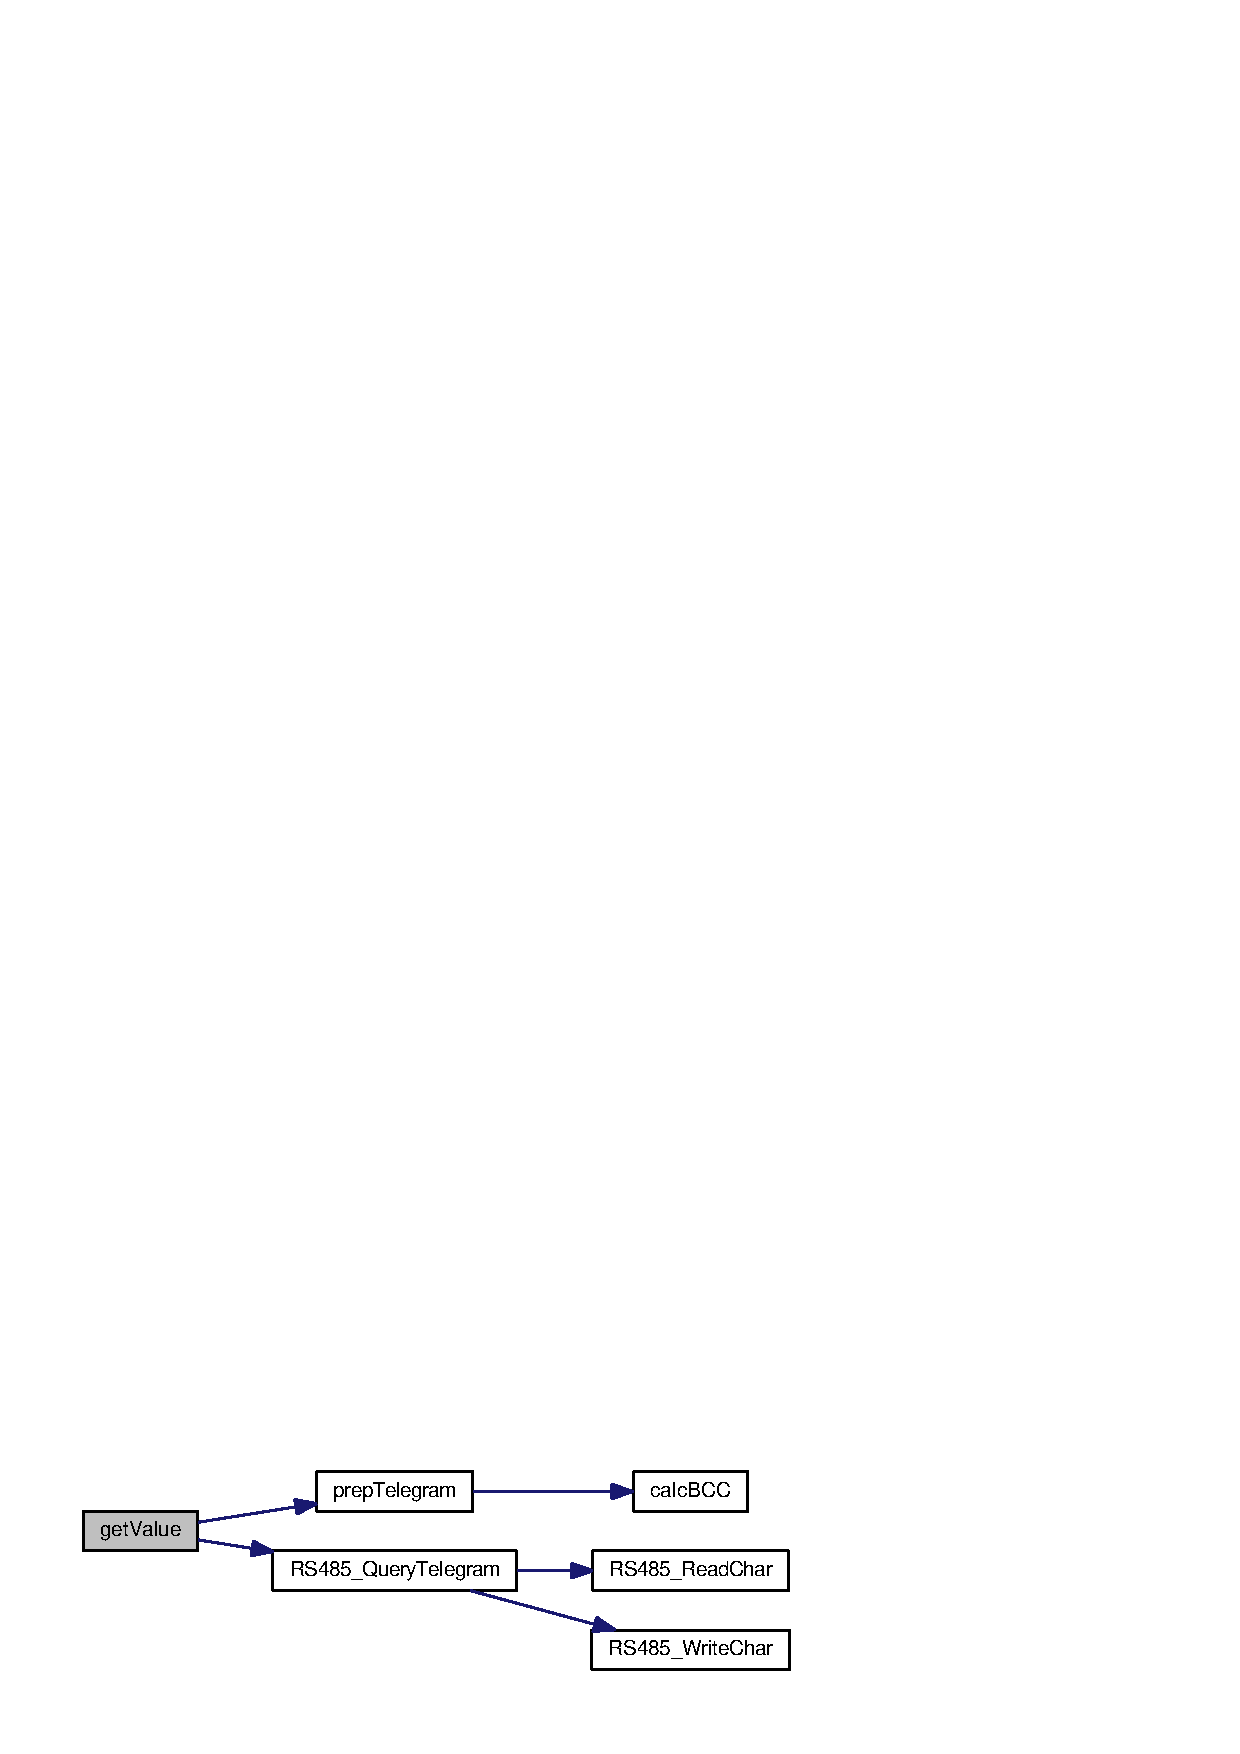
\includegraphics[width=350pt]{usscalc_8c_a0d092db893cddedce1266d2971f2cd7f_cgraph}
\end{center}
\end{figure}


\index{usscalc.\+c@{usscalc.\+c}!prep\+Telegram@{prep\+Telegram}}
\index{prep\+Telegram@{prep\+Telegram}!usscalc.\+c@{usscalc.\+c}}
\subsubsection[{prep\+Telegram(uint16\+\_\+t my\+Param)}]{\setlength{\rightskip}{0pt plus 5cm}void prep\+Telegram (
\begin{DoxyParamCaption}
\item[{uint16\+\_\+t}]{my\+Param}
\end{DoxyParamCaption}
)}\label{usscalc_8c_ac734b72553a80042ac173bfebf6b5185}


Definition at line 55 of file usscalc.\+c.



References A\+K, calc\+B\+C\+C(), I\+D\+X, mirror, my\+Telegram, and S\+P.



Referenced by get\+Value().



Here is the call graph for this function\+:\nopagebreak
\begin{figure}[H]
\begin{center}
\leavevmode
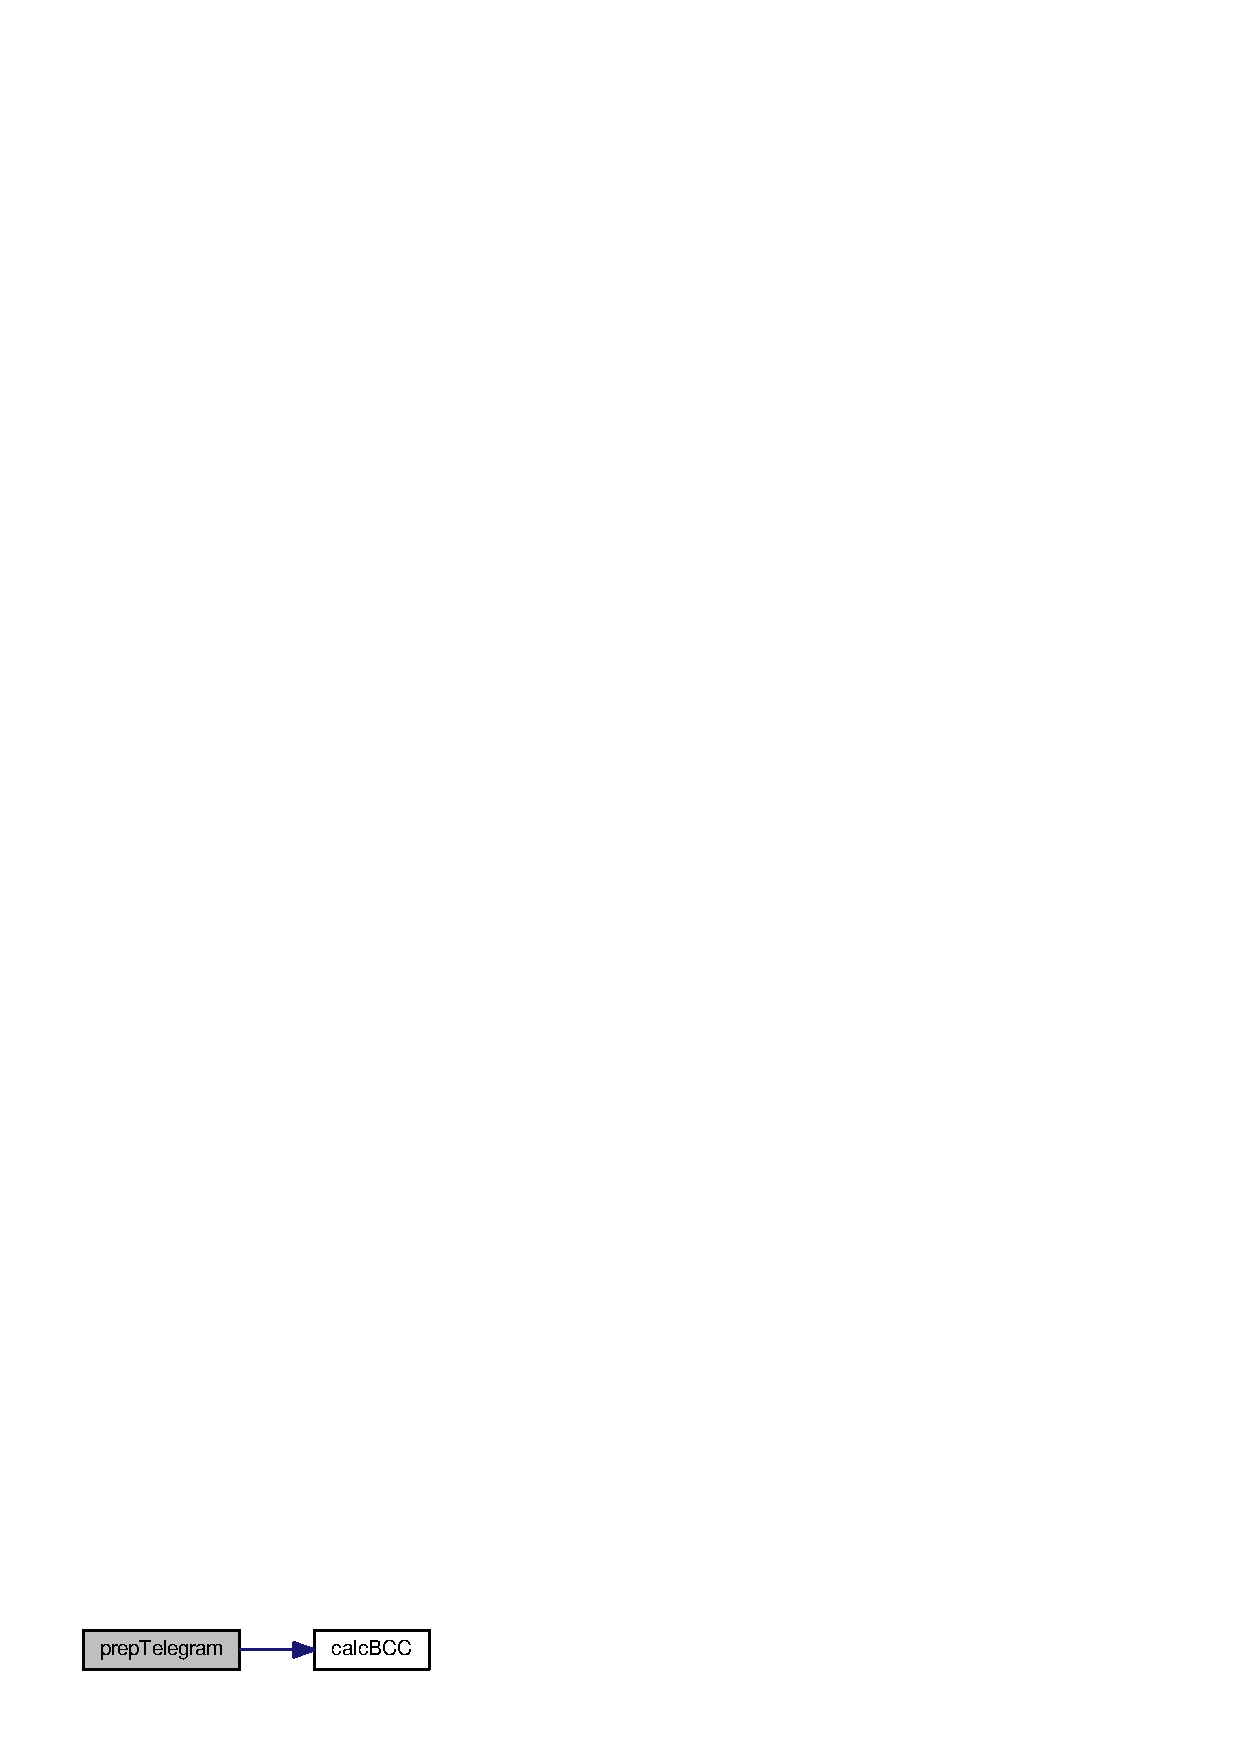
\includegraphics[width=210pt]{usscalc_8c_ac734b72553a80042ac173bfebf6b5185_cgraph}
\end{center}
\end{figure}



\section{U\+:/\+I\+C\+T/7th\+\_\+semester/bpri2/code/my\+Ethernut/rs485/src/usscalc.h File Reference}
\label{usscalc_8h}\index{U\+:/\+I\+C\+T/7th\+\_\+semester/bpri2/code/my\+Ethernut/rs485/src/usscalc.\+h@{U\+:/\+I\+C\+T/7th\+\_\+semester/bpri2/code/my\+Ethernut/rs485/src/usscalc.\+h}}
{\ttfamily \#include \char`\"{}my\+Uart.\+h\char`\"{}}\\*
Include dependency graph for usscalc.\+h\+:\nopagebreak
\begin{figure}[H]
\begin{center}
\leavevmode
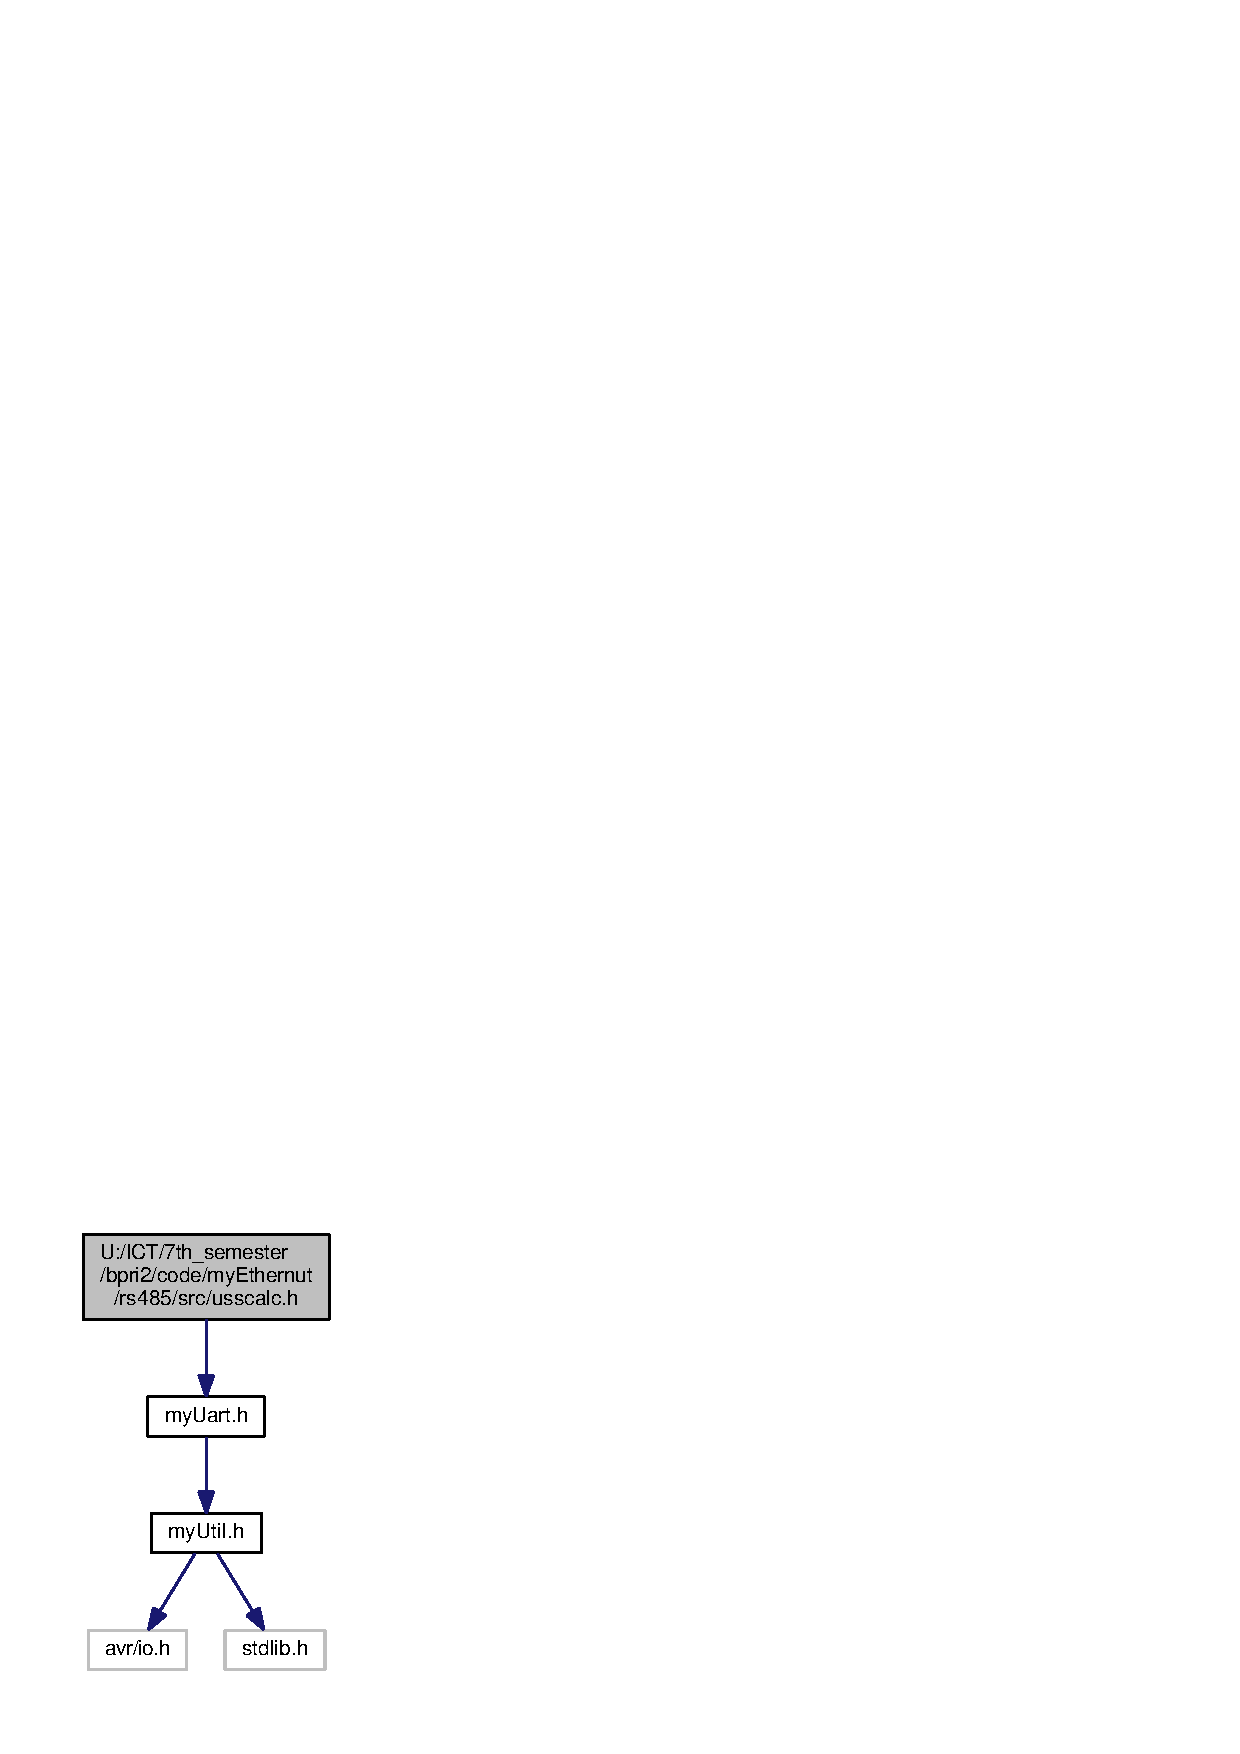
\includegraphics[width=162pt]{usscalc_8h__incl}
\end{center}
\end{figure}
This graph shows which files directly or indirectly include this file\+:\nopagebreak
\begin{figure}[H]
\begin{center}
\leavevmode
\includegraphics[width=298pt]{usscalc_8h__dep__incl}
\end{center}
\end{figure}
\subsection*{Functions}
\begin{DoxyCompactItemize}
\item 
uint16\+\_\+t {\bf get\+Value} (uint16\+\_\+t my\+Param)
\item 
void {\bf get\+All\+Values} (uint16\+\_\+t $\ast$my\+Param\+Arr, uint8\+\_\+t length)
\end{DoxyCompactItemize}
\subsection*{Variables}
\begin{DoxyCompactItemize}
\item 
uint8\+\_\+t {\bf my\+Telegram} [14]
\end{DoxyCompactItemize}


\subsection{Function Documentation}
\index{usscalc.\+h@{usscalc.\+h}!get\+All\+Values@{get\+All\+Values}}
\index{get\+All\+Values@{get\+All\+Values}!usscalc.\+h@{usscalc.\+h}}
\subsubsection[{get\+All\+Values(uint16\+\_\+t $\ast$my\+Param\+Arr, uint8\+\_\+t length)}]{\setlength{\rightskip}{0pt plus 5cm}void get\+All\+Values (
\begin{DoxyParamCaption}
\item[{uint16\+\_\+t $\ast$}]{my\+Param\+Arr, }
\item[{uint8\+\_\+t}]{length}
\end{DoxyParamCaption}
)}\label{usscalc_8h_ad7a9eba4da373dcceca0624ff97121d4}


Definition at line 106 of file usscalc.\+c.



References get\+Value().



Referenced by main().



Here is the call graph for this function\+:\nopagebreak
\begin{figure}[H]
\begin{center}
\leavevmode
\includegraphics[width=350pt]{usscalc_8h_ad7a9eba4da373dcceca0624ff97121d4_cgraph}
\end{center}
\end{figure}


\index{usscalc.\+h@{usscalc.\+h}!get\+Value@{get\+Value}}
\index{get\+Value@{get\+Value}!usscalc.\+h@{usscalc.\+h}}
\subsubsection[{get\+Value(uint16\+\_\+t my\+Param)}]{\setlength{\rightskip}{0pt plus 5cm}uint16\+\_\+t get\+Value (
\begin{DoxyParamCaption}
\item[{uint16\+\_\+t}]{my\+Param}
\end{DoxyParamCaption}
)}\label{usscalc_8h_a0d092db893cddedce1266d2971f2cd7f}


Definition at line 100 of file usscalc.\+c.



References my\+Telegram, prep\+Telegram(), and R\+S485\+\_\+\+Query\+Telegram().



Referenced by get\+All\+Values().



Here is the call graph for this function\+:\nopagebreak
\begin{figure}[H]
\begin{center}
\leavevmode
\includegraphics[width=350pt]{usscalc_8h_a0d092db893cddedce1266d2971f2cd7f_cgraph}
\end{center}
\end{figure}




\subsection{Variable Documentation}
\index{usscalc.\+h@{usscalc.\+h}!my\+Telegram@{my\+Telegram}}
\index{my\+Telegram@{my\+Telegram}!usscalc.\+h@{usscalc.\+h}}
\subsubsection[{my\+Telegram}]{\setlength{\rightskip}{0pt plus 5cm}uint8\+\_\+t my\+Telegram[14]}\label{usscalc_8h_ace4b9a76218fd1cc485563419811a46b}


Definition at line 6 of file usscalc.\+h.



Referenced by calc\+B\+C\+C(), get\+Value(), prep\+Telegram(), and R\+S485\+\_\+\+Query\+Telegram().


%--- End generated contents ---

% Index
\backmatter
\newpage
\phantomsection
\clearemptydoublepage
\addcontentsline{toc}{chapter}{Index}
\printindex

\end{document}
